\documentclass[a4paper,nobib]{tufte-book}

\hypersetup{colorlinks}% uncomment this line if you prefer colored hyperlinks (e.g., for onscreen viewing)

%%
% If they're installed, use Bergamo and Chantilly from www.fontsite.com.
% They're clones of Bembo and Gill Sans, respectively.
%\IfFileExists{bergamo.sty}{\usepackage[osf]{bergamo}}{}% Bembo
%\IfFileExists{chantill.sty}{\usepackage{chantill}}{}% Gill Sans

%\usepackage[protrusion=true,expansion,babel=true]{microtype}

%%
% Just some sample text
\usepackage{lipsum}

%%
% For nicely typeset tabular material
\usepackage{booktabs}
\usepackage{multirow}
\usepackage{adjustbox}
\usepackage{array}

\newcolumntype{L}[1]{>{\noindent\RaggedRight\arraybackslash\hspace{0pt}}p{#1}}
\newcolumntype{R}[1]{>{\noindent\RaggedLeft\arraybackslash\hspace{0pt}}p{#1}}
\newcolumntype{C}[1]{>{\noindent\Centering\arraybackslash\hspace{0pt}}p{#1}}

%%
% For graphics / images
\usepackage{graphicx}
\setkeys{Gin}{width=\linewidth,totalheight=\textheight,keepaspectratio}
\graphicspath{{media/}}

% What
\setcounter{secnumdepth}{3}
\setcounter{tocdepth}{3}

% Bibliography
\usepackage[
style=ieee,
citestyle=numeric-comp,
autocite=inline,
autopunct=true,
backend=biber,
maxbibnames=99,
maxcitenames=2,
mincitenames=1,
]{biblatex}
\addbibresource{bibliography.bib}


%%
% Maths
\usepackage{amsmath}

% Prints a trailing space in a smart way.
\usepackage{xspace}

% Inserts a blank page
\newcommand{\blankpage}{\newpage\hbox{}\thispagestyle{empty}\newpage}

% Referencing
\usepackage[unicode]{hyperref}
\usepackage[nameinlink]{cleveref}

\hypersetup{%
	bookmarksnumbered = true, % Show section numbering in the PDF table of contents. Allows easier browsing of the document
	colorlinks = true, % uncomment this line if you prefer colored hyperlinks (e.g., for onscreen viewing)
%	pdfborder = {0 0 0},
	bookmarksdepth = subsection,
%	citecolor = DarkGreen,
%	linkcolor = DarkBlue,
%	urlcolor = DarkGreen,
}

%\AtBeginDocument{%
%	\hypersetup{
%		pdfauthor={\plainauthor}
%		pdftitle={\plaintitle},
%	}%
%}

\usepackage[binary-units=true]{siunitx}

% Modifications to the default tufte template to make it more applicable to a thesis
% Credit goes to Tiffany Tseng, lalider, see https://github.com/lalider/tufte-latex-thesis

\usepackage[parfill]{parskip}

% remove paragraph indentation
\makeatletter
% Paragraph indentation and separation for normal text
\renewcommand{\@tufte@reset@par}{%
	\setlength{\RaggedRightParindent}{0.0pc}%
	\setlength{\JustifyingParindent}{0.0pc}%
	\setlength{\parindent}{0pc}%
	\setlength{\parskip}{\baselineskip}%
}
\@tufte@reset@par

% Paragraph indentation and separation for marginal text
\renewcommand{\@tufte@margin@par}{%
	\setlength{\RaggedRightParindent}{0.0pc}%
	\setlength{\JustifyingParindent}{0.0pc}%
	\setlength{\parindent}{0.0pc}%
	\setlength{\parskip}{10pt}%
}
\makeatother

\titleformat{\section}%
[hang]% shape
{\normalfont\Large}% format applied to label+text
{\thesection}% label
{1em}% horizontal separation between label and title body
{}% before the title body
[]% after the title body

%\titlespacing*{\section}{0pt}{3.5ex plus 1ex minus .2ex}{2.3ex plus .2ex}
%\titlespacing*{\subsection}{0pt}{3.25ex plus 1ex minus .2ex}{1.5ex plus.2ex}
\titlespacing*{\section}{0pt}{30pt}{20pt}
\titlespacing*{\subsection}{0pt}{20pt}{5pt}


% Disable adding empty pages without a purpose (not intended for printing in a book format...)
\makeatletter
\def\cleardoublepage{
	\clearpage%
}
\makeatother

% Acronyms
\usepackage{acro}
\acsetup{
	use-id-as-short,
	make-links=false,
	case-sensitive=false,
	patch/floats=false,
	patch/caption=false,
	patch/tabularx=false
}
\DeclareAcronym{FDIR}{short=FDIR,long={Fault Detection, Isolation and Recovery}}
\DeclareAcronym{ADCS}{short = ADCS, long = {Attitude Determination and Control Subsystem}}
\DeclareAcronym{COMMS}{short = COMMS, long = {Communications}}
\DeclareAcronym{EPS}{short = EPS, long = {Electrical Power Subsystem}}
\DeclareAcronym{OBC}{short = OBC, long = {On-Board Computer}}
\DeclareAcronym{OBDH}{short = OBDH, long = {On-Board Data Handling}}
\DeclareAcronym{OBSW}{short = OBSW, long = {On-Board Software}}
\DeclareAcronym{OPS}{short = OPS, long = {Operations}}
\DeclareAcronym{SYE}{short = SYE, long = {Systems Engineering}}
\DeclareAcronym{SU}{short = SU, long = {Science Unit}}
\DeclareAcronym{EMC}{short = EMC, long = {Electromagnetic Compatibility}}
\DeclareAcronym{CDR}{short = CDR, long = {Critical Design Review}}
\DeclareAcronym{GS}{short = GS, long = {Ground Station}}
\DeclareAcronym{TC}{short = TC, long = Telecommands}
\DeclareAcronym{TM}{short = TM, long = Telemetry}
\DeclareAcronym{RF}{short = RF, long = RadioFrequency}
\DeclareAcronym{CCSDS}{short = CCSDS, long = {The Consultative Committee for Space Data Systems}}
\DeclareAcronym{ISM}{short = ISM, long = {Industrial, Scientific, Medical}}
\DeclareAcronym{COTS}{short = COTS, long = {Commercial Off-The-Shelf}}
\DeclareAcronym{PCDU}{short = PCDU, long = {Power Conditioning \& Distribution Unit}}
\DeclareAcronym{MPPT}{short = MPPT, long = {Maximum Power Point Tracking}}
\DeclareAcronym{ECSS}{short = ECSS, long = {European Cooperation for Space Standardization}}
\DeclareAcronym{PUS}{short = PUS, long = {Packet Utilisation Standard}}
\DeclareAcronym{UHF}{short = UHF, long = {Ultra-High Frequency}}
\DeclareAcronym{LEO}{short = LEO, long = {Low Earth Orbit}}
\DeclareAcronym{PDMS}{short = PDMS, long = {Polydimethylsiloxane}}
\DeclareAcronym{PA}{short = PA, long = {Product Assurance}}
\DeclareAcronym{PCB}{short = PCB, long = {Printed Circuit Board}}
\DeclareAcronym{GMAT}{short = GMAT, long = {General Mission Analysis Tool}}
\DeclareAcronym{MRAM}{short = MRAM, long = {Magnetoresistive Random-Access Memory}}
\DeclareAcronym{CAN}{short = CAN, long = {Controller Area Network}}
\DeclareAcronym{MCU}{short = MCU, long = {microcontroller}, extra={MicroController Unit}}
\DeclareAcronym{RTOS}{short = RTOS, long = {Real-Time Operating System}}
\DeclareAcronym{SAVOIR}{short = SAVOIR, long = {Space AVionics Open Interface aRchitecture}}
\DeclareAcronym{YAMCS}{short = YAMCS, long = {Yet Another Mission Control System}}
\DeclareAcronym{COBS}{short = COBS, long = {Consistent Overhead Byte Stuffing}}
\DeclareAcronym{SRAM}{short = SRAM, long = {Static Random Access Memory}}
\DeclareAcronym{I2C}{short = {I\textsuperscript{2}C}, long = {Inter-Integrated Circuit}}
\DeclareAcronym{ETL}{short = ETL, long = {Embedded Template Library}}
\DeclareAcronym{HAL}{short = HAL, long = {Hardware Abstraction Library}}
\DeclareAcronym{IDE}{short = IDE, long = {Integrated Development Environment}}
\DeclareAcronym{USB}{short = USB, long = {Universal Serial Bus}}
\DeclareAcronym{UART}{short = UART, long = {Universal Asynchronous Serial Bus}}
\DeclareAcronym{FMEA}{short = FMEA, long = {Failure Mode and Effects Analysis}}
\DeclareAcronym{FMECA}{short = FMECA, long = {Failure Mode, Effects and Criticality Analysis}}
\DeclareAcronym{HSIA}{short = HSIA, long = {Hardware/Software Interaction Analysis}}
\DeclareAcronym{XTCE}{short = XTCE, long = {XML Telemetric and Command Exchange}}
\DeclareAcronym{RAMS}{short = RAMS, long = {Reliability, Availability, Maintainability and Safety}}
\DeclareAcronym{MAIV}{short = MAIV, long = {Maintenance, Assembly, Integration and Verification}}
\DeclareAcronym{IC}{short = IC, long = {Integrated Circuit}}
\NewDocumentCommand\draft{m}{%
	\textcolor[HTML]{bf616a}{#1}%
}

\makeatletter
\newcommand\footurl@[1]{\footnote{\url@{#1}}}
\DeclareRobustCommand{\footurl}{\hyper@normalise\footurl@}

\newcommand\foothref@[2]{\href@{#1}{#2}\footnote{\url@{#1}}}
\def\Hy@foothref#{%
	\hyper@normalise\foothref@
}
\DeclareRobustCommand*{\foothref}[1][]{%
	\begingroup
	\setkeys{href}{#1}%
	\@ifnextchar\bgroup\Hy@foothref{\hyper@normalise\foothref@}%
}
\makeatother

% Transitions
\AtBeginDocument{
\colorlet{invalid}{MaterialAmber900}
\colorlet{unexpected}{MaterialRed900}
}

\def\unchecked{\textcolor{MaterialGrey800}{\texttt{Unchecked}}}
\def\ok{\texttt{OK}}
\def\unexpected{\textcolor{unexpected}{\texttt{Unexpected\_Value}}}
\def\hilim{\textcolor{unexpected}{\texttt{Above\_High\_Limit}}}
\def\lolim{\textcolor{unexpected}{\texttt{Below\_Low\_Limit}}}
\def\invalid{\textcolor{invalid}{\texttt{Invalid}}}
\def\ar{ \( \rightarrow \) }

\makeatletter

\makeatother

\NewAcroTemplate[list]{glossary}{%
	\begin{description}
		\acronymsmapF{%
			\item[\sffamily\textbf{\acrowrite{short}}] \acrowrite{long}%
			\acroifanyT {foreign,extra} {~(}%
			\acrowrite {foreign}%
			\acroifallT {foreign,extra} {,~}%
			\acrowrite {extra}%
			\acroifanyT {foreign,extra} {)}%
			\acropagefill%
			\acropages%
				{ \acrotranslate {page} \nobreakspace }%
				{ \acrotranslate {pages} \nobreakspace }%
		}%
		{ \item \AcroRerun{list} }%
		\end {description}
	}

% Various utilities
\usepackage{tabularx}
\usepackage[singlelinecheck=false]{caption}
\usepackage{subcaption}
\usepackage{comment}

% Generates the index
\usepackage{makeidx}
\makeindex

\usepackage{tikz}
\usepackage{pgfplots}
\pgfplotsset{compat = 1.3}
\usetikzlibrary{pie}
\usepackage{physics}
\let\Re=\relax
\let\Im=\relax

% Colours
\definecolor{off}{HTML}{e53935}
\definecolor{on}{HTML}{43a047}
\usepackage{xcolor-solarized}
\usepackage{xcolor-material}
\usepackage{colortbl}

%\usepackage{todonotes}
\usepackage{enumitem}
\usepackage[absolute,overlay]{textpos}

% Code
\usepackage{minted}
\usepackage{xpatch,letltxmacro}
\LetLtxMacro{\cminted}{\minted}
\let\endcminted\endminted
\xpretocmd{\cminted}{\RecustomVerbatimEnvironment{Verbatim}{BVerbatim}{}}{}{}
\definecolor{mintedbg}{rgb}{0.95,0.95,0.93}
\setminted{
	bgcolor=mintedbg,
	tabsize=2
}
\setminted[text]{baselinestretch=0.8}

% Git magic
\makeatletter
\write18{git log --pretty='format:\@percentchar Creset\@percentchar s' --no-merges -1 > \jobname.git1.tmp}
\write18{git rev-parse --short HEAD > \jobname.git2.tmp}
\def\gitcommit{\input{\jobname.git2.tmp}\unskip}
\def\gitcommitmessage{\input{\jobname.git1.tmp}\unskip}
\makeatother

% Smart citations

\makeatletter

%\def\blx@imc@mkbibquote{\blx@enquote}

\newbibmacro*{cite:title}{%
  \printtext[bibhyperref]{%
    \printfield[citetitle]{labeltitle}}%
  \finentry}

\newbibmacro*{cite:shorthand}{%
	\printtext[bibhyperref]{\printfield{shorthand}}}

\newbibmacro*{cite:full}{%
	\iffieldundef{shorthand}
	{\printnames{labelname}%
		\setunit*{\printdelim{nametitledelim}}%
		\usebibmacro{cite:title}}%
	{\usebibmacro{cite:shorthand}}}

\newbibmacro*{cite:marginnote}{%
	\marginnote{%
		% \mkbibbrackets should be used here probably
		[%
			\printfield{labelprefix}%
			\printfield{labelnumber}%
		]
		\usebibmacro{cite:full}%
	}%
}

\DeclareCiteCommand{\dualcite}[\mkbibbrackets]
  {\usebibmacro{cite:init}%
   \usebibmacro{prenote}}
  {\usebibmacro{citeindex}%
   \usebibmacro{cite:marginnote}%
   \usebibmacro{cite:comp}}%
  {}
  {\usebibmacro{cite:dump}%
   \usebibmacro{postnote}}

\def\tuftecite{
	\iffootnote{footnote}{text}
}

% Patching commands that enter information in margins, so that we can detect which
% citation should be used
\newtoggle{inmargin}
\pretocmd{\marginpar}{\toggletrue{inmargin}}{}{}
\apptocmd{\@xympar}{\togglefalse{inmargin}}{}{}
\pretocmd{\@tufte@float}{\toggletrue{inmargin}}{}{}
\pretocmd{\end@tufte@float}{\togglefalse{inmargin}}{}{}
\pretocmd{\@tufte@margin@float}{\toggletrue{inmargin}}{}{}
\pretocmd{\end@tufte@margin@float}{\togglefalse{inmargin}}{}{}

\def\autocite{%
	\iftoggle{inmargin}\parencite\dualcite%
}

% Tufte disables subparagraphs. This brings them back.
\renewcommand\subparagraph{\@startsection{subparagraph}{5}{\parindent}%
	{3.25ex \@plus1ex \@minus .2ex}%
	{-1em}%
	{\hspace{1em}\normalfont\normalsize\itshape}}

% \acuse command that also adds the current page
%\NewAcroTemplate{fdirthesisempty}{}
%\NewAcroCommand\acusepage{m}{}
\let\acusepage\acuse

\makeatother

%%
% Book metadata
\title{Design of Fault Detection, Isolation and Recovery in the AcubeSAT nanosatellite\thanks{AcubeSAT}}
\author[Konstantinos Kanavouras]{Konstantinos Kanavouras}
\publisher{Aristotle University of Thessaloniki}

\acsetup{foreign/display=false, list/foreign/display=false}

\def\g{\ignorespaces}
\def\e{\ignorespaces}
\def\acusepage#1{}

\usepackage{microtype}

\begin{document}

% Front matter
%\frontmatter

% r.1 blank page
%\blankpage

% r.3 full title page
\makeatletter
\renewcommand{\maketitle}{%
	\newpage
	\global\@topnum\z@% prevent floats from being placed at the top of the page
	\begingroup
	\setlength{\parindent}{0pt}%
	\setlength{\parskip}{4pt}%
	\let\@@title\@empty
	\let\@@author\@empty
	\let\@@date\@empty
	\thispagestyle{empty}
	\begin{fullwidth}
		\vfill
		\begin{center}
			\href{https://www.auth.gr/}{
\includegraphics[width=.8\textwidth]{auth_logo_text}}\par
			\vspace{1cm}
			\LARGE\textsc{Diploma Thesis}\par
			\vspace{6ex}
			\hrule
			\vspace{4ex}
			\Huge\textbf{Design of Fault Detection, Isolation and Recovery}\\[1ex]
			\LARGE\textbf{in the}\\
			\Huge\textbf{AcubeSAT NanoSatellite}\par
			\vspace{2.7ex}
			\hrule

			\vspace{6ex}

			\Large
			\begin{tabular}{ll}
				\emph{Author:} & \href{https://github.com/kongr45gpen}{Konstantinos \textsc{Kanavouras} \normalsize (\fontfamily{pplx}\selectfont 8824)}
				\\[1.5ex]
				\emph{Supervisor:} & \href{http://ee.auth.gr/en/school/faculty-staff/electronics-computers-department/hatzopoulos-alkiviadis/}{Prof. Alkiviadis \textsc{Hatzopoulos}}
			\end{tabular}

			\vspace{6ex}

			\large \textit{A thesis submitted in fulfillment of the requirements\\ for the diploma in Electrical \& Computer Engineering}\\[0.3cm] % University requirement text
			\textit{in the}\\[0.4cm]
			\href{https://www.eng.auth.gr/en/home.html}{Faculty of Engineering}
			\\
			\href{https://ee.auth.gr/en/}{Electrical \& Computer Engineering Department}
			\\[1cm] % Research group name and department name

			\vspace{6ex}

			{\large June 28, 2021}\\[4cm] % Date

		\end{center}
		\vfill
	\end{fullwidth}
	\endgroup
	\thispagestyle{plain}% suppress the running head
	\tuftebreak% add some space before the text begins
	\@afterindentfalse\@afterheading% suppress indentation of the next paragraph
}
\makeatother
\maketitle

% v.4 copyright page
\newpage
\begin{fullwidth}
~\vfill
\thispagestyle{empty}
\setlength{\parindent}{0pt}
\setlength{\parskip}{\baselineskip}
Copyright \copyright\ \the\year\ \thanklessauthor

\par\smallcaps{Published by the \thanklesspublisher}

\par\smallcaps{\href{https://github.com/kongr45gpen/thesis-latex}{Https://GitHub.com/Kongr45gpen/Thesis-Latex}}

\justify

\par Licensed under the Creative Commons Attribution 4.0 International (CC BY 4.0) License (the ``License''); you may not
use this file except in compliance with the License. You may obtain a copy
of the License at \url{https://creativecommons.org/licenses/by/4.0/legalcode}, or a human-readable summary at \url{https://creativecommons.org/licenses/by/4.0/}.
Unless
required by applicable law or agreed to in writing, material distributed
under the License is distributed on an \smallcaps{``AS IS'' BASIS, WITHOUT
WARRANTIES OR CONDITIONS OF ANY KIND}, either express or implied. See the
License for the specific language governing permissions and limitations
under the License.\index{license}

\par This thesis was produced using \LaTeX, the \href{https://ctan.org/pkg/tufte-latex?lang=en}{\texttt{tufte-latex}} template, and the modifications from \linebreak[4] \href{https://github.com/lalider/tufte-latex-thesis}{\texttt{tufte-latex-thesis}}.

\par This document is an unofficial translation of the \href{https://ikee.lib.auth.gr/record/332377/?ln=en}{thesis transcript submitted to the University}, completed by the author.

\par The AcubeSAT project is carried out with the support of the Education Office of the \href{https://www.esa.int/}{European Space Agency}, under the educational \href{https://www.esa.int/Education/CubeSats_-_Fly_Your_Satellite/}{Fly Your Satellite! programme}.

\par The views expressed herein by the authors can \smallcaps{in no way be taken to reflect} the official opinion, or endorsement, of the European Space Agency.

\par\textit{Rendered on \today{} (\texttt{\gitcommit}: \gitcommitmessage)}
\end{fullwidth}

% r.5 contents
\tableofcontents

\begin{fullwidth}
\listoffigures

\listoftables

%\chapter*{List of Acronyms}
%\acuseall%
\bgroup
\setlength\parskip{1ex}
\printacronyms[pages={display=all,seq/use=false},]
\egroup

\end{fullwidth}

% r.9 introduction
\cleardoublepage

\chapter*{Abstract}

\justify
Space is not a welcoming environment; while the aerospace engineering community has managed to reliably operate thousands of satellites in orbit, CubeSats, the most popular class of nanosatellite, only have a 50\% success rate. Low costs, lack of strict technical requirements and scarcity of publicly available documentation often drive up the risks for educational, scientific and commercial CubeSats. This thesis investigates a configurable and modular Fault Detection, Isolation and Recovery (FDIR) architecture that uses the ECSS Packet Utilisation Standard. This FDIR concept, along with the provided open-source software implementation, can be used by CubeSat missions to increase the reliability of their design and chances of mission success, by autonomously responding to on-board errors. The thesis also includes background information regarding CubeSat reliability, and explores the software and hardware used to implement the proposed FDIR design on the AcubeSAT mission, currently under design by students of the Aristotle University of Thessaloniki.

%%
% Start the main matter (normal chapters)
\mainmatter


\chapter{Introduction}

\section{Thesis research area}


\begin{marginfigure}
	\centering
	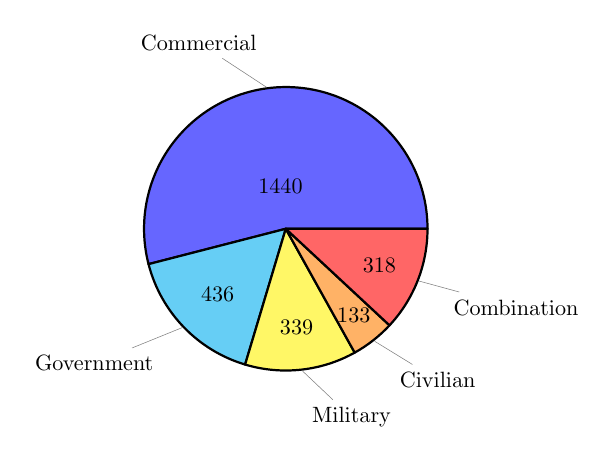
\begin{tikzpicture}[every node/.style={scale=.8}]
	\pie[
	sum=auto,after number=,radius={1.8},text=pin
	]{1440/Commercial,
		436/Government,
		339/Military,
		133/Civilian,
		318/Combination
	}
	
	\end{tikzpicture}
	\caption[Types of satellites in operation in 2018]{Types of satellites in operation in 2018 \autocite{wood_visualizing_all_2020}}
	\label{fig:satellite_types}
\end{marginfigure}

This thesis involves satellite design and operations, parts of the Aerospace Engineering disciplines. The first artificial satellite \e{``Sputnik 1''} was launched in 1957, and by 2021 about 8900 satellites have been launched, of which about 4000 are currently operational and in orbit \autocite{unionofconcernedscientists_satellite_database_2021,kelso_norad_twoline,wood_visualizing_all_2020}.

Artificial satellites can perform a number of different functions, which typically include telecommunications, earth observation, navigation (\acs{GNSS}), scientific research, technology demonstration, and other purposes, excluding manned missions, missions beyond Earth orbit, and space stations. The data generated using space technology have long been an integral part of modern civilisation, having influenced transportation, weather forecasting, and technology in general.

\begin{figure}
	\centering
	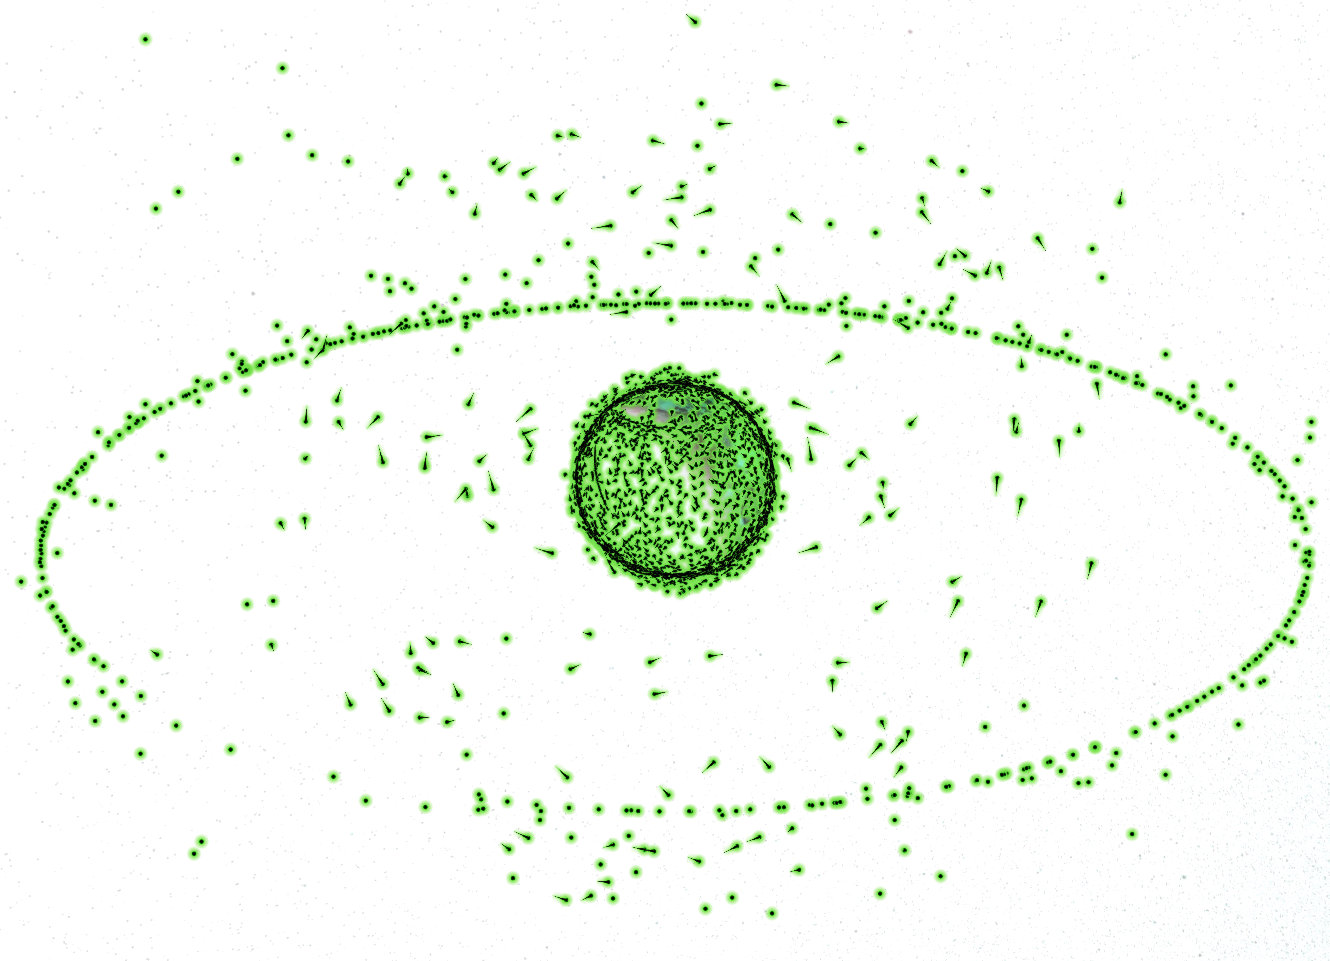
\includegraphics[width=.9\textwidth]{satellites}
	\caption[Active satellites orbiting the earth in 2021]{Active satellites orbiting the earth in 2021. \acl{LEO} satellites can be seen close to the planet, and Geostationary Orbit satellites can be seen at a fixed high altitude, while Medium Earth Orbit are between the two previous categories.}
				\label{fig:all_satellites}
				\setfloatalignment{t}
			\end{figure}
			
After launch, satellites typically remain in space until the completion of their mission after some years, at which point they can either return to Earth and burn up in the atmosphere, or remain in space as ``space junk''.

\begin{marginfigure}
	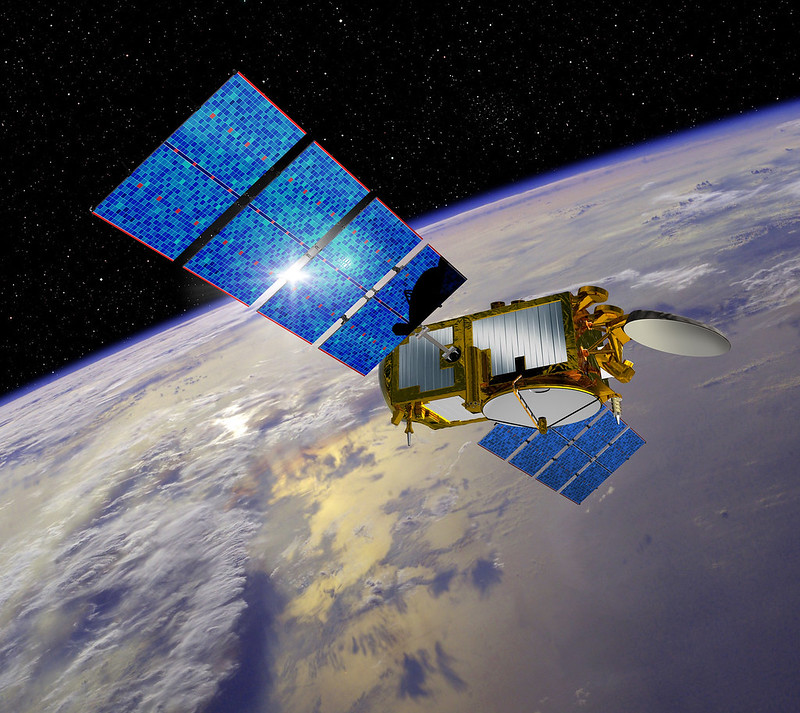
\includegraphics{cool_satellite}
	\caption[Artistic view of the Jason-3 satellite]{Artistic view of the \href{https://www.flickr.com/photos/noaasatellites/16979948568}{Jason-3} satellite} %The image shows the solar panels, the two directional antennas and the thermal insulation of the satellite.
\end{marginfigure}

Space technology developments present a significant degree of difficulty, which stems from the highly increased reliability requirements in the harsh environment of space. In particular, the long distances, extreme temperatures, mechanical launch loads, high-energy radiation, vacuum, and the inability to repair damage, have raised a wide range of challenges in space exploration. As such, aerospace projects are integrally linked to a number of engineering disciplines such as systems engineering, product assurance, reliability engineering, and Assembly, Integration and Verification. This thesis focuses on \textbf{\acf{FDIR}}, i.e.\ the ability of space systems to automatically detect and recover from faults and operational failures.%\acusepage{reliability}
	
Despite the above-mentioned difficulties, modern technology has advanced enough to make space a commercial target. As part of the ``NewSpace'' philosophy, more and more commercial or non-profit entities are taking advantage of the possibilities offered beyond the limits of our planet \autocite{denis_new_space_2020}. Start-ups, satellite constellations, educational missions and commercial services are concepts that have already become commonplace in the 21\textsuperscript{st} century, with more countries around the world obtaining access to space or even launch capabilities.
	
\begin{marginfigure}
	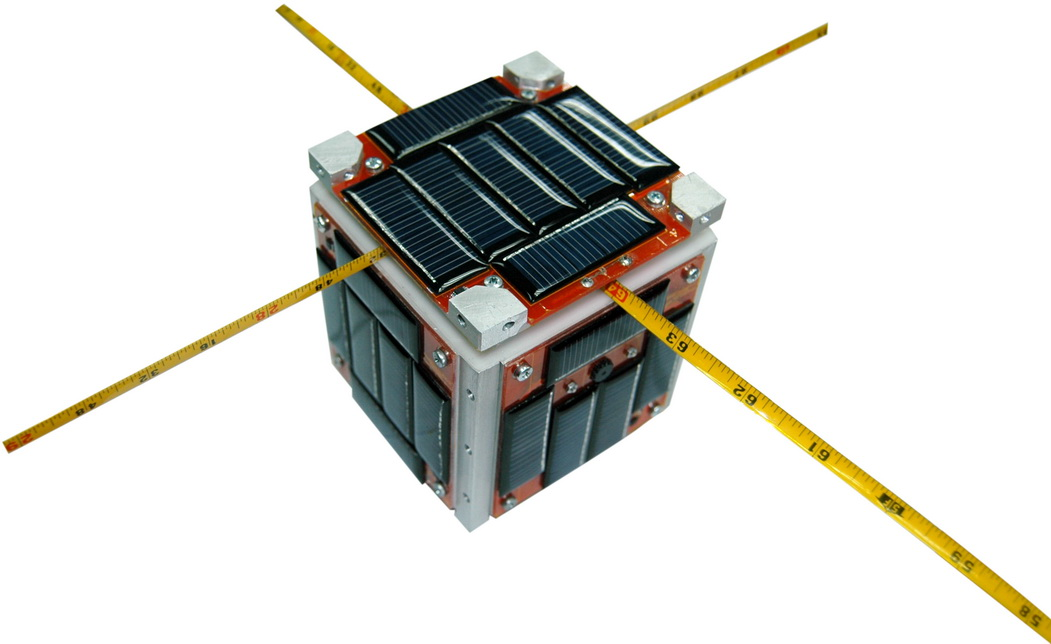
\includegraphics{f1_cubesat_fm}
	\caption{The ``F-1'' CubeSat of the FPT University in Vietnam (1U size)}
	\label{fig:cubesat}
\end{marginfigure}

Given the above, this thesis is focused on the increasingly popular \textbf{nanosatellite} technology \autocite{sweeting_modern_small_2018a}. \textbf{CubeSats}, the most popular class of nanosatellite, were introduced as a concept in 1999. Their low cost and size, as well as their relatively low complexity, have allowed universities and organizations worldwide to launch over 1530 CubeSats by 2021 \autocite{swartwout_cubesat_database_2021}.
	
CubeSats are designed using ``building blocks'' sized at \SI[product-units = single]{10 x 10 x 10}{\centi\metre} called \textbf{Units}. Typical satellite sizes are obtained by ``stacking'' these units, resulting in satellites of 1U, 1.5U, 2U, 3U, 6U and 12U. Each unit can weigh up to \SI{2}{\kilogram} \autocite{CDS14}. Internally,  CubeSats use low-cost commercial electronic components, henceforth referred to as \textbf{\acf{COTS}} components. CubeSats are typically launched in Low Earth Orbits (\acs{LEO}) \autocite{anthopoulos_orbital_analysis_2020,riebeek_catalog_earth_2009}, deployed as secondary payloads in larger satellite launches (``piggyback launches''), and often remain active for periods of about 1 to 3 years.

\pagebreak[4]
\section{Thesis goals \& contribution}

\begin{marginfigure}
	\centering
	\begin{tikzpicture}[every node/.style={scale=0.8}]
	\pie[
	sum=auto,after number=,radius={1},text=pin,rotate=0,scale font,color={MaterialGreen400, MaterialBlue, MaterialAmber, MaterialRed, MaterialYellow, MaterialGrey}
	]{131/Mission complete,
		144/In progress,
		61/Early loss,
		120/\acs{DOA},
		37/{Failed launch},
		204/Unknown
	}
	
	\end{tikzpicture}
	\caption[CubeSat mission status since 2000]{CubeSat mission status since 2000 \autocite{swartwout_cubesat_mission_2019}}
			\label{fig:cubesat_status}
			\acusepage{reliability}
		\end{marginfigure}
		
		\begin{marginfigure}
			\centering
			\begin{tikzpicture}[every node/.style={scale=0.8}]
			\pie[
			sum=auto,after number=,radius={1},text=pin,rotate=0,scale font,color={MaterialGreen400, MaterialBlue, MaterialAmber, MaterialRed, MaterialYellow, MaterialGrey}
			]{38/Mission complete,
				54/In progress,
				34/Early loss,
				88/\acs{DOA},
				17/{Failed launch},
				58/Unknown
			}
			
			\end{tikzpicture}
			\caption[CubeSat mission status from independent manufacturers]{CubeSat mission status from ``hobbyists'' (scientific and other research/educational projects) \autocite{swartwout_cubesat_database_2021}}
			\label{fig:cubesat_status_hobbyist}
		\end{marginfigure}
	
% Some breathing space after the figures
\marginpar{\vspace{1cm}}

This work is dedicated to improving the reliability of nanosatellites and CubeSat systems. Although the majority of large satellite launches have completed their missions even partially \autocite{kattakuri_failures_spacecraft_2019,jacklin_smallsatellite_mission_2019}, 39.6\% of launched CubeSats have failed to complete their mission or did not operate at all. This number can be increased to 57.0\% if we focus on the subset of CubeSats launched as the first space mission of an organisation lacking the expertise of major manufaturers and space entities.

The reasons explaining the high failure rate of CubeSats are mainly related to the compressed manufacturing schedule, which leads to errors and problems that are not detected during design. Sources of failures such as environmental degradation (thermal cycles, radiation), lack of safety margins in power and telecommunications, and software problems, combined with the general lack of experience and haphazard procedures followed by new manufacturers, reduce the overall reliability of nanosatellites \autocite{swartwout_cubesat_mission_2019,langer_reliability_estimation_2017}.

The approaches taken to increase CubeSat reliability include:
\begin{compactitem}
	\item Reducing the number of potential failures from the design phase, by including reliability analysis in the early phases of a project
	\item Structured reliability assessment and improvement tools, such as \textbf{\acf{FMEA}} and \textbf{\acf{FDIR}} \autocite{faure_lean_satellites_2017,menchinelli_reliability_engineering_2018}
	\item Adaptation and adoption of open space standards for design, manufacturing and verification
\end{compactitem}


This work intends to supplement the toolbox of CubeSat manufacturers, by detailing a structured approach to \ac{FDIR} based on the \textbf{European \acs{ECSS} standards} and the work of the \textbf{\acs{SAVOIR}} initiative\footurl{https://savoir.estec.esa.int} of the European Space Industry. In the main matter, we will discuss how these ideas can be adapted to a low-scale CubeSat mission, presenting:
\begin{itemize}
	\item A structured method to investigate the possible failure modes of a satellite, and how they can be tackled
	\item Software that can respond to and safely manage all critical in-orbit failures
	\item A \textbf{configurable and modular} architecture that allows operators to easily modify the behaviour of the \acs{FDIR} system and tailor it for different environments.
\end{itemize}

\begin{figure}
	\centering
	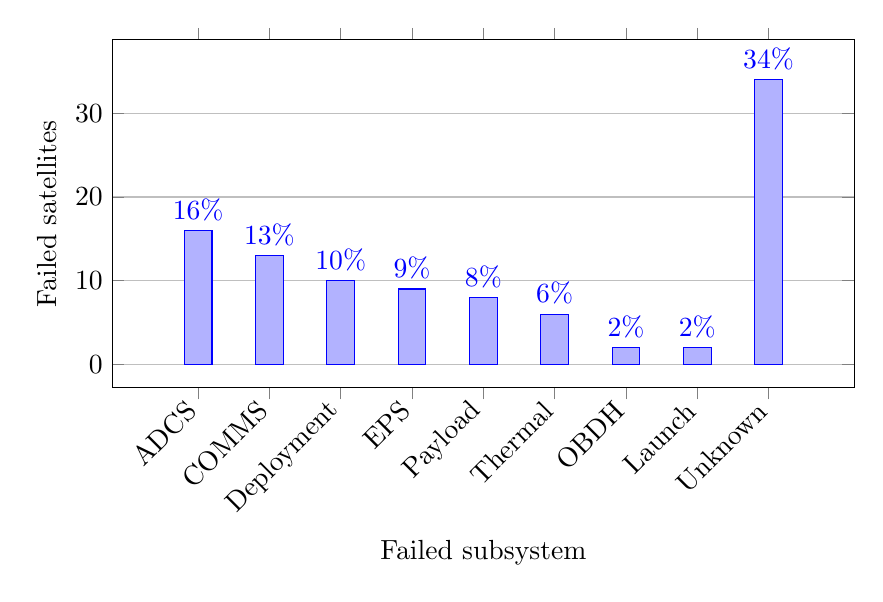
\begin{tikzpicture}
	\begin{axis}
	[
	ybar,
	enlargelimits=0.15,
	ylabel={Failed satellites}, % the ylabel must precede a # symbol.
	xlabel={Failed subsystem},
	symbolic x coords={ADCS, COMMS, Deployment, EPS, Payload, Thermal, OBDH, Launch, Unknown}, % these are the specification of coordinates on the x-axis.
	xticklabels={ADCS, COMMS, Deployment, EPS, Payload, Thermal, OBDH, Launch, Unknown},
	xtick=data,
	nodes near coords, % this command is used to mention the y-axis points on the top of the particular bar.
	nodes near coords align={vertical},
	ymajorgrids={true},
	width=11cm,
	height=6cm,
	x tick label style={rotate=45,anchor=east},
	nodes near coords={\pgfmathprintnumber\pgfplotspointmeta\%}
	]
	\addplot coordinates {(ADCS, 16) (COMMS, 13) (Deployment, 10) (EPS, 9) (Payload, 8) (Thermal, 6) (OBDH, 2) (Launch, 2) (Unknown, 34) };
	
	\end{axis}
	\end{tikzpicture}
	\caption[Main CubeSat failure causes]{Main CubeSat failure causes (\(n=50\)) \autocite{bouwmeester_survey_implementation_2017}}
	\label{fig:whyfail}
\end{figure}

The proposed \acs{FDIR} system aims to increase confidence during development, but also to quickly incorporate new information generated during testing, or even after launch.

In addition to the presentation, analysis and commentary on the standards, this thesis focuses on the application of the aforementioned \acs{FDIR} structure to the \emph{AcubeSAT} nanosatellite, and includes an experimental implementation of the \acs{FDIR} suite in hardware \& software.

\section{Thesis structure}

This document begins with a summary of the AcubeSAT mission, which is the main motivation behind it (\Cref{cap:acubesat}). It then proceeds to an analysis of the main \acs{FDIR} standards and philosophy, focusing on the parts of particular importance to CubeSats and educational missions (\Cref{cap:savoir}). The next section discusses the application of the previous standards to the design of AcubeSAT, and analyses some design decisions and implementation details of \acs{FDIR} on the nanosatellites (\Cref{cap:acufdir}).

The last chapter includes a practical demonstration of the proposed \acs{FDIR} on a simple two-sensor test system (\Cref{cap:practical}). The system is constructed so that it can detect and recover from all foreseen possible failures, using software libraries covering the \acs{ECSS} and \acs{FDIR} standards. After the system has been developed, a full test of its response to failures is performed. This simulation platform is configured to emulate the satellite system, including the microcontroller and the ground station.

\chapter{The AcubeSAT mission}
\label{cap:acubesat}

\begin{marginfigure}
    
\includegraphics{acubesat_patch}
    \caption{AcubeSAT mission patch}
\end{marginfigure}

\begin{marginfigure}
    \centering
    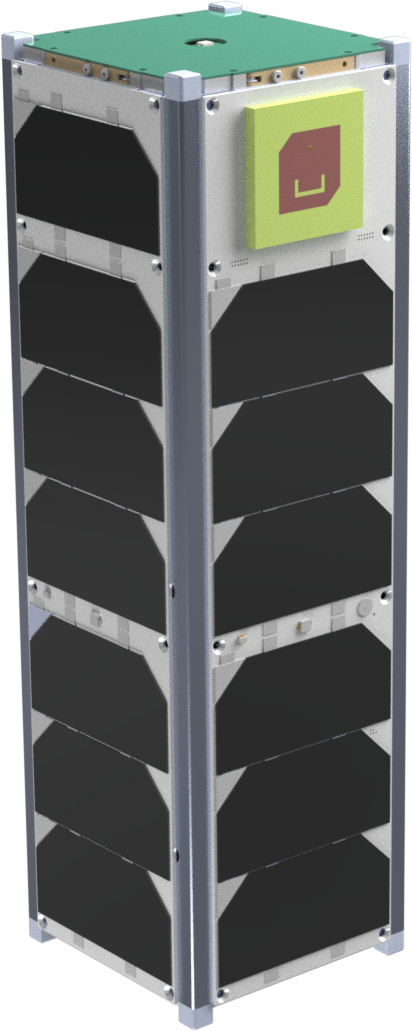
\includegraphics[width=.8\textwidth]{acubesat}
    \caption{AcubeSAT nanosatellite render}
\end{marginfigure}


The implementation framework of this work is the \textbf{``AcubeSAT''} nanosatellite project, which, as of 2021, is under development by students of the Aristotle University of Thessaloniki, and aims to perform biology-centred research in space.

The project was initiated in 2016. In February 2020, it became part of the \foothref{https://www.esa.int/Education/CubeSats_-_Fly_Your_Satellite}{``Fly Your Satellite!\ 3''} programme by the European Space Agency, aiming for a 2023 launch.

AcubeSAT is three CubeSat units large (3U), measuring \linebreak[4]\SI[product-units = single]{10 x 10 x 34.05}{\centi\metre} and weighing \SI{4.26}{\kilo\gram}. Physically, the CubeSat contains the \textbf{experimental payload}, covering the bottom 2U, and the rest of the \textbf{spacecraft platform} which takes up the remaining 1U.

The AcubeSAT project follows an \textbf{open-source philosophy}, making its software, developments and documentation available to the public under free licenses, at \url{https://gitlab.com/acubesat/}.

\section{The mission}

AcubeSAT's main mission is the study of \textbf{eukaryotic cells} in \acl{LEO}, and more specifically the assessment of the effects of \emph{radiation} and \emph{microgravity} on 190 different strains of the yeast species \emph{Saccharomyces Cerevisiae}. The previous are achieved with a novel lab-on-a-chip construction, structured around a \textbf{microfluidic chip} (\Cref{fig:microfluidic_chip}) \autocite{volpetti_microfluidic_biodisplay_2017} that allows the regulation of gene expression to be monitored in an unprecedented scale.

The results of the experiment are telemetered to Earth in the form of photographs, where the entirety of the microfluidic chip's chambers are depicted, and results are extracted acording to the \textbf{fluorescence level} produced in each chamber. The results in orbit are compared to a similar ground-based reference experiment.

\begin{figure}[t]
	\centering
	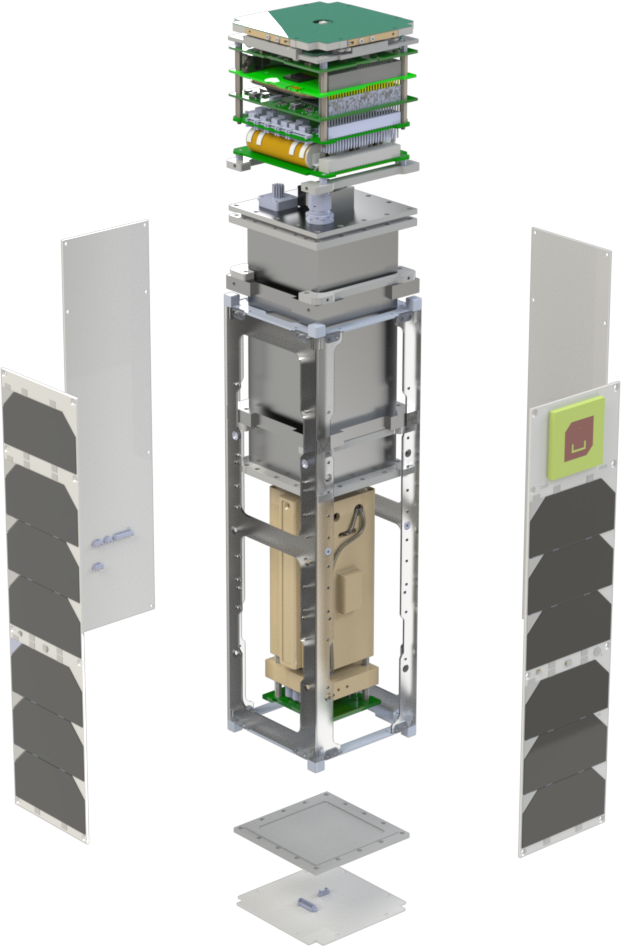
\includegraphics[width=.7\textwidth]{cubesat_exploded}
	\caption{View of AcubeSAT's interior, showing the different subsystems and the experimental setup}
\end{figure}

\section{Subsystems}

The AcubeSAT nanosatellite is technically and programmatically split into 11 different subteams or \textbf{subsystems}, each responsible for a different section of the satellite, and made up out of \SIrange{2}{9}{} dedicated members.

\begin{marginfigure}
	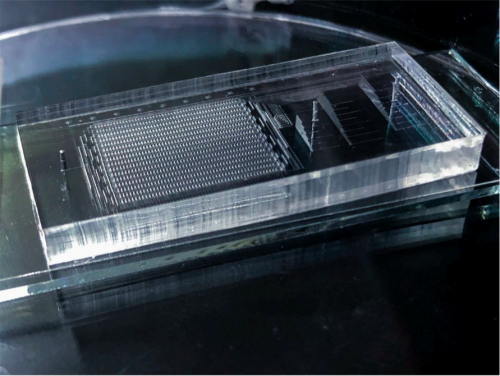
\includegraphics{microfluidic_chip}
	\caption{Microfluidic chip engineering model}
	\label{fig:microfluidic_chip}
\end{marginfigure}

In the following sections, a brief introduction on the function and design of each subsystem is presented. As the Systems Engineering and \acl{PA} process is inherently connected to the function of all subsystems, the details relevant to \acs{FDIR} are also mentioned. For more detailed information, the reader is encouraged to refer to \foothref[,]{https://acubesat.spacedot.gr/subsystems/}{AcubeSAT's website} or to the publicly available \foothref[.]{https://gitlab.com/acubesat/documentation/cdr-public}{\ac{CDR} documents}
\subsection{\acf{ADCS}}
\label{sec:adcs}

The \ac{ADCS} subsystem is responsible for controlling the \textbf{attitude} and orientation of the spacecraft in orbit. This is achieved using a series of \ac{COTS} control actuators (one 3-axis magnetorquer board, one 1-axis reaction wheel), sensors for attitude determination (1 gyroscope and 2 magnetometers), and filtering, determination \& control algorithms \autocite{DDJF_AOCS}.

The \ac{ADCS} can operate under different \textbf{pointing profiles} for different attitude needs:
\begin{enumerate}
	\item \textbf{Detumbling}, where the satellite is attempting to minimize its angular acceleration, to ensure a stable communications link, prevent detachment of parts and allow easier regaining of pointing.
	
	\begin{marginfigure}
		\centering
		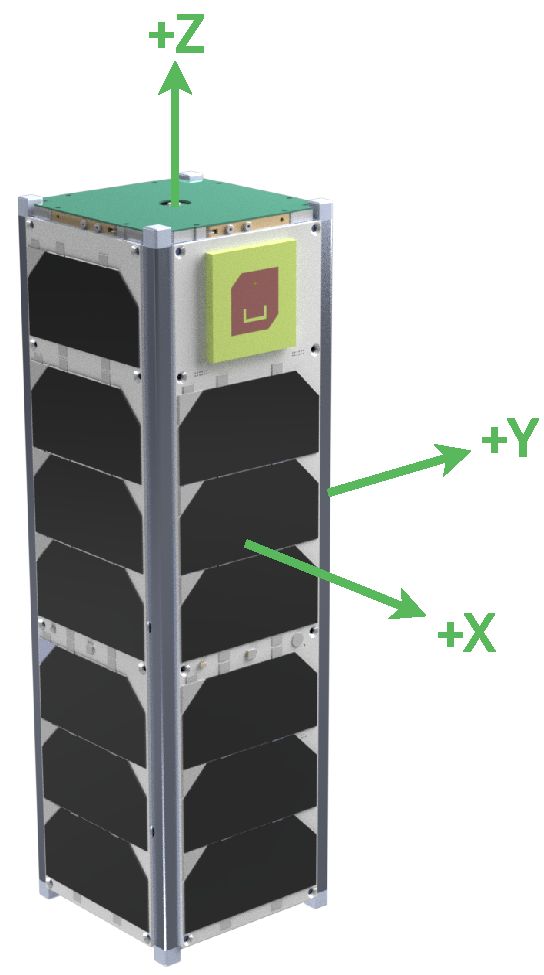
\includegraphics[width=.7\textwidth]{AcubeSAT_reference_frame_cropped.pdf}
		\caption{AcubeSAT reference frame}
		\label{fig:frame}
	\end{marginfigure}
	
	Detumbling mode is implemented in the simplest possible way, using only one of the 2 redundant magnetometers and a simple control algorithm. It is activated when there is no need to apply any of the specific pointing modes, or if the spacecraft angular rate is too high. In AcubeSAT, system-wide \emph{Safe Mode}, \emph{Commissioning Mode} and \emph{Science Mode} adopt detumbling.
	
	\item \textbf{Nadir pointing}, where the satellite points the \(+X\) side towards the Earth. This profile is used during \emph{Nominal Mode} on passes over the \acl{GS}, where the directional patch antenna needs direct visibility.
	
	\item \textbf{Sun pointing}, where the satellite points two sides to the sun, each with a \SI{45}{\degree} angle of incidence, in order to maximise solar panel input. This profile is used during \emph{Nominal Mode}, between \ac{GS} passes, in order to ensure a positive power budget.
\end{enumerate}

\begin{margintable}
	\centering
	\caption[Maximum ADCS error values after stabilisation]{Maximum \ac{ADCS} error values after stabilisation}
	\label{tab:adcsape}
	\begin{tabular}{@{}ll@{}}
		\toprule
		Error                      & Value                    \\ \midrule
		Absolute Performance Error & \( < \SI{30}{\degree} \) \\
		Absolute Knowledge Error   & \( < \SI{1}{\degree} \) 
	\end{tabular}
\end{margintable}

The performance of the \ac{ADCS} system can be summarised using performance metrics such as the ones presented in \Cref{tab:adcsape}.

\subsection{\acf{COMMS}}

The communications subsystem is responsible for transmitting data between the Earth and the spacecraft in orbit. The transmitted data is split into 3 different categories \autocite{DDJF_TTC}:
\begin{itemize}
	\item \textbf{\acf{TC}}: Commands from the Earth to the satellite. They can be used to request information, or to perform specific spacecraft actions.
	\item \textbf{\acf{TM}}: Information sent from the satellite towards Earth, typically including vital information such as sensor values, system status, timestamps and events.
	\item \textbf{Science data}: The scientific data generated by the payload. These are the highest-volume data and represent the main scientific output of the mission (i.e.\ fluorescence photographs).
\end{itemize}

It is important to mention that the satellite orbit only allows for a very short visibility duration every day, increasing the needs for on-board autonomy and the importance of a correctly implemented \acs{FDIR} method.

\begin{marginfigure}
	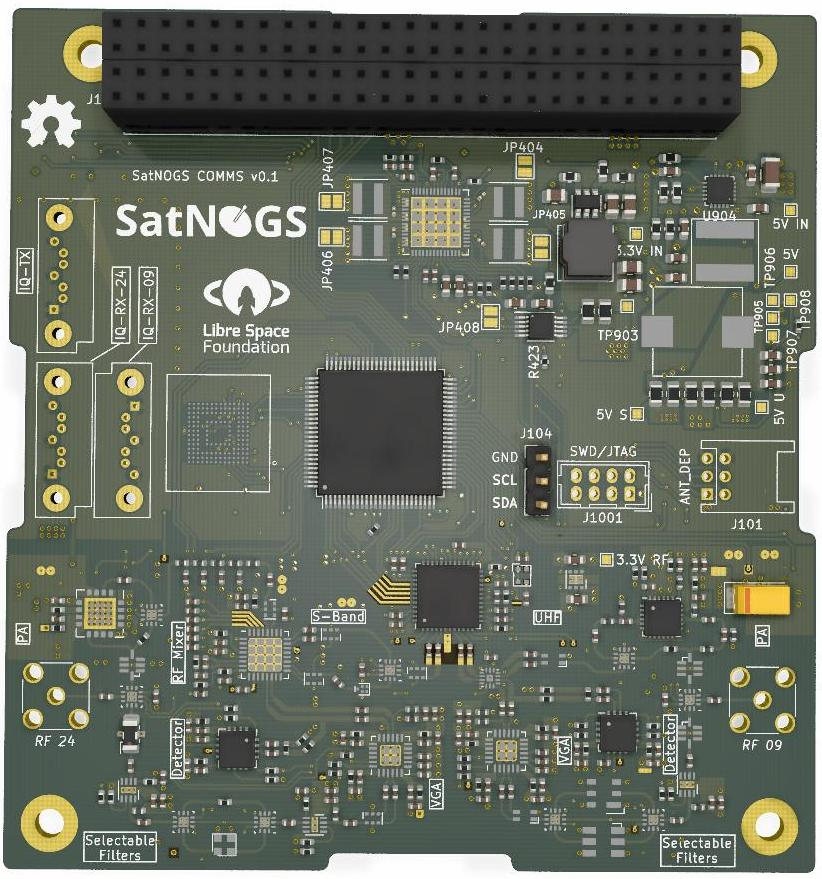
\includegraphics{satnogs-comms}
	\caption{The SatNOGS COMMS board}
\end{marginfigure}

The main component of the \acs{COMMS} subsystem is the \textbf{SatNOGS COMMS board} \autocite{surligas_satnogscomms_2021}, an open-source \acs{RF} transceiver developed by the \href{https://libre.space/}{LibreSpace Foundation}, based on \acs{CCSDS} telecommunications standards.

Communication takes place using 2 frequency bands on the \acs{ISM} range, namely \SI{436.5}{\mega\hertz} and \SI{2.425}{\giga\hertz}, supported by a deployable turnstile and a directional patch antenna respectively. The use of \acs{ISM} frequencies allows easy radio-amateur access to the satellite. The first (\acs{UHF}) band also emits a periodic \textbf{beacon}, listing information about satellite status.

The communications subsystem is also responsible for the \ac{EMC} analysis and interference mitigation, as well as the design and construction of the satellite \acl{GS}. The \acl{GS} will be part of \textbf{SatNOGS} \autocite{white_overview_satellite_2018}, a global network of satellite ground stations based on open technologies and open data.

\subsection{\acf{EPS}}
The \ac{EPS} is the subsystem responsible for the generation, distribution and storage of electrical power of the spacecraft. It is a critical aspect of the spacecraft due to the direct dependence of all subsystems to it, and is theorised to be one of the most common reason for CubeSat failure \autocite{langer_reliability_cubesats_2016,bouwmeester_survey_implementation_2017}.

\begin{margintable}
	\caption{AcubeSAT nominal mode power budget}
	\label{tab:power_budget}
	\begin{tabularx}{\linewidth}{@{}lX@{}}
		\toprule
		\textbf{Consumer}            & \textbf{Power}            \\ \midrule
		\acs{ADCS}          & \SI{1.10}{\watt} \\
		\acs{COMMS}         & \SI{0.85}{\watt} \\
		\acs{EPS}           & \SI{0.99}{\watt} \\
		\acs{OBC}           & \SI{0.12}{\watt} \\
		\acs{SU}            & \SI{0.25}{\watt} \\ \midrule
		Total               & \SI{3.30}{\watt} \\
		Orbit Average Power & \SI{4.24}{\watt} \\ \bottomrule
	\end{tabularx}
\end{margintable}

AcubeSAT has opted for a \ac{COTS} subsystem approach for the \ac{EPS} \autocite{DDJF_SYS}:
\begin{itemize}
	\item \textbf{Solar panels} are procured from EnduroSat. Four 3U panels cover the \(X\) and \(Y\) faces of the satellite, and one 1U panel covers the \(-Z\) face.
	\item The \textbf{\ac{PCDU}} is procured from NanoAvionics and offers 10 switched channels with overcurrent protection over 4 voltage rails, as well as 4 \ac{MPPT} converters.
	\item The \textbf{battery pack}, also procured from NanoAvionics, contains 4 18650 Li-Ion cells in a 2S2P\footnote{2 series, 2 parallel} configuration.
\end{itemize}



\FloatBarrier
A dynamic approach is taken with regards to power budget calculation:
\begin{compactenum}
	\item The in-orbit power generation is calculated for the duration of the mission using the \textbf{STK} software,\footurl{https://www.agi.com/products/stk} taking into account satellite orientation, pointing profiles and eclipse, with a \SI{1}{\minute} resolution.
	\item The power consumption of the system is calculated on average for each different operational mode.
	\item \acs{MPPT} efficiencies and battery charge level are calculated for each timepoint, assuming worst-case thermal and electrical conditions.
	\item A system-wide 10\% margin is applied to the results.
\end{compactenum}

We have created a Python library consolidating the above steps\footurl{https://gitlab.com/acubesat/eps/power-budget} and producing the necessary outputs to prove the adequacy of the design.

\begin{figure*}[h]
%	\begin{subfigure}[b]{.45\textwidth}
	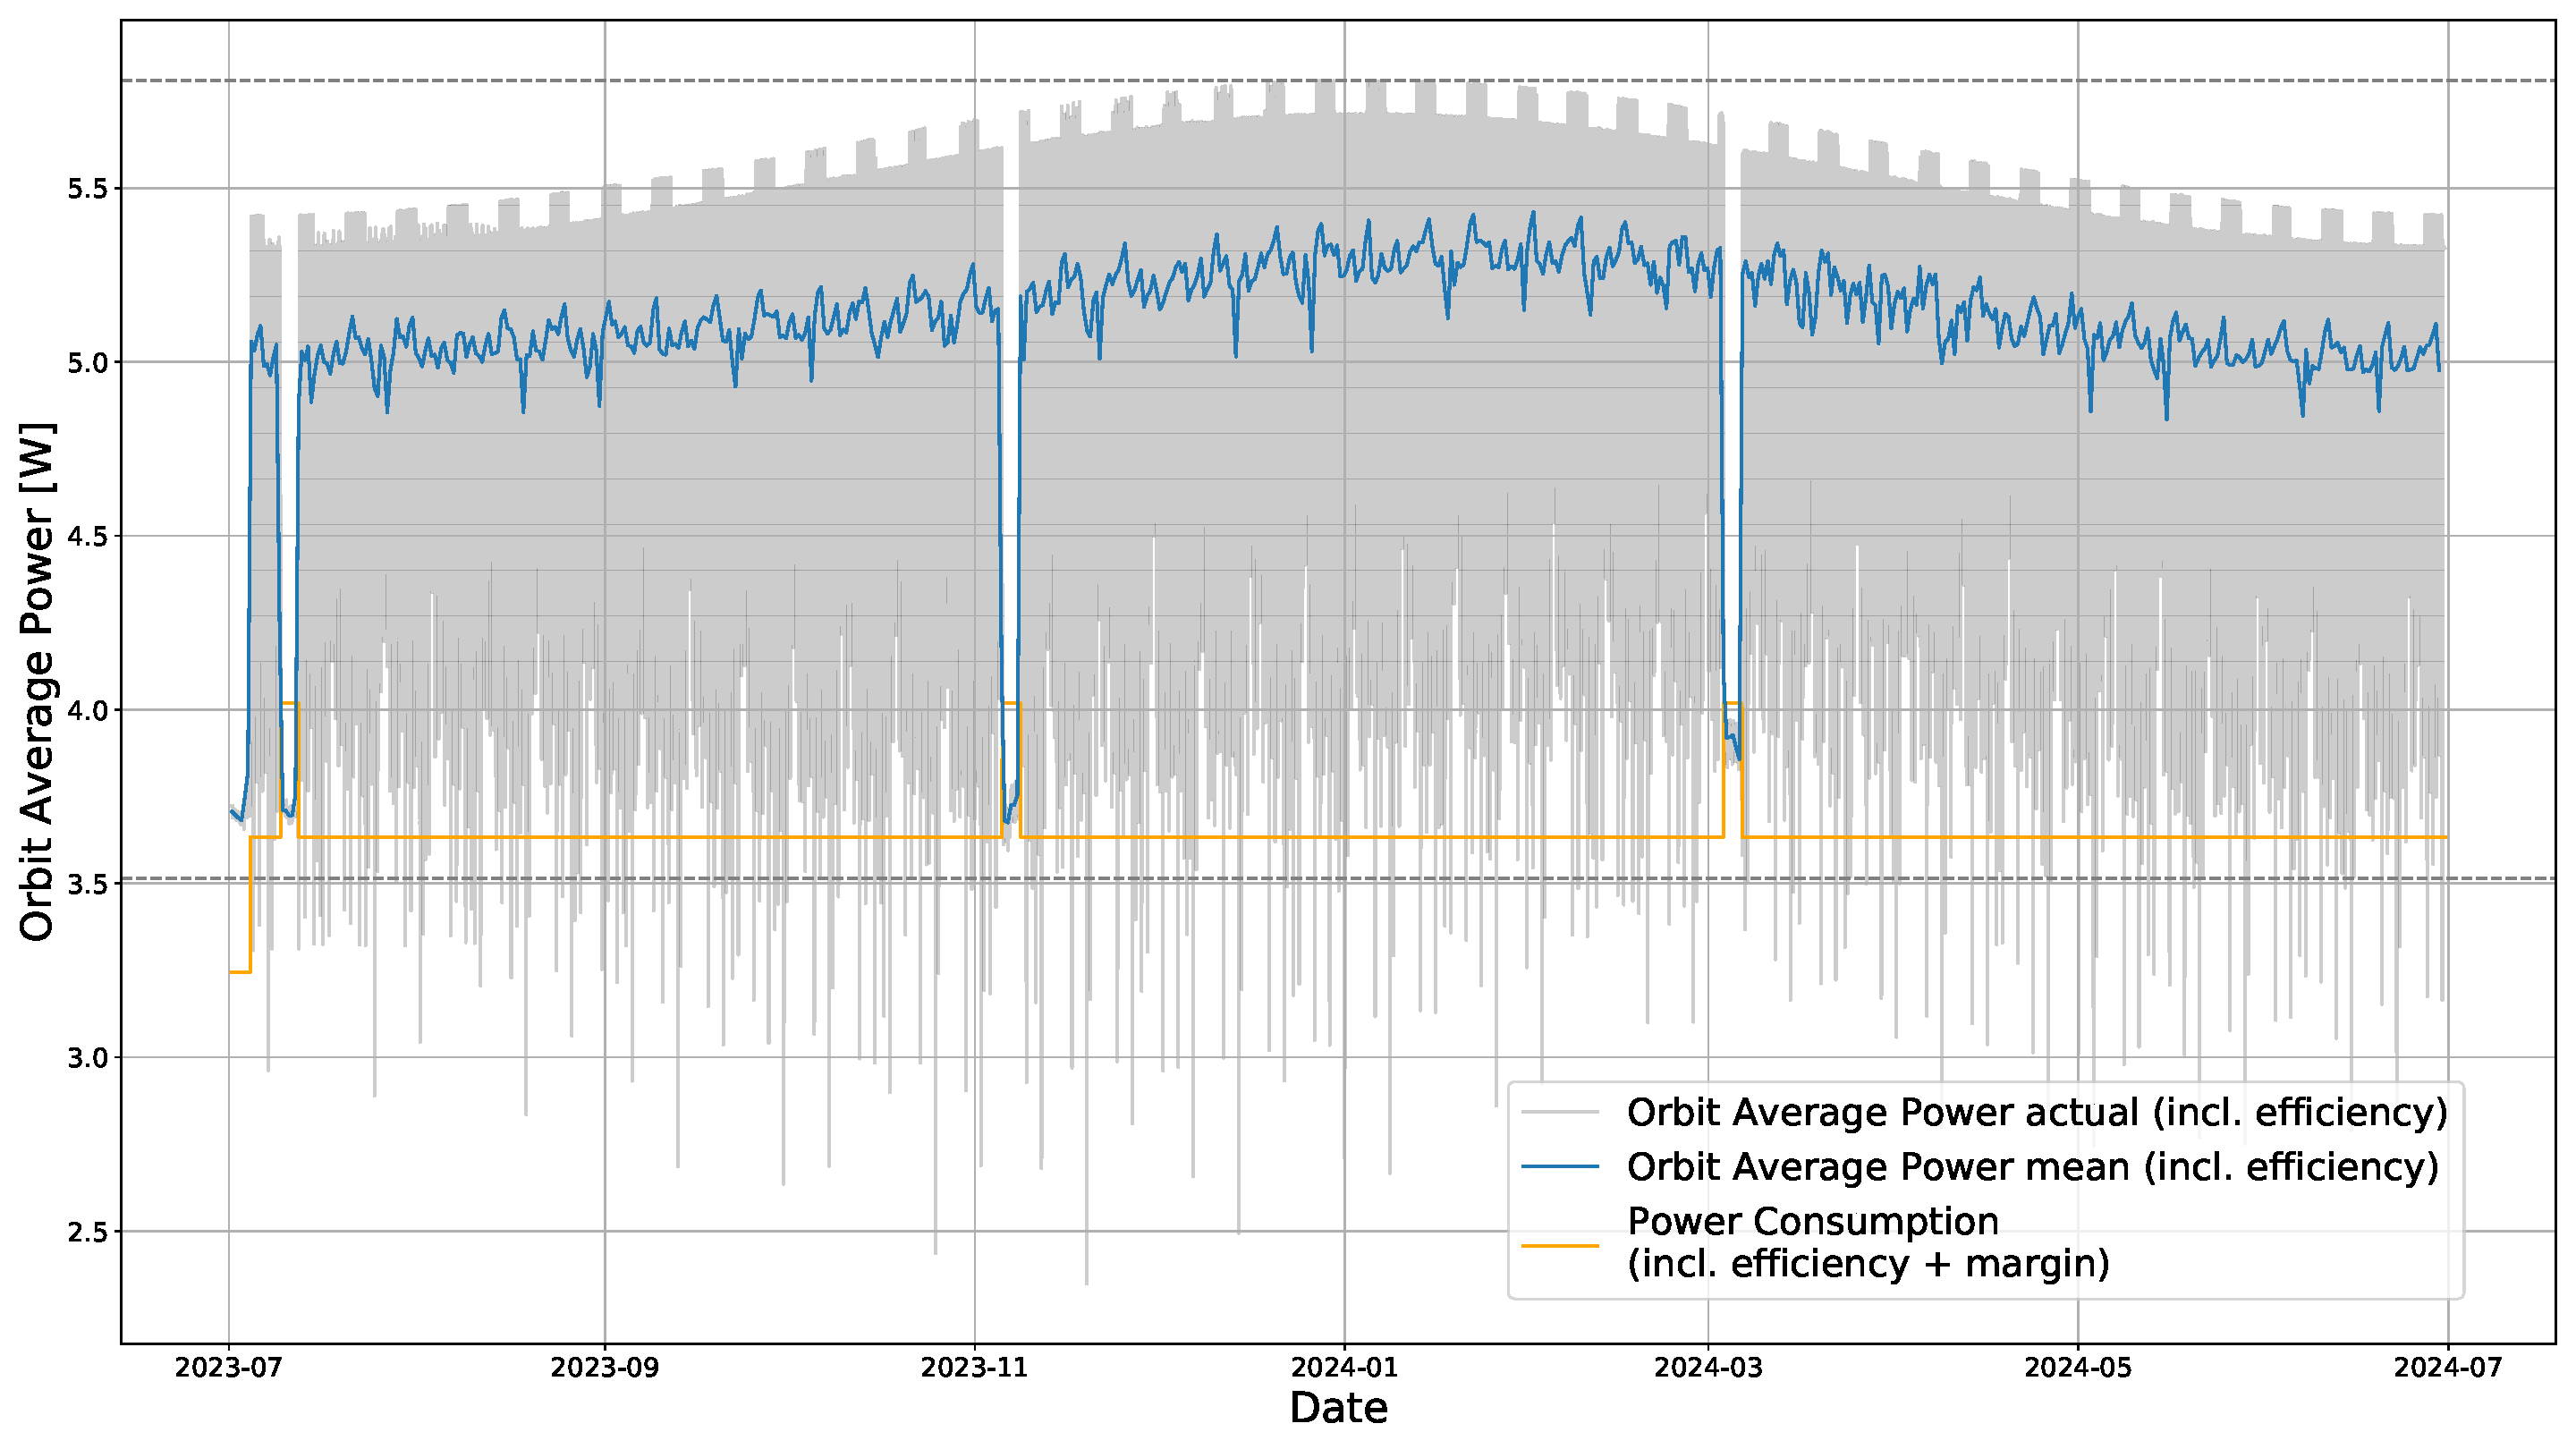
\includegraphics[height=4cm]{Sun Pointing 11:00.total.pdf}
%	\end{subfigure}
	\hfill
%	\begin{subfigure}[b]{.45\textwidth}
	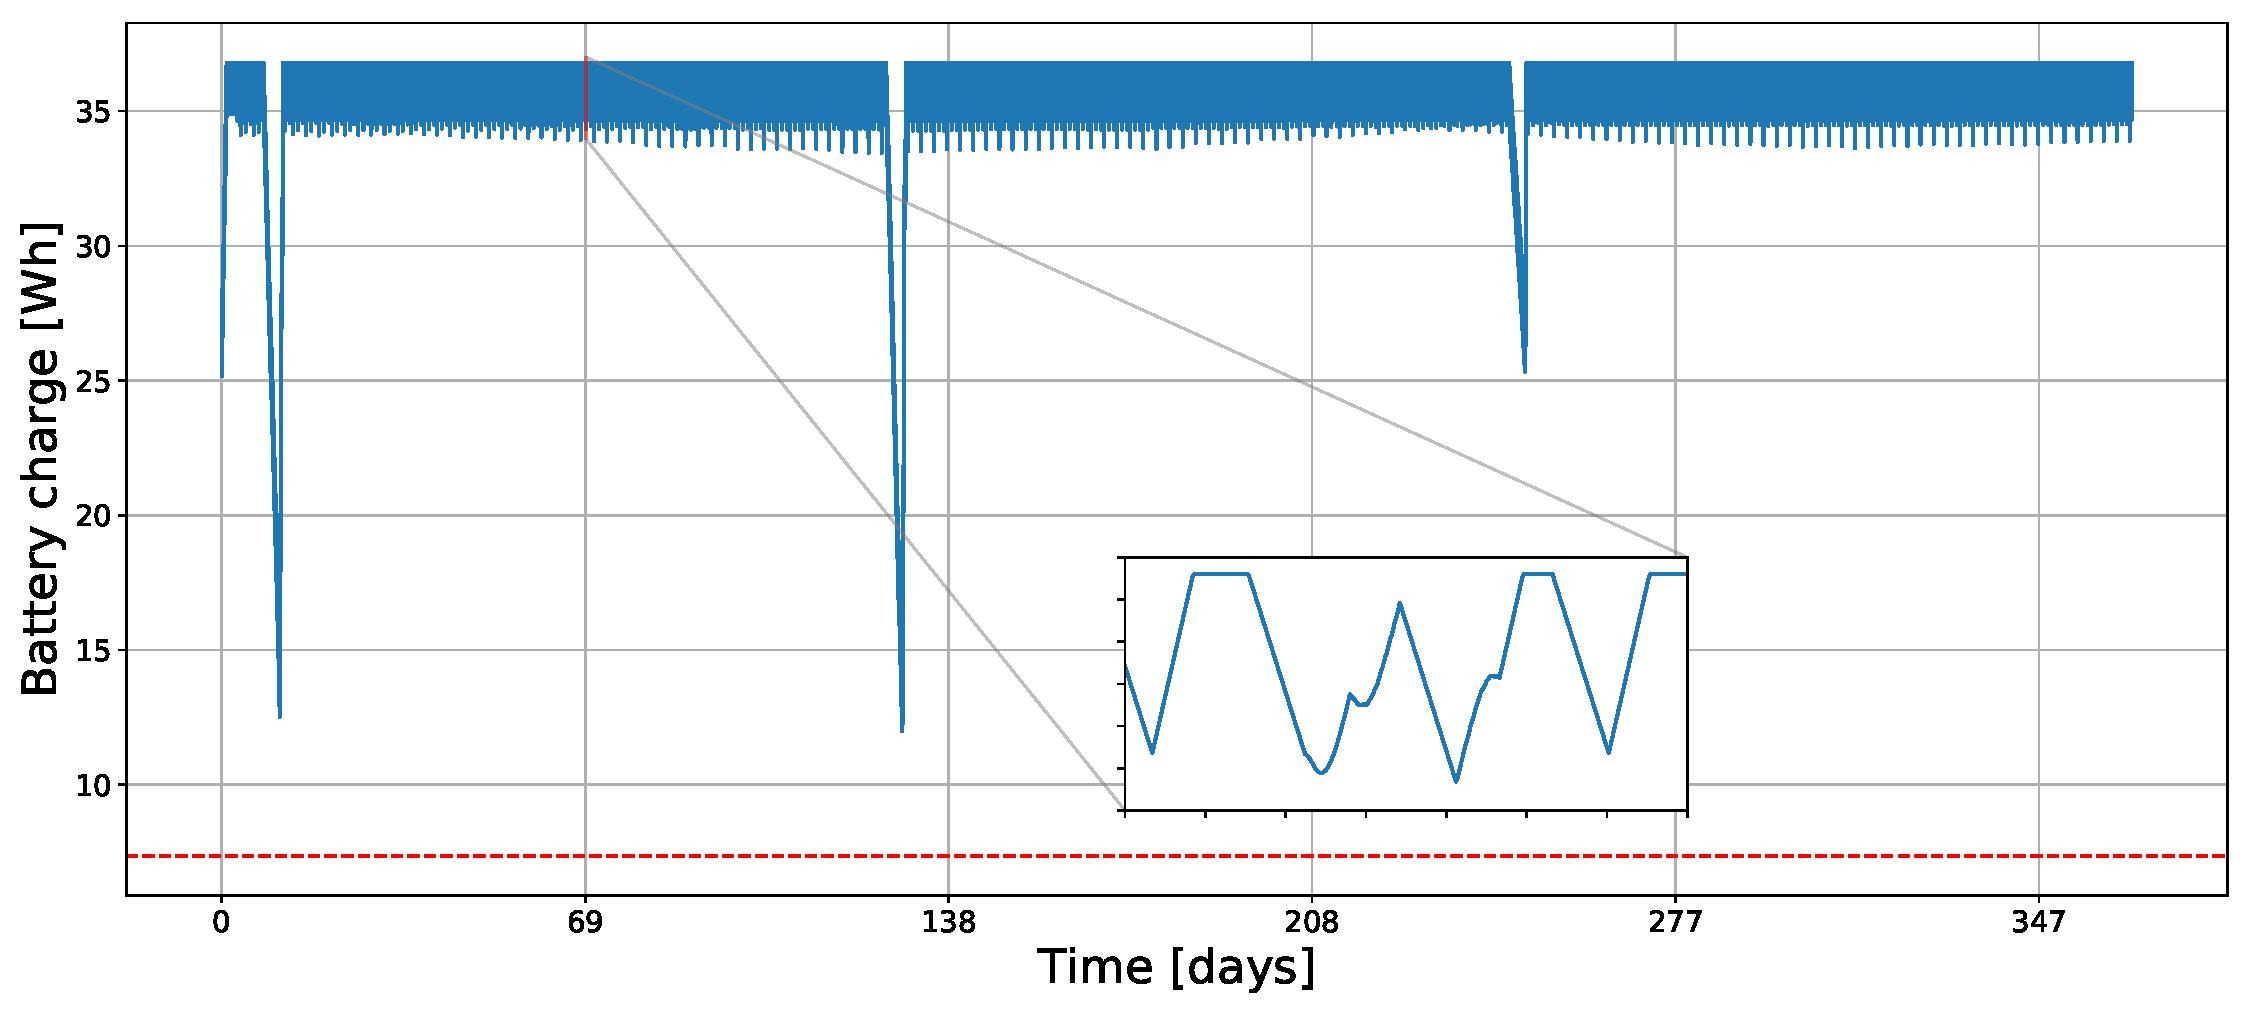
\includegraphics[height=4cm]{Sun Pointing 11:00.discharge.pdf}
%	\end{subfigure}
%	\includegraphics[width=.45\textwidth]{/home/kongr45gpen/Pictures/jeka8ara kapoglis.png}

	\caption[Dynamic power budget analysis]{Dynamic power budget analysis. Left: Power consumption \& generation for the orbit. Right: Battery discharge level throughout the mission.}
\end{figure*}

\subsection{\acf{OBDH}}
\label{sec:obdh}

The \ac{OBDH} subsystem is responsible for the design of the spacecraft's data interfaces, as well as the design of the \textbf{\acf{OBC}} board, tasked with controlling the basic spacecraft functions \autocite{DDJF_OBDH}.

The \ac{OBC} board contains the main \ac{OBC} logic, and is based around a \foothref{https://www.microchip.com/wwwproducts/en/SAMV71Q21RT}{Microchip SAMV71Q21RT} radiation-tolerant microcontroller, and an \acs{MRAM} memory used to store critical data. The board also hosts the in-house components of the \ac{ADCS} subsystem, as a space-saving measure.

\begin{marginfigure}
	\centering
	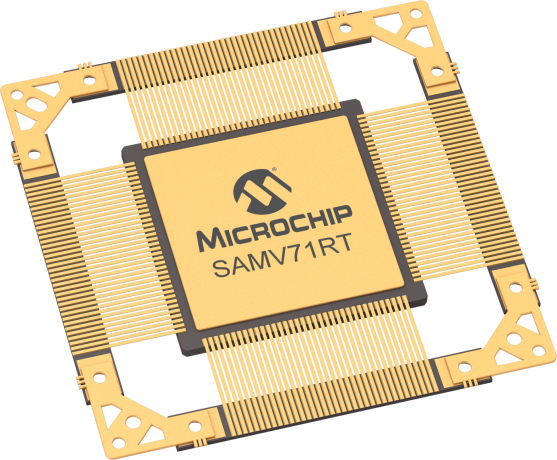
\includegraphics[width=.7\textwidth]{SAMV71Q21RT}
	\caption{The \texttt{SAMV71Q21RT} microcontroller}
	\label{fig:samv71}
\end{marginfigure}

AcubeSAT's data interface is using a cold-redundant \ac{CAN} bus to facilitate cross-subsystem communication, selected due to its robustness and reliability \autocite{bouwmeester_survey_implementation_2017}. AcubeSAT boards implement the PC/104 mechanical interface \autocite{PC104}.

\subsection{\acf{OBSW}}

The \ac{OBSW} subsystem is responsible for the design and development of the nanosatellite's software. The language chosen to be used in the system's 4 \acp{MCU} is a reduced form of \textbf{C++}, and the code is guarded under a number of standards, static checkers and unit tests \autocite{DDJF_OBSW}. All software runs under the Free\acs{RTOS} operating system.



\subsection{\acf{OPS}}

The operations subsystem is responsible for the devising the operational modes \& procedures of the spacecraft, and ensuring the functionality, commandability and observability of the satellite before and during its mission.

During flight, AcubeSAT can remain within one of the following so-called \textbf{system modes} \autocite{MDO}:
\begin{itemize}
	\item \textbf{Launch/Off mode}: During this mode, the satellite is turned completely off, and no subsystems are powered. This is used to represent the state of the spacecraft inside the deployer, where no electronics are allowed to be energised \autocite[req. 3.3.3]{CDS13}, and the CubeSat is in a completely dormant state.
	
	\item \textbf{Commissioning mode}: This mode is initiated as soon as the CubeSat exits the deployer, meaning that launch is complete. It contains the initial boot actions of the spacecraft, including detumbling and antenna deployment. No science takes place during Commissioning mode.
	
	\item \textbf{Nominal mode}: This mode represents the state where the CubeSat will spend most of the time on. Apart from the necessary autonomy functions and battery charging, the CubeSat will also downlink telemetry and science data. No science takes place during nominal mode, except for health checks commanded from the ground. Nominal mode is also the only mode where the satellite performs nadir or sun pointing (\Cref{sec:adcs}).
	
	\item \textbf{Science mode}: This is where the main experiment takes place and payload data are generated. This mode includes operation of the fluidic system, control of the microfluidic chip, reinvigoration of the cells, and periodic acquisition of pictures using the miniaturised microscope.
	
	AcubeSAT has split science mode into \textbf{3 distinct occurrences}, termed sub-experiments \(\alpha\), \(\beta\) and \(\gamma\), lasting 72 hours each, and taking place at different points of the mission to investigate the time-dependence of the observed results.
	
	\item \textbf{Safe mode}: It is common for spacecraft systems to include a \emph{Safe Mode} \autocite[385]{aguirre_introduction_space_2013}, where the spacecraft switches off all non-essential systems and functions, in order to respond to major faults that cannot be corrected by autonomous procedures. Safe mode is intended as a well-defined and well-tested mode which is easy to maintain and reduces risk of any malfunction.
	
	On AcubeSAT, spacecraft functionality in Safe Mode is significantly reduced, and the attitude profile includes detumbling only. However, \ac{UHF} communication and beacon transmission are still active for observability purposes.
\end{itemize}

\begin{table*}[h]
	\centering
	\caption{Overview of AcubeSAT functionality on different modes}
	\label{tab:acubesatmodes}
	\begin{tabular}{@{}llllll@{}}
		\toprule
		Function    & Launch & Commissioning  & Nominal                 & Science        & Safe             \\ \midrule
		\acs{ADCS}  & \color{off} Off    & Detumbling     & \color{on} Pointing                & Detumbling     & Detumbling       \\
		\acs{COMMS} & \color{off} Off    & \acs{UHF} only & \color{on} \acs{UHF} and S-Band    & \acs{UHF} only & \acs{UHF} only   \\
		\acs{EPS}   & \color{off} Off    & \color{on} On             & \color{on} On                      & \color{on} On             & \color{on} On               \\
		\acs{OBC}   & \color{off} Off    & \color{on} On             & \color{on} On                      & \color{on} On             & \color{on} On               \\
		\acs{SU}    & \color{off} Off    & \color{off} Off            & Maintenance \& data only & \color{on} On             & Maintenance only \\ \bottomrule
	\end{tabular}
	\vspace{1em}
\end{table*}


Each mode is associated with a \textbf{functional flow} diagram, showing a high-level description of the spacecraft operation during this mode \autocite{acubesatteam_acubesat_functional_2021}.

\begin{figure}
	\centering
	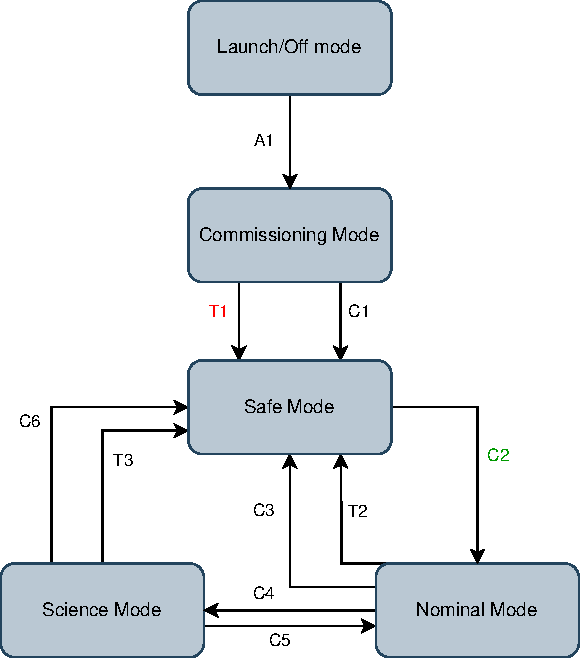
\includegraphics[width=.6\textwidth]{AcubeSAT_System_Modes}
	\caption[][3cm]{All transitions between system modes \parencite{acubesatteam_acubesat_functional_2021}}
	\label{fig:transitions}
\end{figure}


\subsection{Structural}

\begin{marginfigure}[2cm]
	\centering
	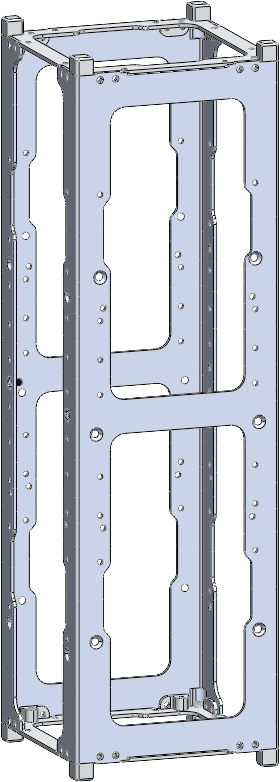
\includegraphics[width=.5\textwidth]{structure}
	\caption{The CubeSat's 3U \acs{COTS} structure}
	\label{fig:structure}
\end{marginfigure}


The Structural subsystem has taken over:
\begin{itemize}
	\item The analysis and configuration of the \ac{COTS} 3-unit structure (\Cref{fig:structure}) housing all the CubeSat's components. Vibration analyses are especially important, as they serve to investigate whether the CubeSat can withstand the launcher's loads.
	\item The complete design, manufacturing and assembly of the \textbf{payload container} and its unibody, hosting the scientific experiment of the mission (\Cref{fig:container}).
\end{itemize}

\subsection{\acf{SYE}}

The \acl{SYE} subteam serves as the technical authority for the satellite. It is responsible for coordinating the developments and interfaces between subsystems, ensuring the conformance to standards and technical requirements, and identifying \& resolving all issues arising from the complex multi-discipline design of the CubeSat.

Additionally, the \ac{SYE} team is responsible for some specific technical developments that do not belong in any of the other subsystems, such as \ac{RAMS}, \ac{FMEA}, harnessing, and the \ac{MAIV} plan.

\subsection{\acf{SU}}
\label{sec:su}
\begin{marginfigure}
	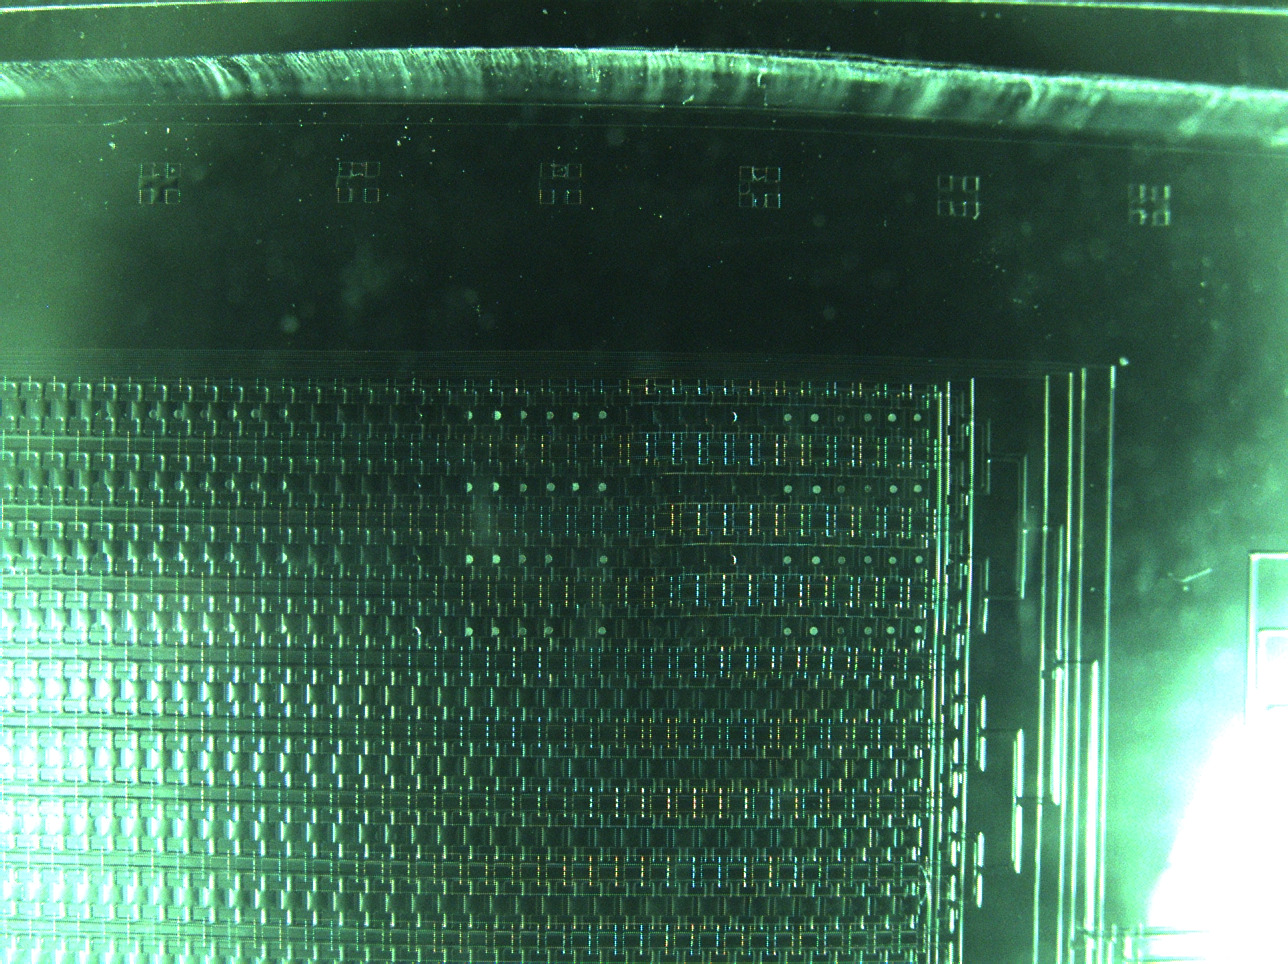
\includegraphics{chipFluor}
	\caption[Example mission image output]{Example mission image output \parencite{DDJF_PL}}
	\label{fig:chip_fluor}
\end{marginfigure}

The \acl{SU} subteam is responsible for the conceptualisation and implementation of the mission's scientific payload, namely the high-throughput study of the effects of \ac{LEO} environments on yeast cells.

The payload is composed of the following functional parts \autocite{DDJF_PL}:
\begin{compactitem}
	\item The \textbf{payload container}, an almost 2U aluminum structure, pressurised at standard atmospheric pressure, and designed to host all the payload instrumentation. The container also accomodates a unibody which mechanically supports all \ac{SU} components.
	\item A \textbf{microfluidic chip} based on \ac{PDMS}, hosting 384 chambers capable of probing 190 distinct strains of \emph{Saccharomyces Cerevisiae} for each subexperiment.
	\item A \textbf{fluidic system} composed from 2 pumps, 8 latching solenoid valves, 6 non-latching solenoid valves, and 3 fluid medium containers
	\item An \textbf{imaging system} operating as a microscope, containing a camera and a series of lights, filters and a lens
	\item A number of \textbf{heaters} to control component operational temperatures
	\item A number of redundant \textbf{sensors} for environmental measurements
	\item A \ac{PCB} containing the microcontroller and rest of the control components of the payload
\end{compactitem}

\begin{marginfigure}
	\centering
	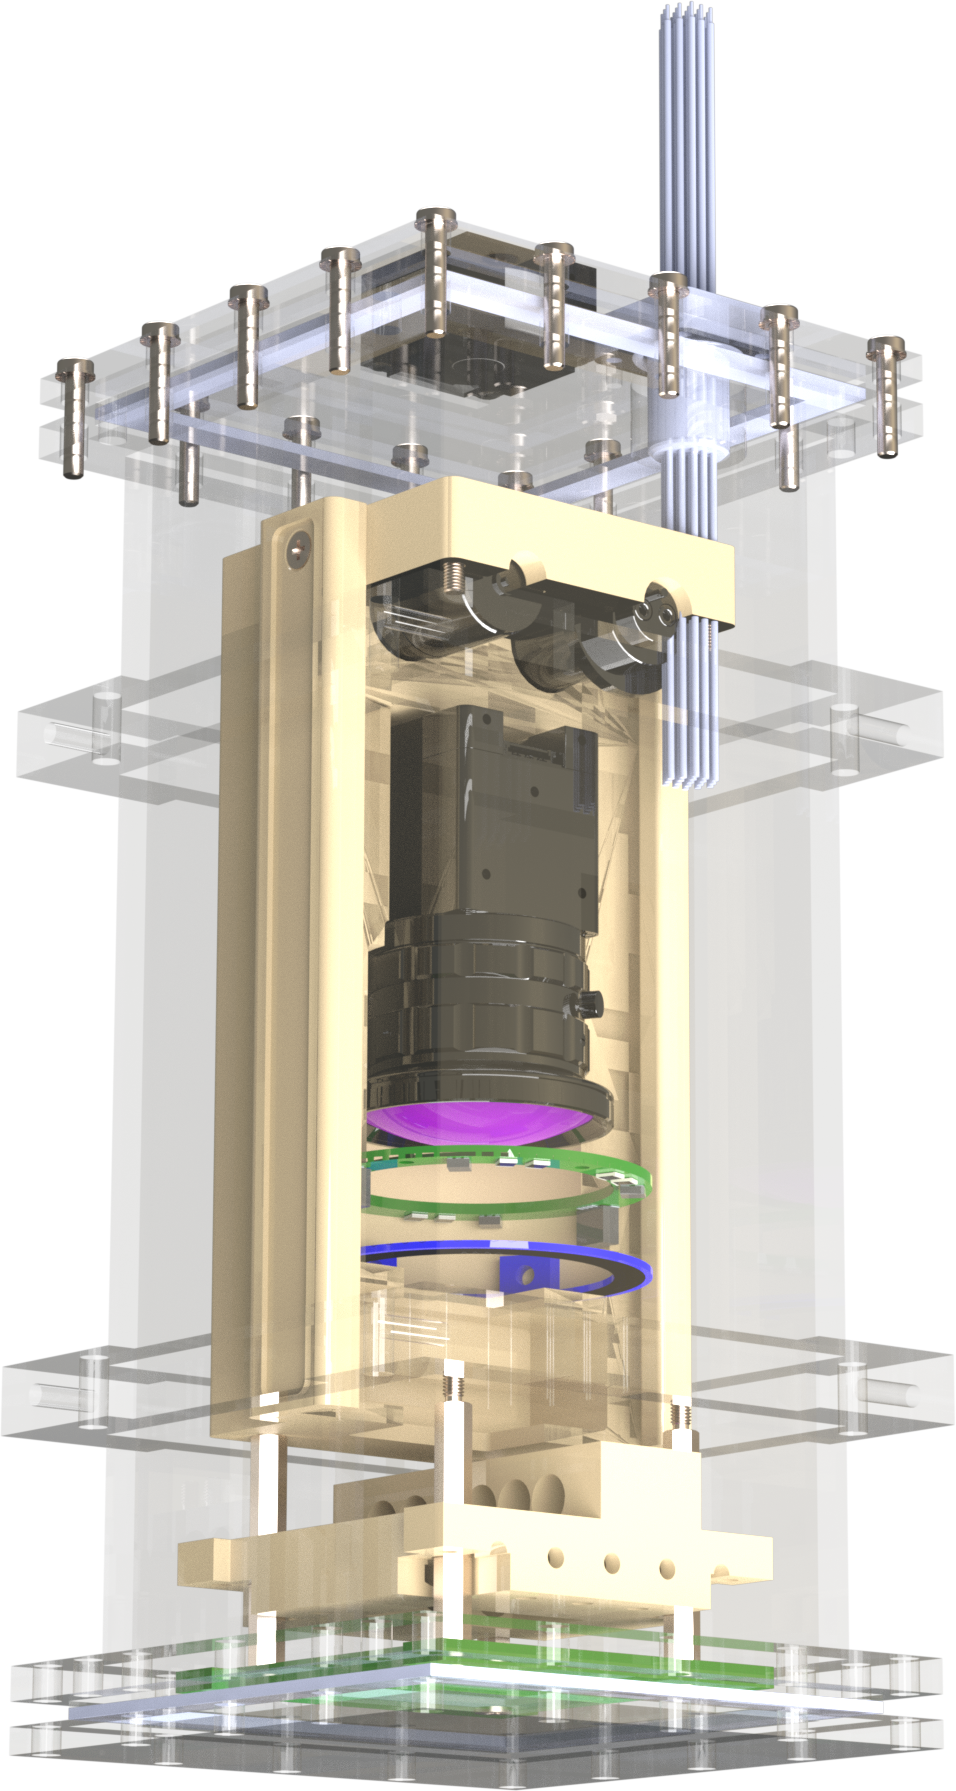
\includegraphics[width=.9\textwidth]{Glass_Payload}
	\caption{Transparent view of the payload container and its internals}
	\label{fig:container}
\end{marginfigure}

\phantomsection\label{sec:su_fdir}
There is a number of constraints that the payload imposes on \ac{FDIR} design:
\begin{enumerate}
	\item \textbf{Interruption} of one of the three 72-hour subexperiments during execution may mean complete loss of the subexperiment. The impact of such an event depends on the duration and timepoint of its occurence. In any case, adequate observability will allow the ground-control experiment to mimic the in-orbit conditions as much as possible.
	\item \textbf{Freezing} of liquids inside the chip and fluidic tubes may lead to permanent damage on the setup. As such, heater operation may be required even during Safe Mode, if the first sub-experiment has been performed and liquid has flown into the system. This characteristic imposes further restrictions on the minimum availability of the system, depending on the thermal conditions.
\end{enumerate}

\begin{figure*}
	\centering
	\caption[The microfluidic chip and its separation into 3 subexperiments and 1 test line]{The microfluidic chip and its separation into 3 subexperiments and 1 test line. The fluid inlets are shown on the left side of the chip, while the outlets are on the right. \emph{Green:} flow layer. \emph{Blue:} control layer.}
	\label{fig:chip}
	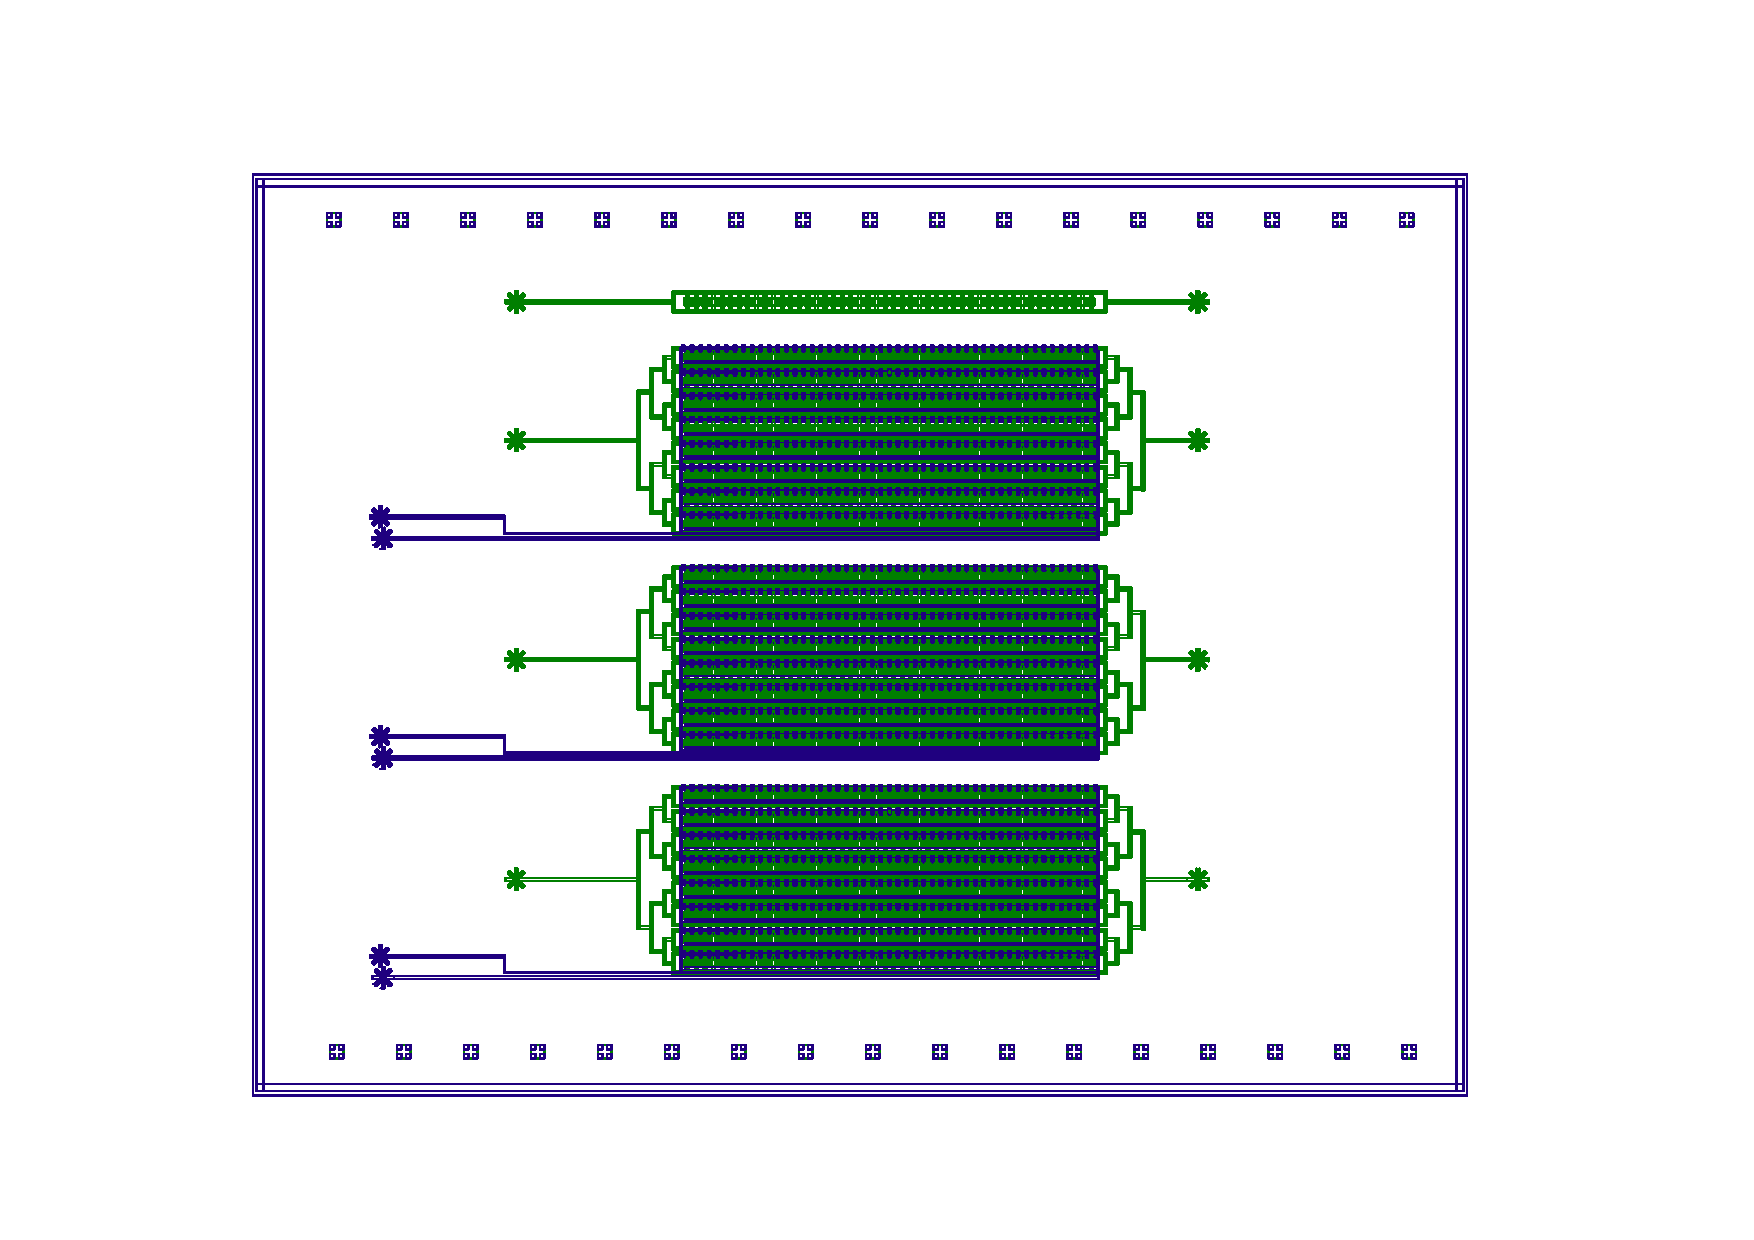
\includegraphics{final_chip.pdf}
	\begin{tikzpicture}[overlay]
	\draw[very thick,dashed,solarized-base01] (5,10.9) rectangle (-7,11.5) node[below right] {Test line};
	\draw[very thick,dashed,solarized-green] (5,7.85) rectangle (-7,10.8) node[below right] {Subexperiment $\alpha$};
	\draw[very thick,dashed,solarized-blue] (5,4.95) rectangle (-7,7.8) node[below right] {Subexperiment $\beta$};
	\draw[very thick,dashed,solarized-red] (5,2) rectangle (-7,4.9) node[below right] {Subexperiment $\gamma$};
	\end{tikzpicture}
\end{figure*}

\subsection{Thermal}

The Thermal subteam is responsible for the thermal analysis of the spacecraft, where the solar and earth albedo conditions are combined with the components' heat dissipation to determine the worst-case temperatures experienced by the satellite in hot and cold conditions.

The results of thermal analysis typically lead to implementation of passive or active thermal control methods. Notably, in AcubeSAT, three electronically-controlled heaters are used for the batteries, \acs{PDMS} chip and valves.

\subsection{Trajectory}

The Trajectory subteam is responsible for the analysis of the spacecraft's orbit, the calculation of radiation effects, the satellite's compliance to space debris regulations, and the estimation of its orbital lifetime.

AcubeSAT's requirements do not dictate use of thrusters, meaning that the satellite's orbit will be determined solely by the launcher, and cannot be altered in flight. As the selected launcher opportunity is unknown until some time before satellite delivery, a number of sensitivity analyses are executed to determine the allowed orbits.

\begin{figure}
	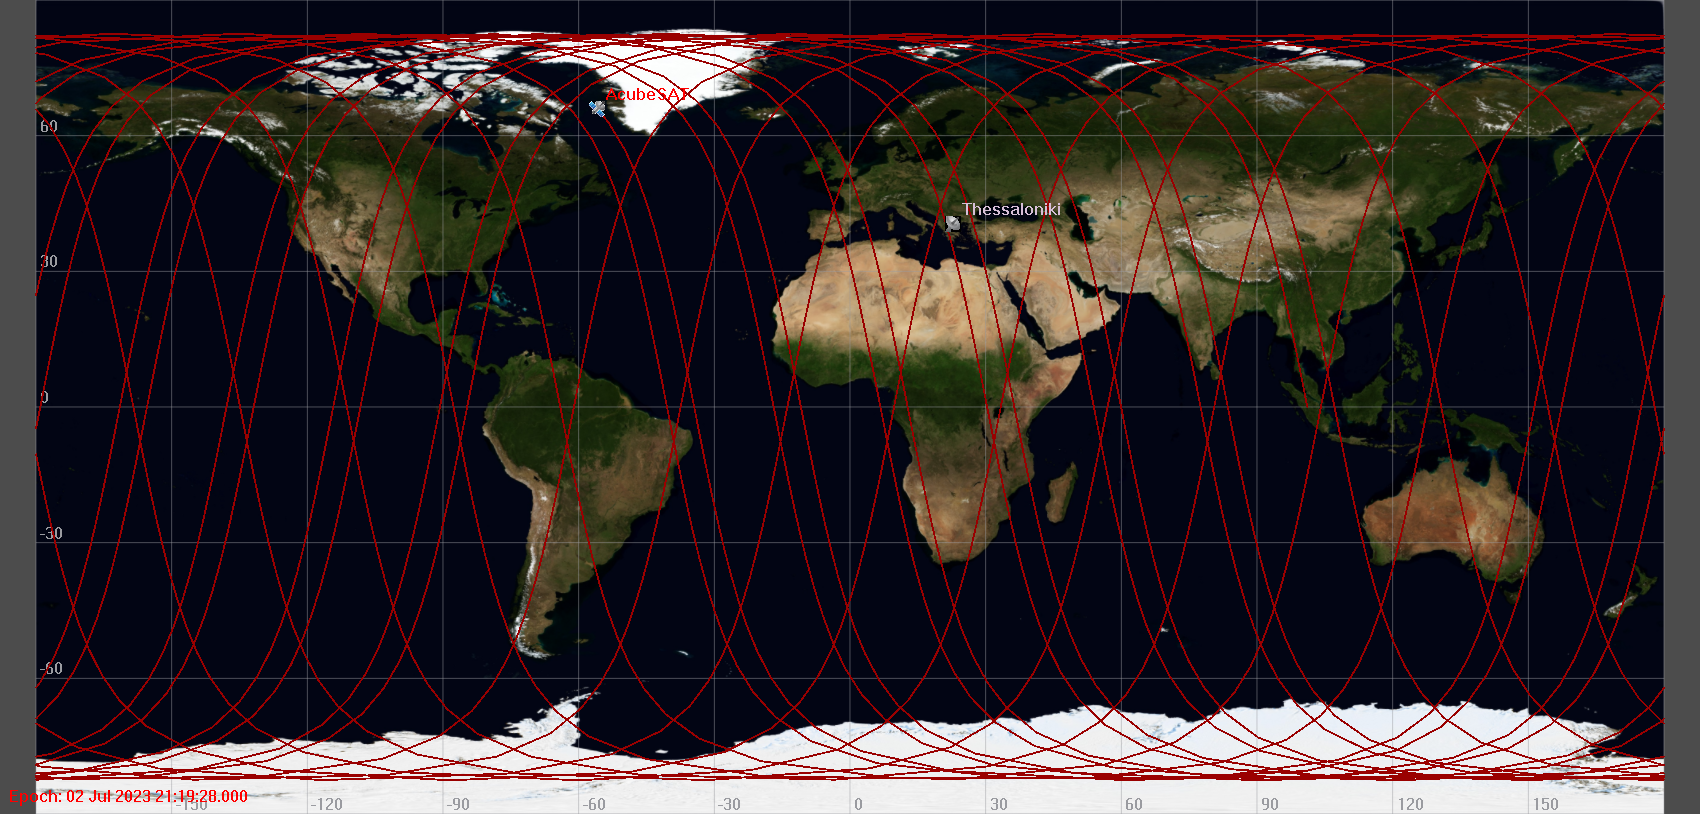
\includegraphics{GmatScreenShot_002}
	\caption[Ground track of an example AcubeSAT orbit, generated using NASA's GMAT]{Ground track of an example AcubeSAT orbit, generated using NASA's \acl{GMAT} \autocite{nasa_general_mission}}
	\label{fig:gmat}
\end{figure}

% Maybe add some info about the sensitivity results and LTAN value?

\section{Tools used}

As a complex project, AcubeSAT uses a set of supporting utilities, ready-made or built by the team, to fulfil its technical and organisational needs. The following tools play a crucial role in the organisation:
\begin{compactitem}
	\item \foothref[,]{https://gitlab.com/acubesat}{GitLab} for sharing code and organizing tasks
	\item \foothref[,]{https://ocdt.esa.int/}{Open Concurrent Design Tool} a platform for sharing technical data and values for satellite components
	\item \foothref{https://www.latex-project.org/}{\LaTeX} and \foothref[,]{https://www.overleaf.com/}{Overleaf} for writing technical literature and documentation
	\item \foothref[,]{https://acubesat.spacedot.gr/requirements-tree}{Requirements Tree} an interactive view of the technical specifications of the satellite
	\item \foothref[,]{https://gitlab.com/acubesat/utilities/mattermost-documentation-bot}{Documentation List} a platform for cataloguing and navigating the documents produced by the team
\end{compactitem}

\end{comment}

\chapter{The SAVOIR \ac{FDIR} concept}
\label{cap:savoir}

In this section, we will briefly examine the combination of two philosophies used by European organisations active in the space domain. The first philosophy is linked to the \textbf{\texttt{ECSS-E-ST-70-41C} standard} \autocite{ECSS-E-ST-70-41C} developed by the \acf{ECSS}, which defines the basic set of telemetry (\acs{TM}) and telecommands (\acs{TC}) that a satellite platform needs, so that it can be fully controllable by ground operators.

The second philosophy is based on the \textbf{\texttt{SAVOIR-HB-003} \acs{SAVOIR} \acs{FDIR} Handbook} \autocite{SAVOIR-HB-003} of the \textbf{\acf{SAVOIR}} initiative. This handbook revolves around the functions of the aforementioned \texttt{ECSS-E-ST-70-41C} standard, and proposes a detailed methodology for the development of \ac{FDIR} in a space project. This handbook is \textbf{the basis of the philosophy} followed in the remainder of this thesis.

\section{The \acs{ECSS} \acl{PUS}}
\label{sec:pus}


The \texttt{ECSS-E-ST-70-41C} standard, or \textbf{\acs{PUS}} for short (\acl{PUS}), defines a set of structured \textbf{telecommands} and \textbf{telemetry} that a spacecraft can use to communicate with a \acl{GS}. It can be likened to a ``language'' that lets operators be fully aware of a satellite's status and control all of its operational aspects. At the same time, it strictly specifies the basic functions that an autonomous system must perform, and defines the concepts of \textbf{application processes}, \textbf{parameters} and \textbf{events}.

\begin{marginfigure}
	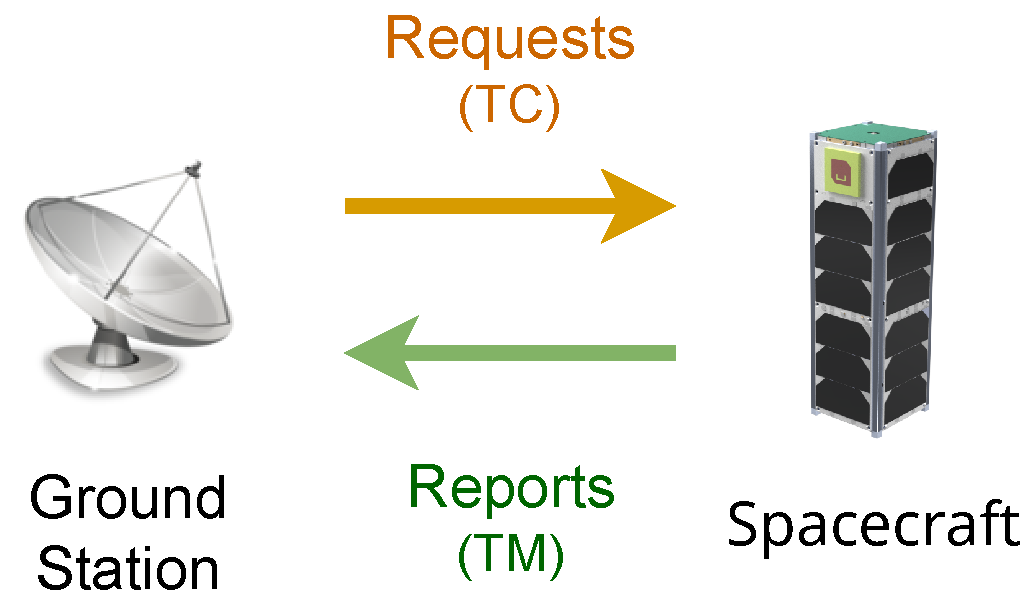
\includegraphics{ECSS-rq}
	\caption{The \ac{PUS} data transfer model}
	\label{fig:pusmodel}
\end{marginfigure}

\subsection{The \acs{ECSS} services}

This standard is intended for use in any space mission, complementing other standards for mission-specific operations, communications or file transfer. Its authors recommend \acs{PUS} users to tailor it to their needs, viewing it as a ``menu'' from where the applicable parts are selected for each specific mission. In summary, the following 20 distinct ``services'' are provided in the standard \autocite{ECSS-E-ST-70-41C,ECSS-E-70-41A,kaufeler_esa_standard_1994}:

\marginnote[1cm]{%
	\textbf{Application Process}: Any physical (hardware) or logical (software) entity that can receive telecommands and generate telemetry in terms of the \acs{PUS}
	
	\textbf{Event}: Occurence of a set of conditions that can arise during the mission, such as:
	\begin{compactitem}
		\item Autonomous actions taken
		\item Detected fault or anomaly
		\item Predefined steps of a process
	\end{compactitem}
	
	\textbf{Parameter}: Readable and modifiable data container that can represent:
	\begin{itemize}
		\item Basic system or component settings
		\item Sensor measurements and other telemetry values
		\item \acs{FDIR} results and diagnostics
	\end{itemize}
}


\begin{compactitem}
	\item \textbf{\texttt{ST[01]}: Request verification}
	
	Provides acknowledgement or failure reports for executed commands. This service essentially informs the operators about the status of \ac{TC} sent to the spacecraft, and reports any occurred errors during parsing or execution.
	
	\item \textbf{\texttt{ST[02]}: Device access}
	
	Allows toggling, controlling and reconfiguring any on-board peripherals that do not support the \ac{PUS} paradigm, but rely on simpler protocols to communicate.
	
	\item \textbf{\texttt{ST[03]}: Housekeeping}
	
	Produces periodic reports containing values of on-board parameters. This service essentially composes the periodic \acs{RF} \textbf{beacon} of the satellite, by storing and transmitting parameter values without any prior \acs{TC} request.
	
	\item \textbf{\texttt{ST[04]}: Parameter statistics reporting}
	
	Allows reporting statistics (min, max, mean, standard deviation) for specific parameters over specified intervals. This is a memory-efficient alternative to the \texttt{ST[03]} housekeeping service.
	
	\item \textbf{\texttt{ST[05]}: Event reporting}
	
	Generates reports when notable occurrences take place on-board, such as:
	\begin{compactitem}
		\item Autonomous on-board actions
		\item Detected failures or anomalies
		\item Predefined steps during an operation
	\end{compactitem}
	
	\item \textbf{\texttt{ST[06]}: Memory management}
	
	Allows writing and reading directly from an on-board memory unit. This can be useful for debugging and investigative purposes, fetching mission data, or uploading new software to the spacecraft avionics. The service also provides for downlinking and uplinking files in a file system.
	
	\item \textbf{\texttt{ST[07]}: Task management} \emph{(deprecated)}
	
	Allows stopping, suspending or resuming software tasks in case of a contingency. This service has been removed from the standard and is only mentioned as a reference.
	
	\item \textbf{\texttt{ST[08]}: Function management}
	
	Provides the capability of running predefined actions that can receive further parameters. These actions can correspond to payload, platform, or any other functionality.
	
	\pagebreak[4] % to not break the next service in half
	\item \textbf{\texttt{ST[09]}: Time management}
	
	Allows periodic reporting of the current absolute spacecraft time for observability and correlation purposes.
	
	\item \textbf{\texttt{ST[10]}: Time packet} \emph{(deprecated)}
	
	Used in the past for time packet generation. This service has been removed from the standard and is only mentioned as a reference.
	
	\item \textbf{\texttt{ST[11]}: Time-based scheduling}
	
	Allows the operators to \textbf{``time-tag''} telecommands for execution at future timestamps, instead of immediately.
	
	\item \textbf{\texttt{ST[12]}: On-board monitoring}
	
	This service allows checking parameter values to ensure that they remain within configurable limits. Whenever a violation occurs, an \texttt{ST[05]} event can be optionally generated for further processing.
	
	\item \textbf{\texttt{ST[13]}: Large packet transfer}
	
	Provides a method of message segmentation, for message payloads that are too large to fit within the maximum allowed length for \ac{TC} or \ac{TM}.
	
	\item \textbf{\texttt{ST[14]}: Real-time forwarding control}
	
	This service is responsible of controlling which types of generated reports are immediately transmitted to the \acl{GS}.
	
	\item \textbf{\texttt{ST[15]}: On-board storage and retrieval}
	
	This service allows storing generated reports on-board, as well as their commanded mass retrieval when the spacecraft has \acl{GS} visibility.
	
	\item \textbf{\texttt{ST[16]}: On-board traffic management} \emph{(deprecated)}
	
	Allows monitoring the status and load of an on-board data bus and provides commands for resolution of errors. This service has been removed from the standard and is only mentioned as a reference.
	
	\item \textbf{\texttt{ST[17]}: Test}
	
	This service allows performing on-board connection and ``are-you-alive'' checks.
	
	\item \textbf{\texttt{ST[18]}: On-board operations procedure}
	
	Allows loading, controlling (start, suspend, resume, abort) and configuring On-Board Control Procedures, which are sequences of commands written in an application-specific language.
	
	\item \textbf{\texttt{ST[19]}: Event-action}
	
	Provides the operators with the capability of autonomously executing \acp{TC} when an \texttt{ST[05]} event is triggered.
	
	\item \textbf{\texttt{ST[20]}: On-board parameter management}
	
	Provides the capability of reading and setting on-board parameters. Parameters are some of the most important entities defined in the \acs{PUS}, and can represent:
	\begin{itemize}
		\item Read-write configuration variables for the system or lower-level components
		\item Read-only sensor and other telemetry values
		\item \ac{FDIR} results and diagnostics
	\end{itemize}
	
	\item \textbf{\texttt{ST[21]}: Request sequencing}
	
	Allows operators to load series of \acp{TC} to be executed in a sequential order.
	
	\item \textbf{\texttt{ST[22]}: Position-based scheduling}
	
	Provides the capability of executing \acp{TC} when the spacecraft reaches a specific point in its orbit.
	
	\item \textbf{\texttt{ST[23]}: File management}
	
	Provides the capability of managing on-board file systems, with functions such as \emph{copy}, \emph{move}, \emph{delete}, or \emph{create directory}.
\end{compactitem}

\section{The SAVOIR standard}
The \texttt{SAVOIR-HB-003} handbook describes in detail the processes and \acs{FDIR} methodology, based on results \& lessons learned from previous space missions. In this chapter, we will provide brief commentary on the parts concerning a low-cost CubeSat mission.

\subsection{\acs{FDIR} process steps}
\bgroup
\Crefname{enumi}{Step}{Steps}

The steps of the \acs{FDIR} process are defined as follows:
\begin{enumerate}
	\setcounter{enumi}{-1}
	\item \textbf{Requirement specification}: Here, based on the needs of each mission, we analyse the requirements of the system for reliability \& availability, and extract the relevant technical \acs{FDIR} requirements, in functional and performance terms. In this stage, no solutions or design decisions are taken, but we define the problems that must be solved and the relevant success criteria.
	\label{itm:fdir_reqs}

	
	Although the formulation of technical specifications for random events and failures is difficult, especially if there is a lack of reliability data, the handbook suggests a set of technical specifications \autocite[42]{SAVOIR-HB-003} that can be used by missions. A large set of these specifications are also met by the design presented in the following chapters.
	
	\item \textbf{Concept definition}: This stage involves the comparison of the general \acs{FDIR} strategies that can solve the requirements of \Cref{itm:fdir_reqs}. Solutions include redundancy, cross-strapping, \acl{TMR} or inherently reliable (high-cost) components.
	
	
	\label{itm:fdir_concept}

	\item \textbf{Architecture}: This step defines the \acs{FDIR} design on a general level based on the system's capabilities, without implementation details, but with enough information for the system structure and the interfaces between elements.
	
	\item \textbf{Detailed design}: Before completing the full design of the \acs{FDIR}, we have to prepare the \textbf{\acf{FMEA}} \autocite{carlson_effective_fmeas_2012} for the system and its subsystems. The \acs{FMEA} is the \textbf{list of all possible failure modes} for satellite elements, where the severity and compensating provisions of each are listed in a standard way.
	
	\label{itm:fdir_cdr}
	
	
	Then, for every feared event of the \acs{FMEA} catalogue, we perform the \textbf{\acf{HSIA}} \autocite{ECSS-Q-ST-30-02C}. In essence, this is where the \textbf{observed data} and \textbf{recovery \& isolation actions} are listed for each failure.
	
	Apart from the aforementioned, the exact operating method and flow of the \acs{FDIR} is detailed for every satellite mode, with special attention given to \emph{Safe Mode} (\Cpageref{itm:safe_mode}).
	
	\item \textbf{Implementation \& Verificaton}: At this stage, the \acs{FDIR} hardware and software are constructed, ready to detect and respond to satellite failures. Additionally, for every item in the \acs{HSIA}, \textbf{verification} is performed by analysis or testing. In particular, each feared event must be simulated, and the correct handling of it by the system must by ensured.
	\label{itm:fdir_valid}
	
	\item \textbf{Validation}: In this stage we perform \textbf{system-level} tests of the \acs{FDIR} after assembly \& integration of the entire spacecraft, as part of the test campaign.\footnote{May contain functional system tests (ambient tests) or environmental tests}
	
	\item \textbf{In-operations preparation}: In the last step, final changes are made to the literature \& documentation to enhance the remote operability of the mission.
\end{enumerate}


Although all the above steps have high significance, ``lean'' missions need to especially focus on requirements (\Cref{itm:fdir_reqs}), concept definition (\Cref{itm:fdir_concept}), detailed design (\Cref{itm:fdir_cdr}) and verification (\Cref{itm:fdir_valid}). A simple example of an application of this process can be found in \Cref{cap:practical}.

At this point, it should be made clear that the \acs{FDIR} design process and the system reliability analysis in general should be taken into account \textbf{throughout the lifetime} of a space project, and not only after the rest of the platform has been designed or implemented. The \ac{RAMS} domain is directly linked to all other subsystems, receiving the required inputs but also heavily influencing the rest of the design. In particular, young CubeSat projects tend to not pay the necessary attention to the reliability domain \autocite{langer_reliability_estimation_2017}.

\egroup
\subsection{Proposed architecture}

The handbook proposes some principles for the architectural design of an \acs{FDIR} system, the first of which considers it as a \textbf{hierarchical} system, where minor failures are caused and corrected at component level, or are propagated as major failures to the rest of the system and require more impactful recovery actions.

\begin{figure}
	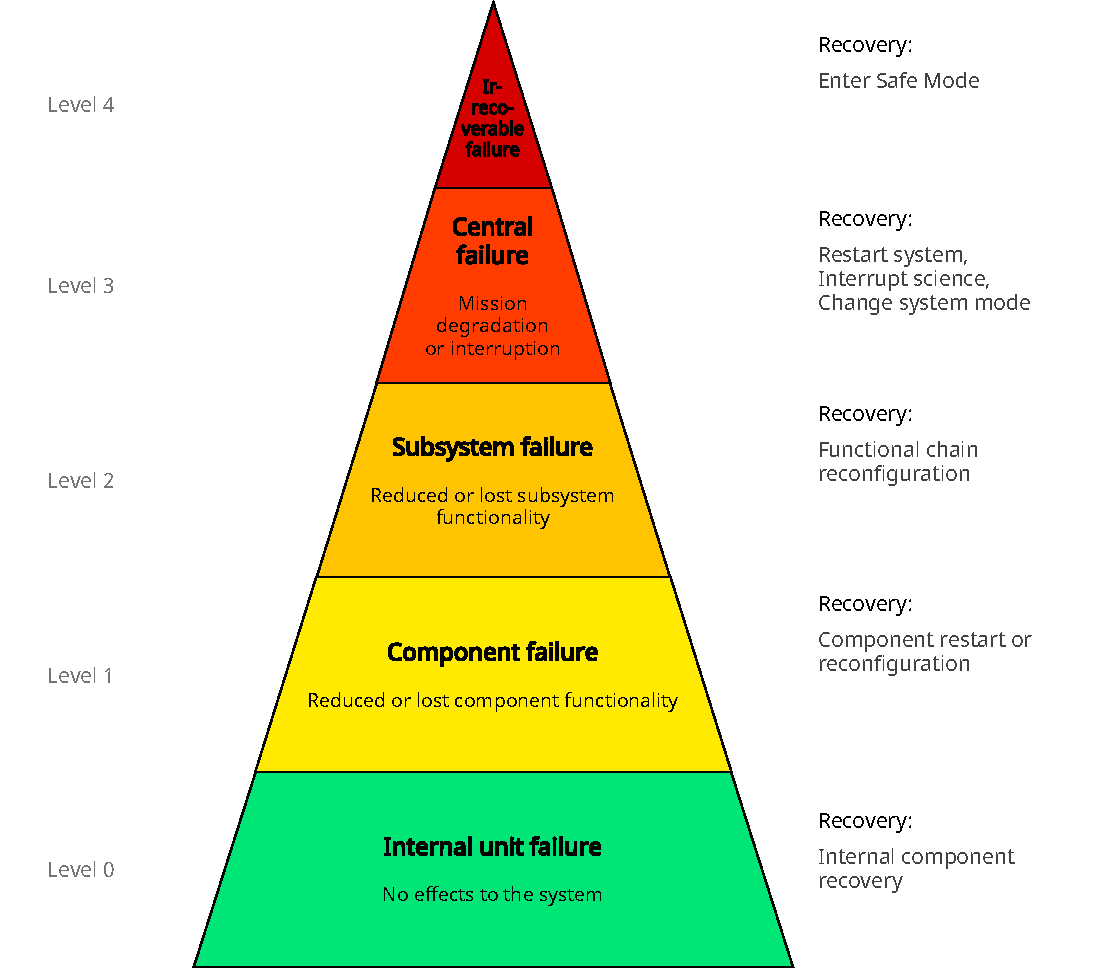
\includegraphics{FDIR-levels-en}
	\caption[Suggested FDIR levels hierarchy]{Suggested FDIR levels hierarchy. Each mission can choose a different set of levels to simplify or refine the implementation.}
	\label{fig:FDIR-levels}
\end{figure}

Moving on, a \textbf{configurable} implementation is proposed that takes advantage of the spacecraft's \textbf{database} in order to store the detection and recovery events. The database and communication tools from the \textbf{\acs{PUS} services} of \Cref{sec:pus} are utilised to fully meet these requirements. This logic entails the following:
\begin{compactenum}
	\item Reliability-related data are stored in \textbf{parameters} (e.g.\ sensor values, peripheral status)
	\item These parameters are \textbf{monitored} by the \emph{on-board monitoring} service. When a parameter gets out of bounds, a failure event is assumed.
	\item Each out-of-bounds parameter creates an \textbf{event} that is telemetered to the ground segment.
	\item Each event is associated with an \textbf{action}, stored in the \emph{event-action} service.
	\item This action may contain one or more procedures to correct the failure.
\end{compactenum}

\begin{figure*}[h]
	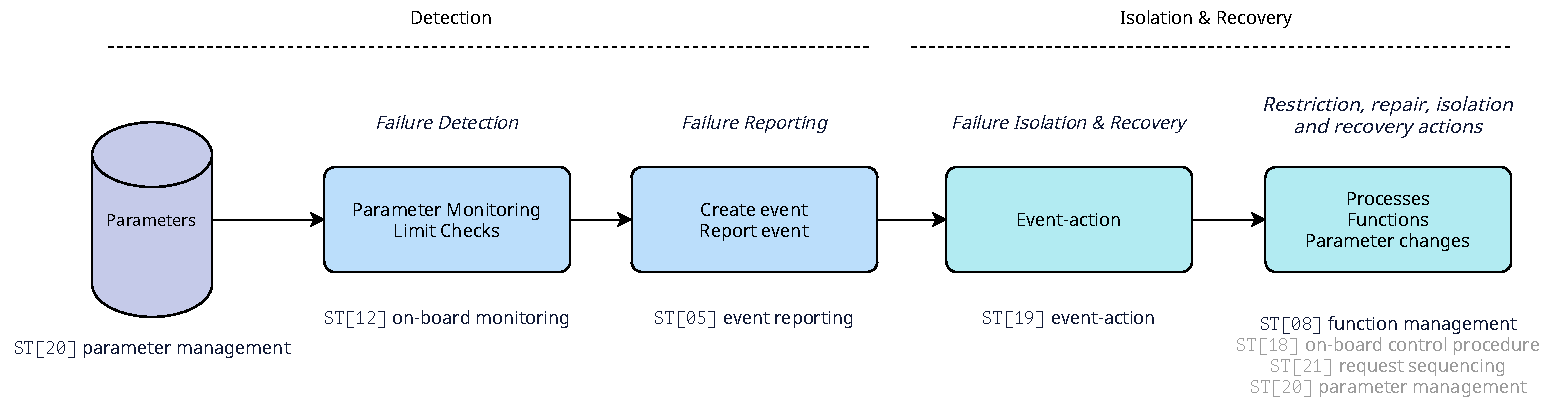
\includegraphics{FDIRpus-en}
	\caption{Data flow for failure detection}
	\label{fig:fdirpus}
\end{figure*}

The above logic is summarized in \Cref{fig:fdirpus}. Its importance lies in that it provides a \textbf{structured} way for the system to handle any of the predicted problems, but at the same time enables developers and operators to:
\begin{compactitem}
	\item Obtain all information on the operational status of components and sensor values.
	\item Safely interfere with the complete operation of the \acs{FDIR} without changing the source code.
	\item Partially or completely disable \acs{FDIR}, if necessary for diagnostic purposes.
	\item Use a ready and tested \acs{ECSS} services software suite to implement all of the above, reducing cost and development time.
	\item Avoid unconfigurable ``hard-coding'' of \acs{FDIR} procedures at various points in the code.
\end{compactitem}

\chapter{\acs{FDIR} in AcubeSAT}
\label{cap:acufdir}

In this chapter, a case study of the application of the above (\Cref{cap:savoir}) is performed, targetting the AcubeSAT mission (\Cref{cap:acubesat}). More specifically, we have analysed the design decisions taken, the implemented parts of the standards, and the specific actions that depend on the mission and experimental profiles of AcubeSAT \autocite{FMEA}.


\section{Basic principles}
\label{sec:fdirbaspri}

AcubeSAT's \acs{FDIR} needs mostly stem from the mission requirements (\Cref{sec:su_fdir}) and the technical capabilities of a low-cost system (\Cref{cap:acubesat}). More specifically, the basic principles are:
\begin{enumerate}
	\item \textbf{Modularity:} \acs{FDIR} should not be hard-coded in software, but should allow for easy modifications based on a well-structured database.
		\item \textbf{Autonomy:} The satellite should be able to survive in orbit for more than \SI{24}{} hours without communication with the \acs{GS}, and should be able to remain in any system mode, especially \emph{Science Mode}.
		\item \textbf{Configurability}: It is very difficult to predict the correct thresholds and behaviour of the \acs{FDIR} system and all components in orbit. Therefore, the operators should be given the possibility to fully configure and tune the \acs{FDIR} if necessary. This configurability may include disabling checks, modifying erroneous limits, or even adding new monitoring definitions.
		\item \textbf{Observability,} by offering a large amount of information to the ground station in order to diagnose problems.
		\item \textbf{No assumptions} for correct equipment functionality. Any software error condition or invalid input should be considered possible.
		\item \textbf{Availability:} AcubeSAT benefits from long operational times in orbit, since this allows downloading larger amounts of scientific data and observability-related telemetry. In addition, brief interruption of any subexperiment may inherently lead to its complete failure (\Cref{sec:su}). Therefore, AcubeSAT follows a \emph{fail-operational} rather than \emph{fail-safe} approach on non-critical aspects.
		\item \textbf{Design} based on reliability. The team tries to implement design changes, to the extent possible by a low-cost CubeSat mission, before actual development or verification of the system.
	\end{enumerate}
	
The above principles are covered by \acs{SAVOIR}'s logic (\Cref{cap:savoir}), which is also implemented in AcubeSAT.

The levels of \acs{FDIR} in AcubeSAT are the following three:
\begin{enumerate}[label=Level \arabic*]
	\item \textbf{Unit}/\textbf{Component}: Here, failures at component-level (e.g.\ temperature sensor) are detected and corrected. Simple failures at this level do not affect the next one, and can typically be corrected by simple actions (e.g.\ component power-cycle).
	
	This level is typically handled by the microcontroller of each subsystem. Although failures here may not be detected by other subsystems, the corresponding telemetry must be produced to provide to ensure observability from ground, or to predict other failures not detected autonomously.
	\item \textbf{Subsystem}: This includes serious failures affecting the entire operation of a subsystem (e.g.\ overheating, no response to pings, etc). These failures do not necessarily halt the satellite's operations, but can be corrected by reboots or changes to the subsystem settings.
	
	Failures at subsystem level and above are handled by the \acf{OBC} microcontroller, which contains the software to detect and recover from them. However, in the event of a failure of the \acs{OBC}, the \ac{ADCS} takes over the responsibility of the \acs{FDIR}.
	\item \textbf{System}: This includes failures which cannot be corrected au\-to\-nom\-ous\-ly by the system (e.g.\ insufficient power, excessive angular velocity). The recovery action for system-level failures is usually to enter \emph{Safe Mode}, where only the most basic and vital satellite operations are performed until the failure is repaired by \acl{GS} commands.
\end{enumerate}

\section{Reliable Architectures}
\label{sec:theoretical}

Before implementing the \acs{FDIR}, it makes sense to study the different architectural decisions that can be made during the design of a small satellite system. In particular, the following designs will be compared \autocite{birolini_reliability_engineering_2004}:

\begin{enumerate}
	\item \textbf{Single Component}
	\item \textbf{Double Redundancy}, where two identical components perform the same function, and one can replace the other. This connectivity can follow the logic of \textbf{cold redundancy} or \textbf{hot redundancy}.
	
	In \textbf{cold redundancy}, only one of the components operates at a time, and an external circuit\footnote{or the components themselves, in the case of warm redundancy \autocite[20]{SAVOIR-HB-003}} checks which of the two is not in a fault state, so that control can be handed over to it.

	In \textbf{hot redundancy}, both components are simultaneously functional, performing the same processes, and one component can take over the functional responsibilities of the other in the event of a failure.

	\item \textbf{\acf{TMR}} with voting, where three components are performing the same computations continuously, and a voting circuit selects the output that has the majority amongst the three. Also known as \emph{majority logic}.
\end{enumerate}

Two types of failures will be applied to the aforementioned systems:

\begin{marginfigure}
\centering
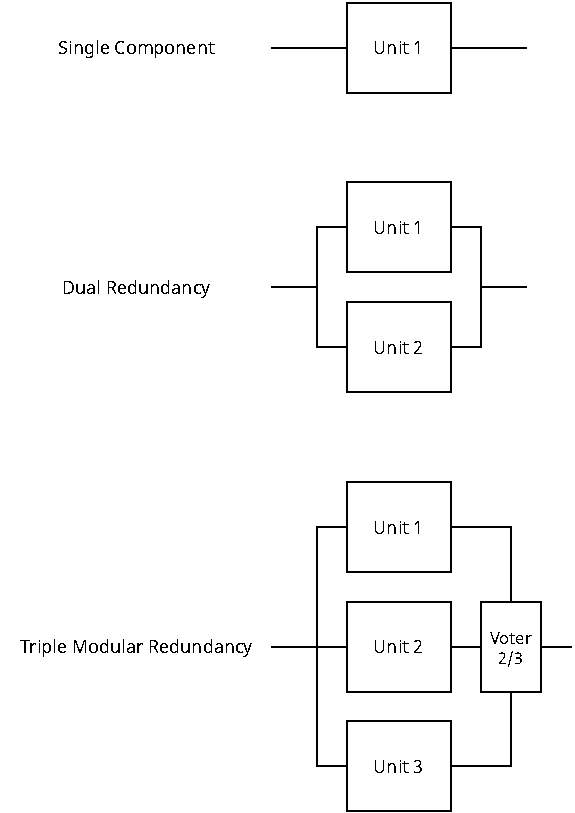
\includegraphics{RedunSchemes}
\caption{Visual illustration of the different considered architectures}
\acusepage{voter}
\end{marginfigure}
\begin{itemize}
\item In \textbf{permanent failures}, we consider events (e.g.\ radiation, loss of memory) that cannot be corrected and result in loss of mission. The analysis here is based on the concept of \e{reliability} \( R(t) \), i.e.\ the probability that the system will survive within a period of time \( t \).
\item In \textbf{temporary failures} we consider events (e.g.\ bit changes, software bugs, message transfer errors) that are transient and usually affect only one measurement, action or result. The analysis here revolves around the concept of the failure rate \( \lambda \), i.e.\ the occurrence frequency of failures in time.
\end{itemize}

As there are no large-scale data available for component failures in the space industry \autocite{esatec-qqd_effective_reliability_2016}, this analysis will present results over a range of reliability values.

As an example, failure rate of a device or unit due to radiation can range between \(10^{-11}\) to \(10^{-1}\) \(\frac{\text{failures}}{\text{second}}\), depending on the radiation environment, the severity of the failure, and the internals of each device \autocite[158-159]{gupta_analysis_single_2017}.

% !!! Code for analysis.

\subsection{Permanent failures (reliability analysis)}

\paragraph{\textbf{Ideal voter}}\hspace{0pt}
\acusepage{voter}


Assuming that the reliability of a component is \(R\), the reliability of \emph{two components} connected in parallel is \autocite[31]{birolini_reliability_engineering_2004}:
\begin{equation}
R_2 = 2R - R^2 = 1 - (1 - R)^2 \label{eq:dual_redun}
\end{equation}
	
\marginnote{In all analyses, we assume that the redundant components are identical and have the same reliability characteristics.}
	
\eqref{eq:dual_redun} applies to \textbf{warm and hot redundancy}, as we assume that the system can recover from permanent failures by moving control to the unaffected component.

On the other hand, most \textbf{cold redundancy} architectures assume that the unused component is inactive or not powered, and therefore is not affected by some failure causes (e.g.\ \acsp{SEL}). Assuming that a component is completely powered off if not active, let:
\begin{align*}
T: & \text{ the time of failure of the 2-component system}\\
T_1: & \text{ the time of failure of the 1\textsuperscript{st} component}\\
T_2: & \text{ the time of failure of the 2\textsuperscript{nd} component, so that } T_1 + T_2 = T
\end{align*}

Then, the conditional probability of failure of the system, given the time of failure of the 1\textsuperscript{st} component, is:
\marginnote[2.5ex]{For some \(t,t_1 \geq 0 \)}
\marginnote[6ex]{From the definition of reliability, \( R(t) = Pr(T>t) \).}
\begin{align*}
Pr\left( T > t \;\middle|\; T_1 = t_1 \right) &= Pr\left( T_1+T_2 > t \;\middle|\; T_1 = t_1  \right) \\
&= Pr\left( T_2 > t - t_1 \;\middle|\; T_1 = t_1  \right) \\
&= Pr\left(T_2 > t - t_1\right) \\
&= R\left(t - t_1\right) \numberthis \label{eq:conditional}
\end{align*}

By the chain rule for probability, we can calculate the unconditional probability of system failure:
\begin{equation}
Pr(T>t) = \lim_{\Delta t \to 0} \sum_{\substack{t_1=0,\\\Delta t,\;2\Delta t,\\\dots}}^{\infty}
Pr\left(T>t \;\middle|\; T_1\in(t_1,t_1+\Delta t) \right) \cdot Pr\left(T_1 \in (t_1,t_1+\Delta t)\right)
\label{eq:prsum}
\end{equation}

\eqref{eq:prsum} uses a limit to work around the restriction imposed by the zero probability \( Pr(T_1 = t_1)\), which should be instead expressed instead of the probability density function \( f(t) \), so that:
\begin{equation}
R(t) = Pr(T > t) = \int_t^\infty f(\tau) \dd{\tau} \label{eq:pdf}
\end{equation}

Using \eqref{eq:pdf}, \eqref{eq:prsum} can be rewritten as a Riemann integral:
\begin{align}
Pr(T>t) &= \int_{0}^{\infty} Pr\left(T>t \;\middle|\; T_1= t_1 \right) \cdot f(t_1) \dd{t_1}
\end{align}
and, after applying \eqref{eq:conditional}:
\begin{align}
Pr(T>t) &= \int_{0}^{\infty} R(t-t_1) f(t_1) \dd{t_1} \label{eq:unfinishedint}
\end{align}

\eqref{eq:unfinishedint} cannot be further processed, since it depends on the exact form of the \(R\) reliability function.

\begin{marginfigure}%
	\centering
	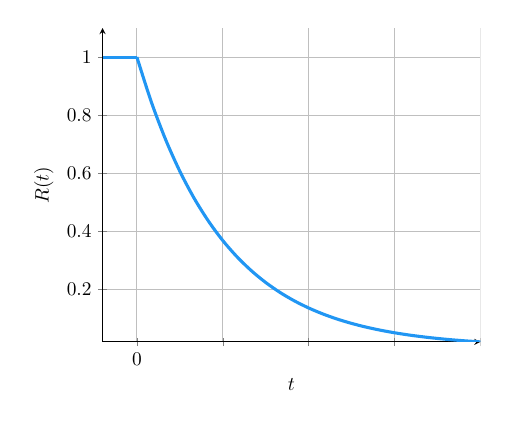
\begin{tikzpicture}[scale=.7]
	\begin{axis}[
	axis lines = left,
	xlabel = \(t\),
	ylabel = \(R(t)\),
	ymajorgrids=true,
	xmajorgrids=true,
	xminorgrids=true,
	ymax=1.1,
	xticklabels={,$0$},
	]
	\addplot[domain=-0.2:0.001, MaterialBlue500, ultra thick] {1};
	\addplot[domain=0:2, MaterialBlue500, ultra thick,smooth] {exp(-2*x)};
	\end{axis}
	\end{tikzpicture}
	\caption{The reliability function of \eqref{eq:typicalR}}
\end{marginfigure}%
In order to provide some indicative results, we will assume a typical reliability function for all components:
\begin{equation}
R(t) = \begin{cases} e^{-at} &\text{ for } t \geq 0 \\ 1 & \text{ for } t < 0 \end{cases} \qquad \text{where } a>0 \label{eq:typicalR}
\end{equation}
with the associated probability density function:
\begin{equation}
f(t) = \dv{R(t)}{t} = ae^{-at} \label{eq:typicalf}
\end{equation}

Then, \eqref{eq:unfinishedint} can be solved further:
\marginnote[14.5ex]{From \eqref{eq:pdf}} %TODO: Check OK distance
\begin{align*}
Pr(T>t) &= \int_{0}^{t} R(t-t_1) f(t_1) \dd{t_1} + \int_{t}^{\infty} R(t-t_1) f(t_1) \dd{t_1}
\\ &= \int_0^t e^{-a(t-t_1)} \cdot ae^{-at_1} \dd{t_1} + \int_{t}^{\infty} f(t_1) \dd{t_1}
\\ &= \int_0^t ae^{-at} \dd{t_1} + R(t)
\\ &= ate^{-at} + R(t)
\\ &= -\ln \left(R(t)\right) \cdot R(t) + R(t)
\\ &= R(t) \cdot (1 - \ln R(t)). \numberthis \label{eq:colddrper}
\end{align*}

 
\newthought{The reliability of} the \emph{\ac{TMR}} system depends on the implementation of the voter. We will distinguish 2 types of voters:
\begin{enumerate}
	\item \textbf{Naive voter}, where a permanent failure in any \emph{two} out of the three components leads to loss of the system.
	
	The reliability of the naive system is \autocite[31]{birolini_reliability_engineering_2004}:
	\begin{align}
	R_3 &= \sum_{i=k}^{n} \binom{n}{i} R^i (1-R)^{n-i}\nonumber\\
	&= \sum_{i=2}^{3} \binom{3}{i} R^i (1-R)^{3-i} \nonumber\\
	&= \binom{3}{2} R^2 (1-R) + \binom{3}{3} R^3 (1-R)^0 \nonumber\\
	&= 3R^2 - 3R^3 + R^3 \nonumber\\
	&= 3R^2 - 2R^3
	\label{eq:tmr}
	\end{align}
	
	\item \textbf{Complex voter}, where if two components fail, the voter can switch to the remaining one, via telecommand or autonomously. This logic is rarely possible to implement, especially if mission-critical components are protected. Additionally, the increased voter complexity inherently reduces its reliability.
	
	For completeness purposes, we cite the reliability of the complex \acs{TMR} system, which stems from the probability that all 3 components fail within \( t \):
	\begin{align}
	R_{3c} &= 1 - (1 - R)^3
	\label{eq:tmr_complex}
	\end{align}
\end{enumerate}


\begin{figure}
	\centering
	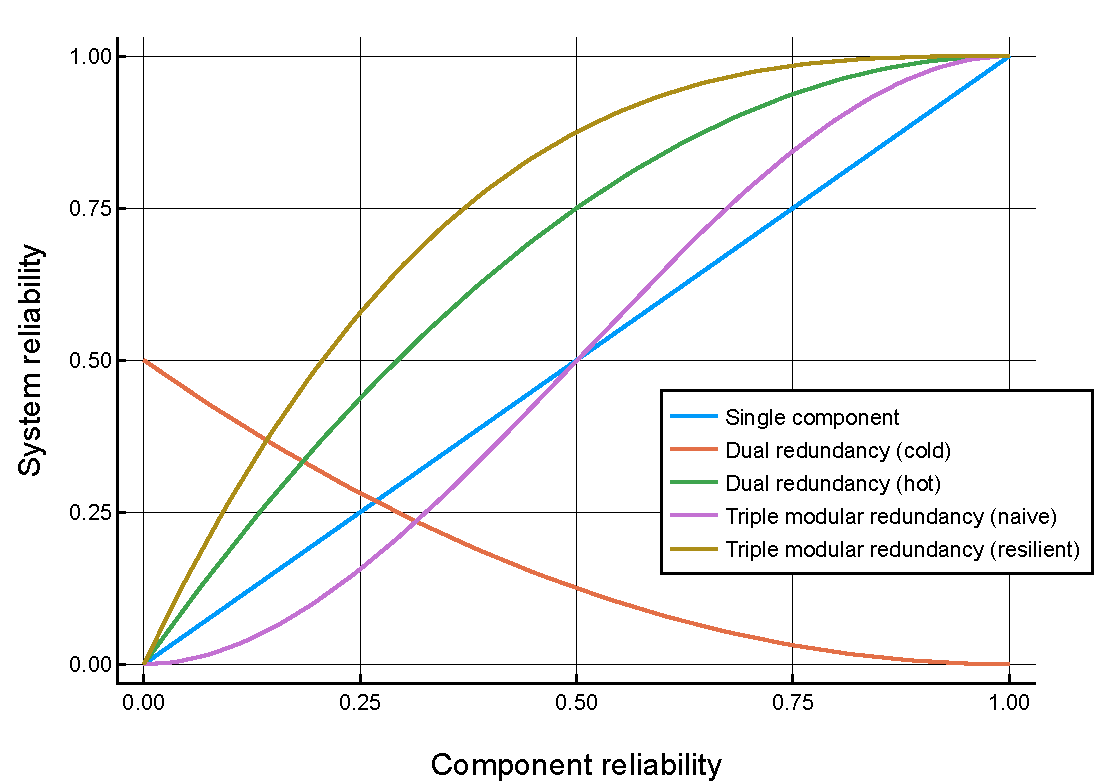
\includegraphics{analysis/reliability_norepair_en}
	\caption[Resilience of a compound system to permanent failures (assuming an ideal voter)]{Resilience of a compound system to permanent failures (assuming an ideal voter --- higher \(R\) is better)}
	\label{fig:reliability_norepair}
\end{figure}

The results of \eqref{eq:dual_redun}, \eqref{eq:colddrper}, \eqref{eq:tmr} and \eqref{eq:tmr_complex} are shown in \Cref{fig:reliability_norepair}. It can be observed that, compared to the single component, the use of two redundant components increases the reliability of the system to a certain extent, since failures of one component can be repaired, but failures in both are catastrophic. In contrast, \textbf{naive \acs{TMR} introduces more points of failure}. Since failure of any combination of 2 of the 3 components is catastrophic, majority logic is sometimes less reliable than dual redundancy.

\paragraph{\textbf{Vulnerable Voter}}\hspace{0pt}
\acusepage{voter}

The study of a vulnerable voter circuit in \acs{TMR} is of particular interest. In the context of this analysis, we will consider the independent reliabiliy value \( R_v < 1 \) of the voter. From \autocite[31]{birolini_reliability_engineering_2004}, we have:
\begin{align}
R_{3+v} &= (3R^2 - 2R^3)R_v \nonumber \\
&= R_3R_v
\end{align}
and the reliability of the compound system is simply multiplied with the voter's reliability. The voter reduced the \acs{TMR} system reliability in a linear fashion.

\begin{figure}
	\centering
	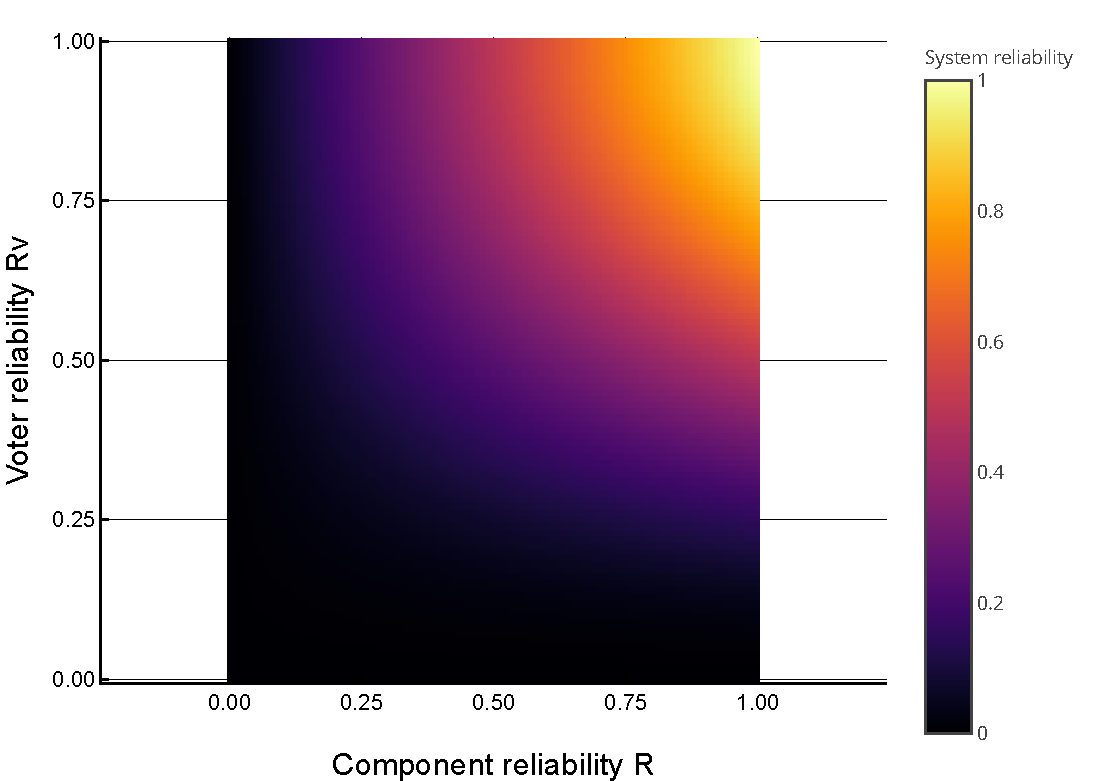
\includegraphics{analysis/reliability_norepair_voter_en}
	\caption[Resilience of the TMR system to permanent failures (assuming a vulnerable voter)]{Resilience of the \acs{TMR} system to permanent failures (assuming a vulnerable voter --- higher \(R\) is better)}
	\label{fig:reliability_norepair_voter}
\end{figure}

\subsection{Temporary failures (failure rate analysis)}

If \( \lambda \) is the failure rate of one component, the failure rate of a cold-redundant system is equivalent to \( \lambda \), since only one component is active at a time, and the deactivated one cannot fail.

\marginnote{We assume that component failures are independent events.}

In the case of hot redundancy, both components may fail, at a rate of \( \lambda \) each. We assume that component failures follow a Poisson distribution \autocite[35]{birolini_reliability_engineering_2004}. Then, the probability that \(k\) failures occur in a time interval is given by \autocite[60]{yates_probability_stochastic_2014}:
	\begin{equation}
	P(X=k) = \frac{\lambda^ke^{-\lambda}}{k!}
	\end{equation}
	
\marginnote{It is interesting to locate the failure rate where the probability of 2 failures is equal to 1\% of the probability of 1 failure, i.e. \(P(X=2) = 0.01P(X=1) \implies \frac{\lambda^2e^{-\lambda}}{2} = 0.01 \lambda e^{-\lambda } \implies \lambda = 0.02 \). So for \( \lambda < \SI{2e-2}{} \) the hypothesis is valid.}

To simplify the analysis, we will assume that only \(k = 1\) failure can occur in the time interval defined by the parameter \( \lambda \). This assumption is safe, as we can study short time intervals (usually seconds), where it is extremely unusual for more than 1 failure to occur.
	\begin{equation}
	P = P(X) = \lambda e^{-\lambda}
	\end{equation}
	
In hot dual redundancy, it is not always possible to identify the wrong and correct output, so a failure in either component is considered a system failure. Thus, if \(X_1\) and \(X_2\) are the failure events of the 1\textsuperscript{st} and 2\textsuperscript{nd} component respectively:
\begin{align}
P_2 = P(X_1\text{ or }X_2) &= 1 - (1 - P(X))^2 \nonumber\\
&= 1 - \left(1 - \lambda e^{-\lambda} \right)^2 \nonumber\\
&=  2 \lambda e^{-\lambda} -\lambda^2e^{-2\lambda} \label{eq:lambda}
\end{align}
	
\eqref{eq:lambda} does not follow the Poisson distribution, so it is not easy to directly derive the failure rate of the system. However, we can extract the \emph{average} failure rate, let \( \lambda_2 \), by trying to fit the Poisson distribution to the non-Poisson result:
\begin{align}
\lambda_2e^{-\lambda_2} = P_2 \label{eq:lambert_eqn}
\end{align}
\marginnote{Alternatively, we can ignore the negligible 2\textsuperscript{nd} term of \eqref{eq:lambda}, and have \( P_2 = 2\lambda e^{-\lambda} \). Since \(e^x \approx 1\) very close to \(x=0\), \eqref{eq:lambert_eqn} becomes:
	\[
	\lambda_2 = 2\lambda
	\]
	The above is also confirmed intuitively. After introducing 2 components, the error rate doubled.
}%
		
	\eqref{eq:lambert_eqn} can be solved by using the Lambert W function \autocite{weisstein_lambert_wfunction_2003} defined as follows:
\begin{align}
	\text{for } w,z \in \mathbb R:\quad we^w = z \iff w = W_k(z) \text{ for some } k \in \mathbb Z
\end{align}
		
Subsequently, we can compute \(\lambda_2\):
\begin{align}
	\lambda_2 = -W_k(-P_2)
	\label{eq:l2}
\end{align}


\newthought{In the \acs{TMR} system}, the complete failure event is equivalent to the failure of at least 2 of the components. Therefore, similar to \eqref{eq:tmr}, we have:
\begin{align}
P_3 &= 3P^2 - 2P^3 \nonumber\\
&= 3\left(\lambda e^{-\lambda}\right)^2 - 2\left(\lambda e^{-\lambda}\right)^3
\end{align}
and, following the same methodology as \eqref{eq:l2}:
\begin{align}
\lambda_3 = -W_k(-P_3)
\label{eq:l3}
\end{align}

The above results can be calculated numerically, and are shown in \Cref{fig:reliability_repair}.

\begin{figure}
	\centering
	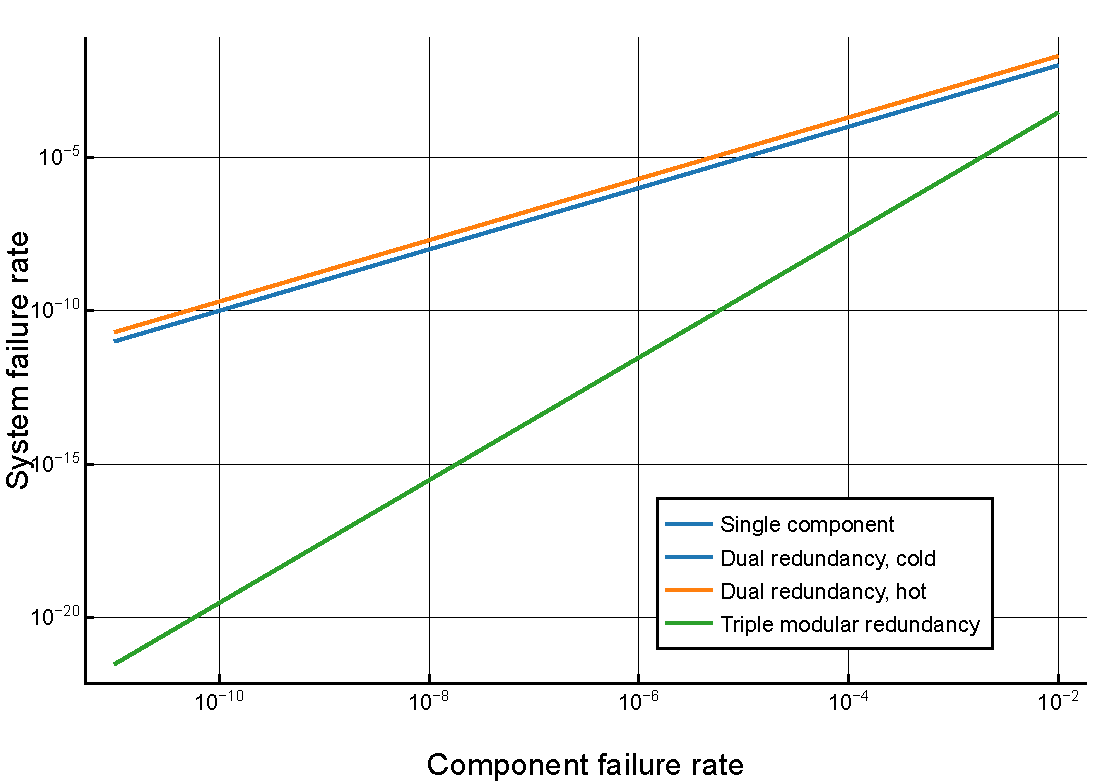
\includegraphics{analysis/reliability_repair_en}
	\caption[Resilience of a compound system to temporary errors]{Resilience of a compound system to temporary errors (assuming an ideal voter --- smaller \(\lambda\) is better)}
		\label{fig:reliability_repair}
	\end{figure}
	
	\subsection{Conclusion}
	
The results of \Cref{fig:reliability_norepair,fig:reliability_repair} are summarised in \Cref{tab:calcuresults}, along with the implementation complexity of each architecture.
	
%	\FloatBarrier
As shown, each solution comes with a different set of positives and negatives. The use of voting can overwhelmingly reduce the failure rate for temporary failures, while the use of pure redundancy improves the behaviour on permanent failures and allows recovery from catastrophic faults.

\begin{table}[h]
	\caption{Summary of reliable architecture analysis}
	\label{tab:calcuresults}
	\begin{adjustbox}{center}
	\begin{tabular}{@{}rlll@{}}
		\toprule
		& \multicolumn{2}{l}{Tolerance to failures} & \\ \cmidrule{2-3}
		Architecture & Permanent & Temporary & Complexity \\ \midrule
		Single component & \color{MaterialGrey800} Normal & \color{MaterialGrey800} Normal & \color{MaterialGreen600} Low \\
		Dual redundancy, cold & \color{MaterialGreenA700} Very good & \color{MaterialGrey800} Normal & \color{MaterialOrange900} Medium\\
		Dual redundancy, hot & \color{MaterialGreen600} Good & \color{MaterialOrange900} Worse & \color{MaterialOrange900} Medium\\
		Triple Mod. Redundancy & \color{MaterialLime800} Better {\footnotesize(if \(R > 0.5\))} & \color{MaterialGreenA700} Excellent & \color{MaterialRed800} High \\ \bottomrule
	\end{tabular}
	\end{adjustbox}
	%\vspace{1ex}
\end{table}



The final choice of architecture depends on the requirements \& needs of each project. For example, in manned missions, it is common to use \acs{TMR} on the flight computer, so that no error can compromise the safety of the passengers.

In the AcubeSAT mission, where vulnerable \acs{COTS} components are used, the emphasis is on \emph{avoidance of catastrophic effects}. Although temporary failures can potentially degrade the experimental results and system availability, they are considered less critical than permanent ones. Especially in CubeSat projects, the \textbf{complexity} of the chosen architecture must also be taken into account, firstly in relation to the available \textbf{resources} and \textbf{time} of implementation, but also because a complex architecture can itself reduce the reliability of the system if not implemented and tested properly.

The typical architecture chosen in AcubeSAT is as follows:
\begin{itemize}
	\item In \textbf{sensor} networks (e.g.\ temperature, pressure, magnetic field), \emph{dual redundancy} is applied, and the possibility of recovering from the loss of a sensor is given.
	\item For components with \textbf{flight heritage} that have proven their functionality in other missions, it is assumed that the \( R \) value is high enough, and no form of redundancy is implemented.
	\item Specifically for microcontrollers, the chosen option is to use a more expensive \textbf{radiation-resistant} \acs{MCU}, with an inherently higher \( R \) (\Cref{sec:obdh}), rather than attempting to increase \( R \) using redundancy.
\end{itemize}

\FloatBarrier
\section{Detailed \acs{FDIR} Actions}

The following section presents a list of the implemented methods to detect, prevent and recover from errors occurring on the satellite. For each possible failure identified in \acs{FMEA} \autocite{retselis_acubesat_fmea_2020}, one or more detection and correction methods are selected from \Cref{tab:fdir_detect,tab:fdir_preventive,tab:fdir_correction}, and tailored to the respective element.


\clearpage
\subsection{Detection Actions}
\begin{table*}[h]
	\centering
	\caption[][10pt]{AcubeSAT \acs{FDIR} failure detection methods}
	\label{tab:fdir_detect}
	\renewcommand{\arraystretch}{1.3}
	\begin{tabularx}{\textwidth}{@{}cL{5cm}X@{}}
		\toprule
		Level & Method & Description \\ \midrule
		Unit & \textbf{Self-test does not return a correct value} & Connected peripherals may have self-test capabilities or may have stored default values that cannot be changed. \\
		Unit & \textbf{Value out of range} & Unexpected sensor values may indicate actually dangerous environmental conditions, or simply faulty (e.g.\ \acs{SEFI}) sensors. Dual or triple redundancy can increase observability in this case. \\
		Unit & \textbf{Sampled sensor values very different} & \\
		Unit & \textbf{No response or incoherent values} & The unit or interface may be faulty. \\
		Unit & \textbf{Abnormally high current consumption} & May be observed in units suffering from short circuits or \acs{SEL}. \\
		Unit & \textbf{Scrubbing error} & Error correction and detection algorithms can indicate bit flips. \\
		Subsystem & \textbf{No response to \acs{CAN} commands} & May be due to failure of the subsystem, or the \acs{CAN} transceiver. \\
		System & \textbf{No \acsp{TC} have been received for some time} & The \acs{GS} sends periodic ``refresh'' commands to the satellite on each pass. Failure to receive means loss of communication. \\
		Software & \textbf{Hardware exception} & May be due to division by 0, attempting to access inaccessible memory, etc. \\
		Software & \textbf{Assertion failed} & Using the C \texttt{assert} function \\
		Software & \textbf{Unexpected microcontroller reset} & Possibly a watchdog trigger \parencite{beningo_review_watchdog_2018} or bug \\
		Software & \textbf{\acs{TMR} variables wrong} & \\ \bottomrule
	\end{tabularx}
\end{table*}

\clearpage
\subsection{Preventive Actions}

\begin{table*}[h]
	\centering
	\caption[][10pt]{AcubeSAT \acs{FDIR} failure prevention methods}
	\label{tab:fdir_preventive}
	\renewcommand{\arraystretch}{1.5}
	\begin{tabularx}{\textwidth}{@{}lcX@{}}
		\toprule
		\# & Level & Action \\ \midrule
		1 & Hardware & Radiation-tolerant microcontroller \\
		2 & Hardware & Microcontroller watchdogs \parencite{beningo_review_watchdog_2010} \\
		3 & Hardware & System-level watchdogs \\
		4 & Hardware & Hardware error correction \& detection algoritmhs \\
		5 & Hardware & Dual redundancy in software memory \\
		6 & Hardware & Current-limiting circuits \\
		7 & Hardware & Subsystem overvoltage and overcurrent protection \\
		8 & Hardware & Use of radiation-resistant \acs{MRAM} memory \\
		9 & Hardware & Dual redundancy in sensors \\
		10 & Hardware & Derating in power electronics \\
		11 & Hardware & Placement of vulnerable components close to the centre of \acsp{PCB} to reduce the effect of radiation dose \\
		12 & Hardware & Selection of components with available radiation test results \\
		13 & Hardware & Dual redundancy on the \acs{CAN} bus \\
		14 & Software & Parity bit in the \acs{CAN} messages \\
		15 & Software & Software error detection \& correction algorithms \\
		16 & Software & Failure and power loss tolerant filesystem \\
		17 & Software & \acs{ADCS} input filtering \\
		18 & Operational & Automatic periodic restarts \\
		19 & Operational & Avoidance of dangerous operations in areas with high radiation levels \\
		20 & Operational & Evaluation of available resources \& budgets before starting a subexperiment \\ \bottomrule
	\end{tabularx}
\end{table*}

\clearpage
\subsection{Corrective actions}

\begin{table*}[h]
	\centering
	\caption[][10pt]{AcubeSAT \acs{FDIR} failure correction methods}
	\label{tab:fdir_correction}
	\renewcommand{\arraystretch}{1.5}
	\begin{tabularx}{\textwidth}{@{}lL{3cm}X@{}}
		\toprule
		Level & Action & Description \\ \midrule
		& \textbf{None} & Many problems are corrected automatically, or there is no way to correct them (and they do not significantly affect the operation of the rest of the satellite). \\
		Unit & \textbf{Restart unit} & This recovery method is associated with temporary faults that may occur in the software or hardware of a device. Such faults may result from bugs that were missed during testing, or from radiation-induced \acsp{SEFI}. \\
		Unit & \textbf{Power-cycle unit} & Some errors cannot be corrected until the power to the affected unit is cut off. Radiation-induced \acsp{SEL} are the main reason for this. \\
		Module & \textbf{Isolate unit} & If a module cannot be repaired, the next step is to ignore its values and/or to disconnect its power supply, so that the rest of the system is not affected by its erroneous outputs. \\
		Subsystem & \textbf{Power-cycle subsystem} & Radiation or other failures can lead a subsystem into an unexpected state, from which it can only escape by restarting. \\
		Subsystem & \textbf{Reconfigure subsystem} & If a permanent failure cannot be corrected by a reboot, the spacecraft should attempt to resume normal operation. This can be done by changing the default configuration of a subsystem, e.g.\ by selecting different sensors, by changing the functionality of the subsystem, or by delegating its tasks to another module. \\
		System & \textbf{Abort current function} & The currently running process (e.g.\ experiment initialisation, \acs{TM} transmission) can be interrupted, as long as this action does not affect the safety of the system. \\
		System & \textbf{Enter safe mode} & This is the last option in the corrective efforts. The satellite enters Safe Mode to prevent further propagation of the fault, when all other actions have failed to resolve the issue. \\ \bottomrule
	\end{tabularx}
\end{table*}

\clearpage
\section{\acs{FDIR} functional flow}
\label{sec:fdir_operating_modes}

This section presents the flows and processes of \acs{FDIR} that are executed in orbit. Although the exact process for each component and subsystem is different, a general hierarchical rule is followed that starts at the lowest level (unit/component), and proceeds to system-level, if the relevant failure has not been resolved.

Once the recovery actions are completed, the responsibility shifts to the operators, who must identify the root cause of the problem, and take the necessary actions, if any, to permanently resolve it.

\begin{figure*}[h]
	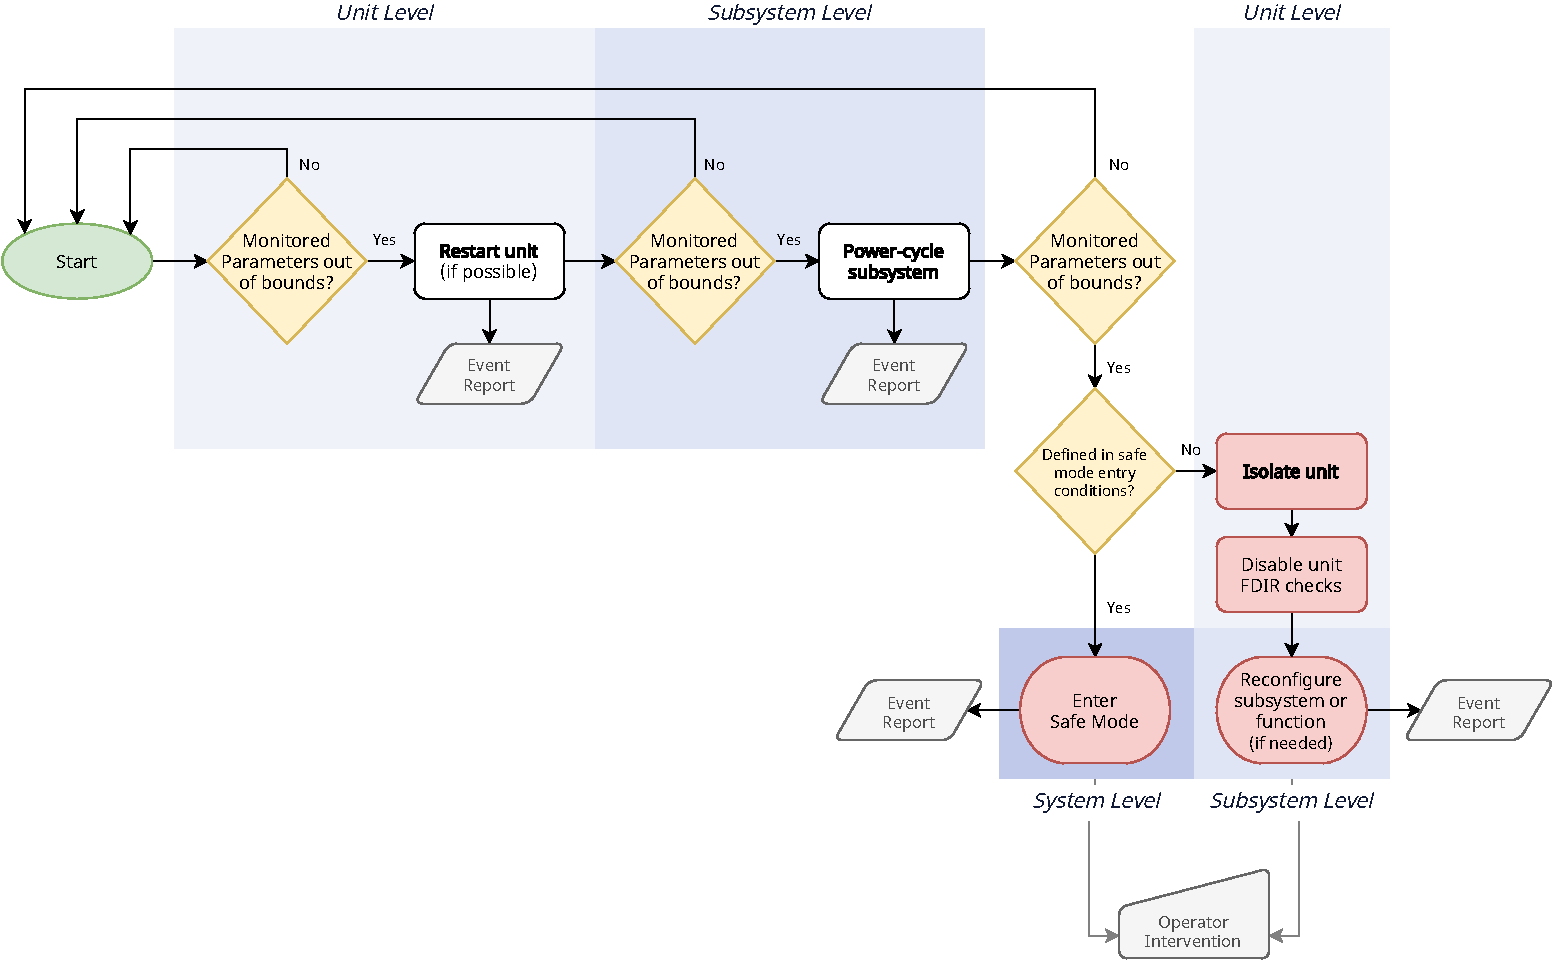
\includegraphics{FDIRgeneric}
	\caption{Generic flow of \acs{FDIR} in all operational modes of the satellite}
	\label{fig:generalflow}
\end{figure*}

The typical flow shown in \Cref{fig:generalflow} describes the usual process of resolving a failure on the satellite. More specifically:
\begin{enumerate}
	\item If an observed parameter is out of bounds, a fix is first attempted at the unit level with \textbf{simple actions} (e.g.\ reset, power-cycle).
	\item If the failure persists, then a subsystem-level resolution is attempted. For critical components, this may mean restarting the entire subsystem; otherwise, it may mean simply powering down the unit.
	
	In technical terms, the separation between the component and subsystem levels is achieved by appropriate usage of the \textbf{\texttt{ST[12]} on-board monitoring service} (\Cref{sec:pus}). Using the \textbf{repetition number} parameter, the operator can set the failure duration thresholds, which are then used to differentiate between the type of recovery actions applied. 	\marginnote[-3ex]{An alternative method of implementation is to define a parameter indicating the state or current step of \acs{FDIR} for each module, and have monitoring definitions triggered according to the value of this parameter.}
	For example, \textbf{2} out-of-limits measurements lead to a sensor \textbf{restart}, while \textbf{5} out-of-limits measurements can lead to complete isolation/\textbf{deactivation}.

	\item If the failure persists but is not critical, the unit and its \acs{FDIR} are permanently disabled, and the subsystem is reconfigured if necessary.
	
	At this point it should be emphasised that the disabled unit should not contribute to any of the satellite's operations. The \texttt{ST[12]} service allows the use of \textbf{check validity conditions}, which can disable a check if it refers to a disabled device or other conditions that prevent it.
	\item If the failure persists, is critical, and there is no other way to correct it, the system enters \textbf{Safe Mode}.
\end{enumerate}

All of the above are executed in the background of each microcontroller as an \acs{RTOS} process. The utilisation of the \acs{PUS} services enables all of the above to be modified in orbit.

\subsection{Safe Mode}
\label{itm:safe_mode}

\begin{figure}[h]
	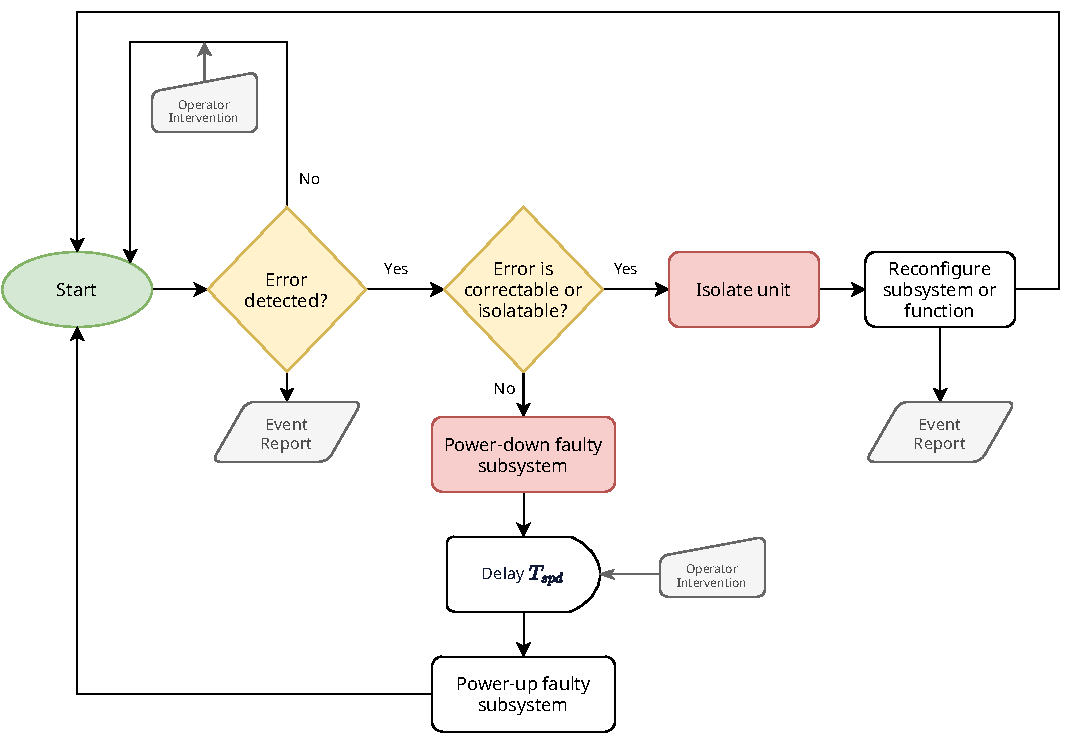
\includegraphics{FDIRsafe}
	\caption{\acs{FDIR} flow in safe mode}
	\label{fig:safeflow}
\end{figure}


The goal of \emph{Safe Mode} is to provide a robust, well-tested and deterministic state where the satellite can operate autonomously, until the operators can remedy the mission-threatening failure. The \acs{FDIR} in Safe Mode also follows the \acs{PUS} principles and AcubeSAT's requirements (\Cref{sec:fdirbaspri}), continuing to allow on-the-fly modifications by operators.

The generic architecture for \acs{FDIR} during Safe Mode is shown in \Cref{fig:safeflow}. Recovery actions include:
\begin{itemize}
	\item Disabling entire \textbf{problematic} subsystems. In the case of \acs{ADCS} and \acs{OBC}, this action is accompanied by significantly reduced spacecraft functionality, but does not prevent control of the spacecraft from the ground. On the other hand, disabling the \acs{COMMS} and \acs{EPS} subsystems prevents any communication between the \acl{GS} and the CubeSat. In any case, the only action that can be taken is to attempt to restart the subsystems after a predetermined time delay, waiting until the satellite reaches more favourable environmental conditions.
	\item Isolating components and reconfiguring subsystems accordingly. The smaller number of active components in Safe Mode translates to a safer design and testing process.
\end{itemize}

AcubeSAT's operators are responsible for determining the cause of the failure and required actions as soon as they receive the telemetry announcing the failure, and must intervene immediately after a safe course of action has been decided. Exit from Safe Mode can \emph{only} be made after \acs{TC}, and only after the initial fault has been corrected and no other faults are evident (e.g.\ due to fault propagation).

The actions that operators can take to recover from failures are:
\begin{compactitem}
	\item Modify the satellite configuration via the \acs{ECSS} services.
	\item More often, change the satellite's \textbf{software}, by uploading updated binary images\footnote{This process requires the re-execution of a full software test campaign on the ground, and a reliable process of reprogramming the satellite in orbit \autocite[45]{DDJF_OBSW}.}
	\item Permanently deactivate all defective units
	\item Wait until the satellite is in favourable environmental (orbital, thermal, solar) conditions
	\item None, if the fault was detected by mistake, or corrected automatically
\end{compactitem}


\section{Next steps}
The combination of \acs{FMEA} and \acs{HSIA} of AcubeSAT contains 928 potential failures, of which 185 are considered critical items \autocite{retselis_acubesat_fmea_2020}.

After formulating the architecture and design of the \acs{FDIR}, its implementation follows. For this purpose, the team is developing a library that implements the \acs{PUS} services\footurl{https://gitlab.com/acubesat/obc/ecss-services} and can meet the needs of this section.

Verification of \acs{FDIR} is the last part of the process, and involves checking for any feared event through hardware or software simulation.

\chapter{Practical demonstration of \ac{FDIR}}
\label{cap:practical}

As a proof of concept for AcubeSAT's \ac{FDIR} implementation, a practical setup to simulate the satellite's behaviour was prepared (\Cref{fig:block}). Key elements of the setup are:
\begin{compactitem}
	\item A Cortex-M7 \textbf{microcontroller}, used to simulate a \textbf{satellite subsystem}
	\item A number of redundant \textbf{sensors} used as the potential failure points
	\item The accompanying \textbf{software} that includes an implementation of the \acs{ECSS} services and the \acs{SAVOIR} \acs{FDIR} methodology
	\item A desktop computer, serving as the \textbf{\acl{GS}} to provide the necessary commanding and observing capabilities
\end{compactitem}

\begin{figure*}[h]
	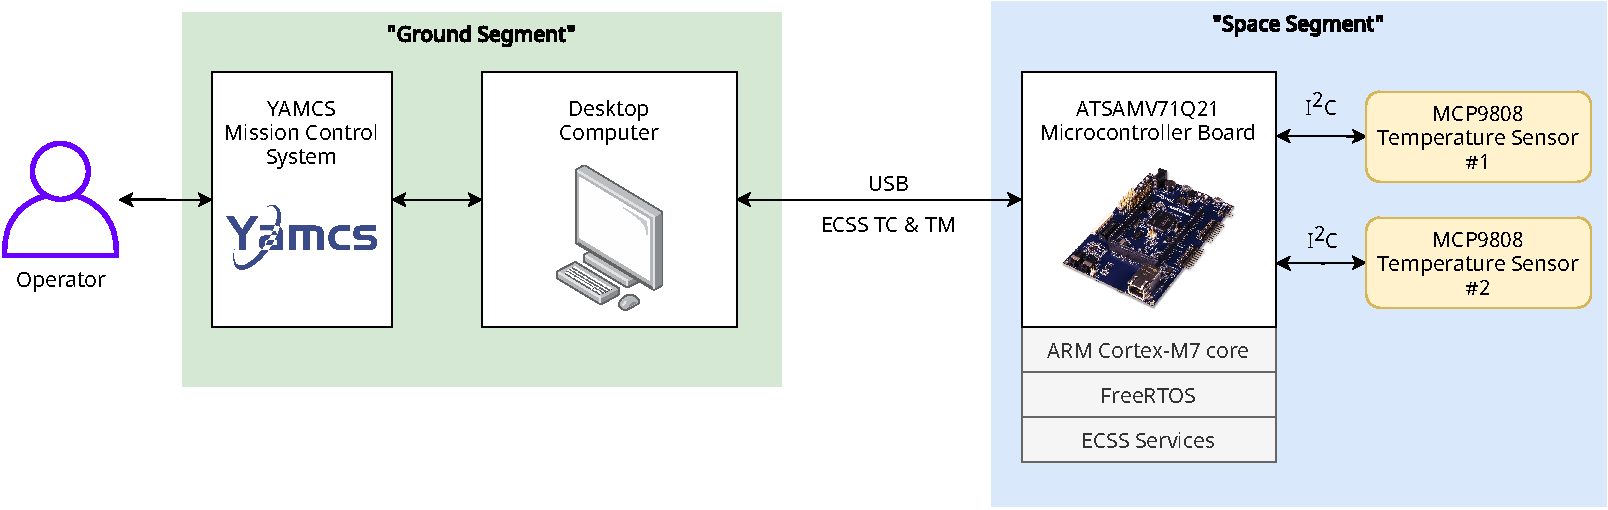
\includegraphics{SystemDescription}
	\caption{High-level block diagram of the demonstration system}
	\label{fig:block}
\end{figure*}

\pagebreak[4]
\section{System Description}

\subsection{Functionality}
\label{sec:tsvcd}

In order to emulate the most core functions of a spacecraft subsystem, we implemented a system with a single functional requirement:
\begin{quote}
	\texttt{RQ-010}: The system shall measure and report the ambient temperature.
\end{quote}

In order to justify implementing an \ac{FDIR} approach for this system, we will introduce a reliability requirement:
\begin{quote}
	\texttt{RQ-020}: No single failure on any measuring component shall lead to loss of system functionality.
\end{quote}

The detailed design of this simple demonstration system is presented in the following sections, and was architected to match the functionality, interfaces, design and software of the AcubeSAT nanosatellite as much as possible.

\subsection{Hardware}

The centre of the demonstration system is the \ac{MCU} used to simulate the design and functionality of one of AcubeSAT's subsystems (\Cref{sec:obdh}). The selected \ac{MCU} is the Atmel \texttt{ATSAMV71Q21} hosted on the \foothref{https://www.microchip.com/Developmenttools/ProductDetails/ATSAMV71-XULT}{\texttt{ATSAMV71-XULT}} development board. This \ac{MCU} is functionally identical to the one that will be used in orbit, featuring a 32-bit ARM Cortex-M7 core with \SI{2}{\mebi\byte} of flash and \SI{384}{\kibi\byte} of \acs{SRAM} memory, and a maximum clock speed of \SI{300}{\mega\hertz}.

\begin{figure}
	\centering
	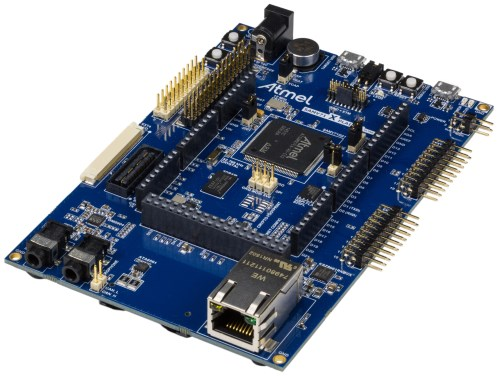
\includegraphics[width=.7\textwidth]{atsamv71xult}
	\caption{Manufacturer's photo of the \texttt{ATSAMV71-XULT} development board}
\end{figure}

\begin{figure}
	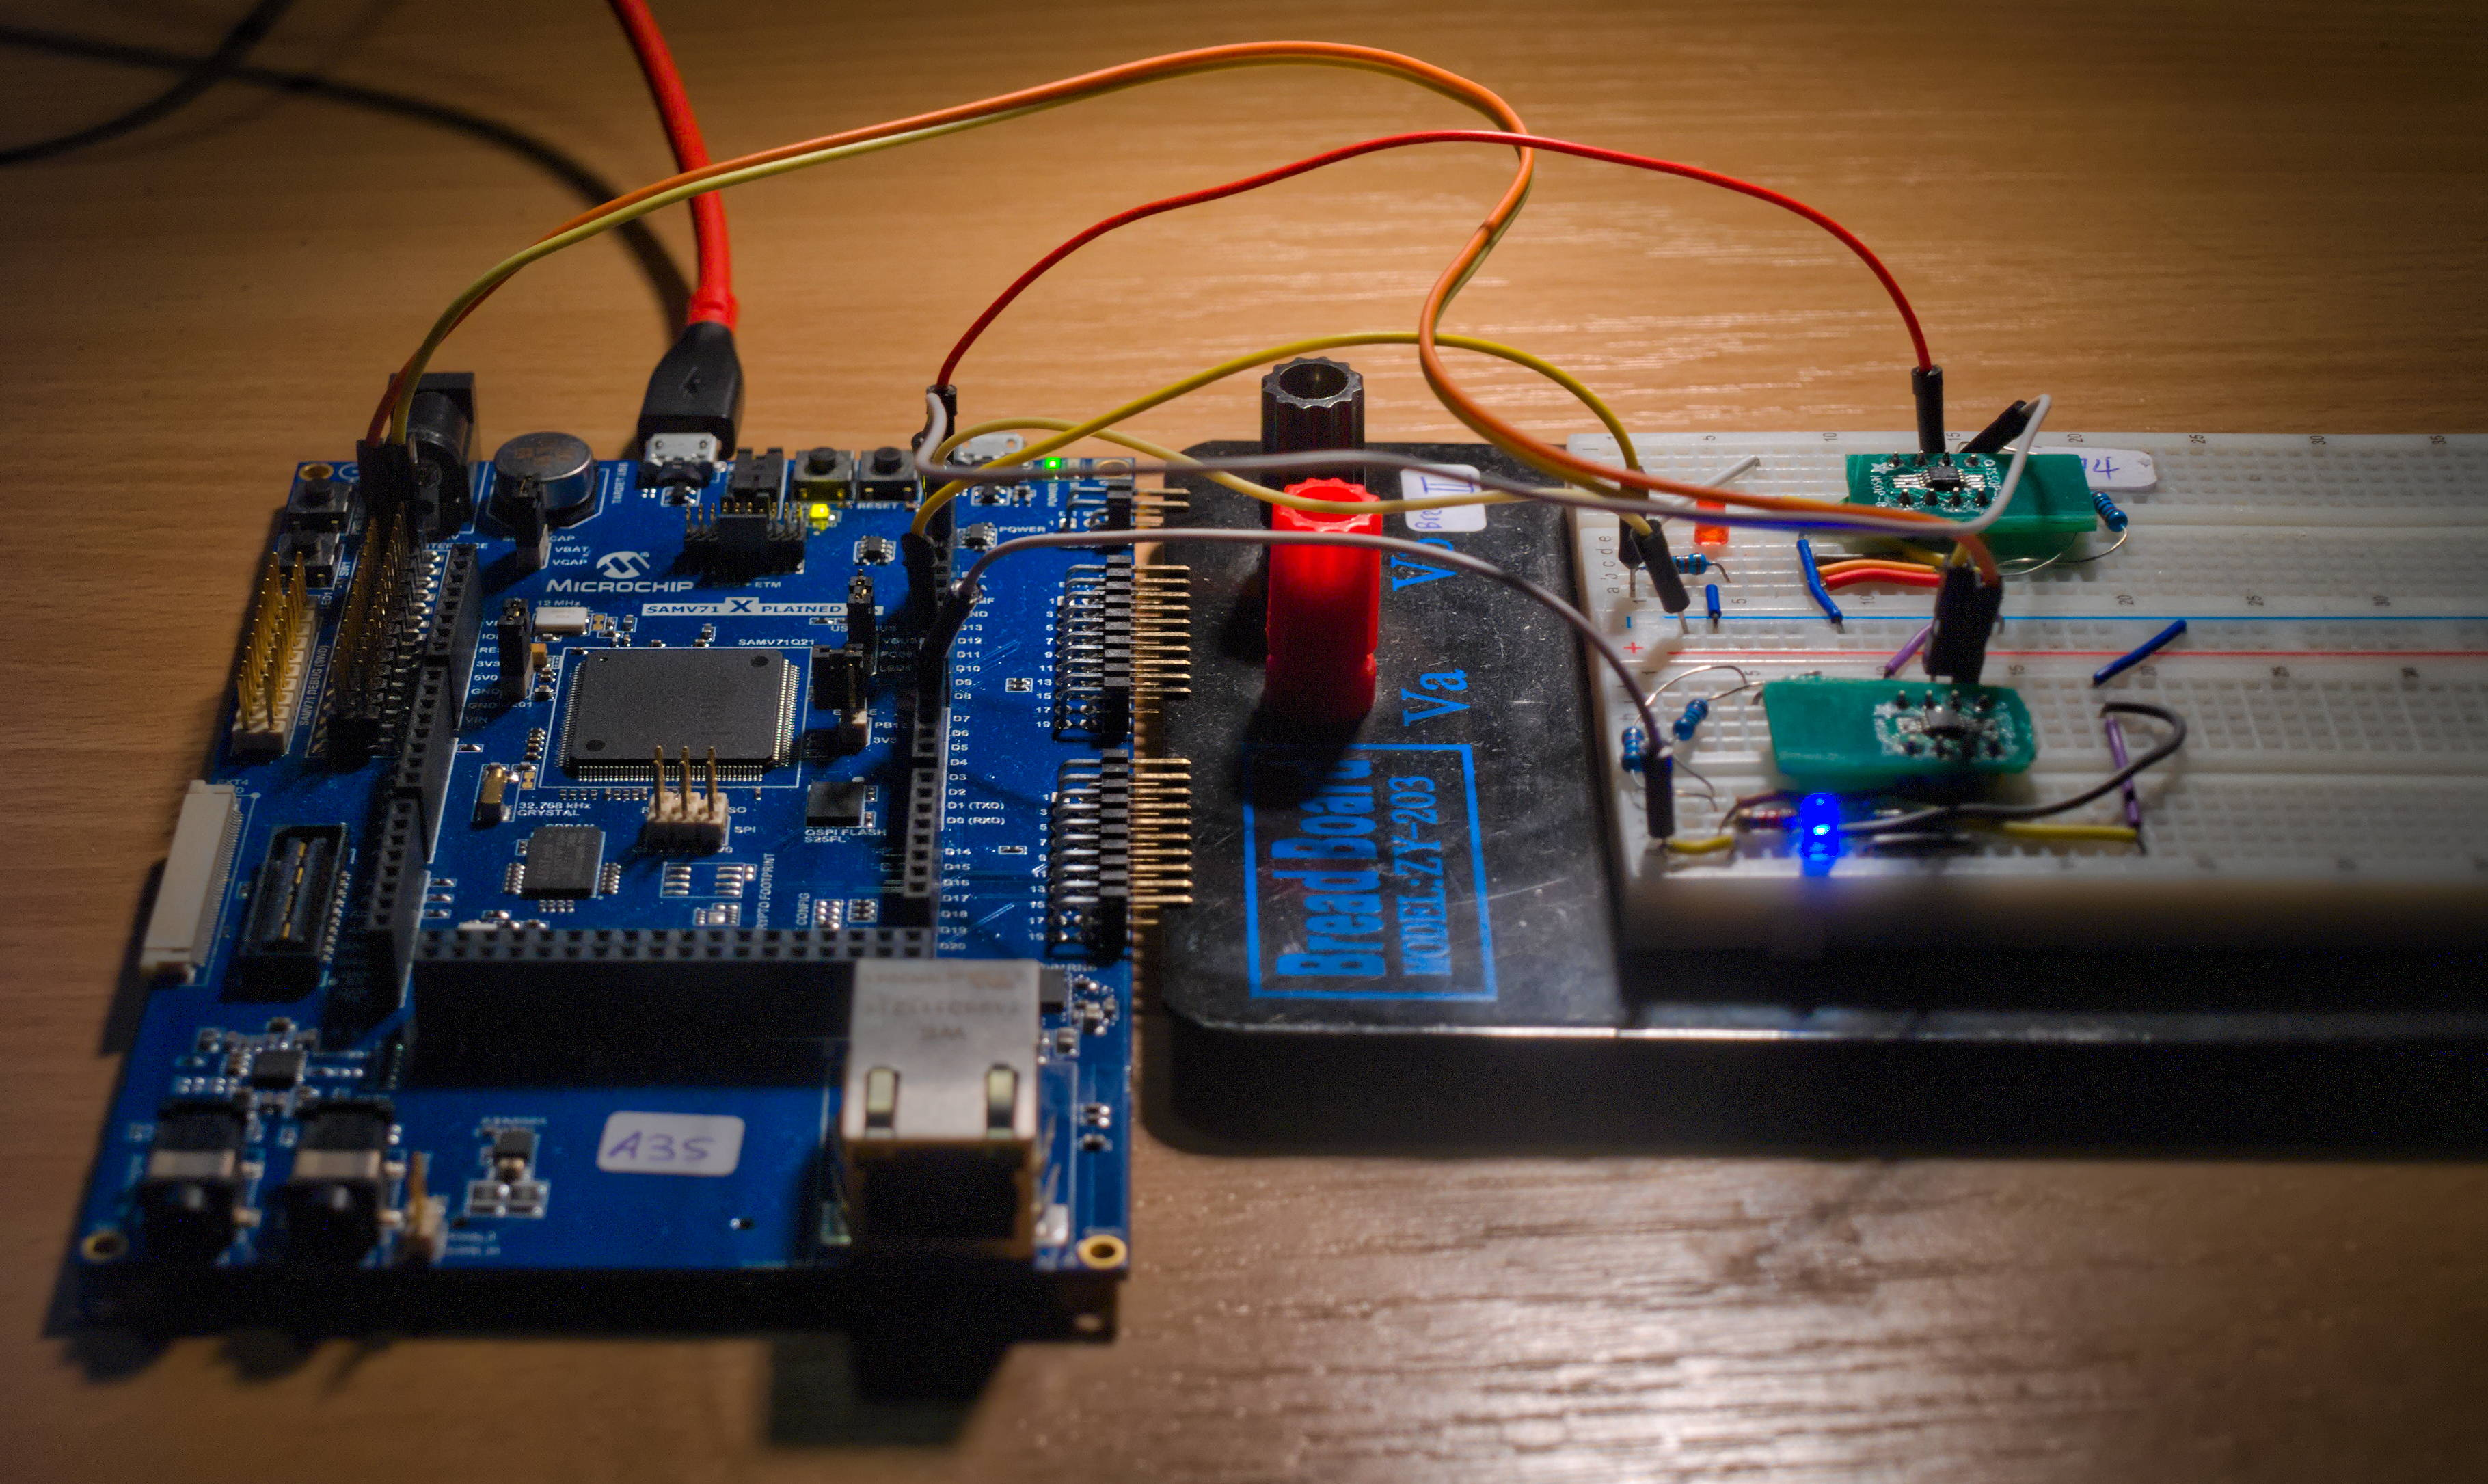
\includegraphics{test-system}\par
	\vspace*{3ex}
	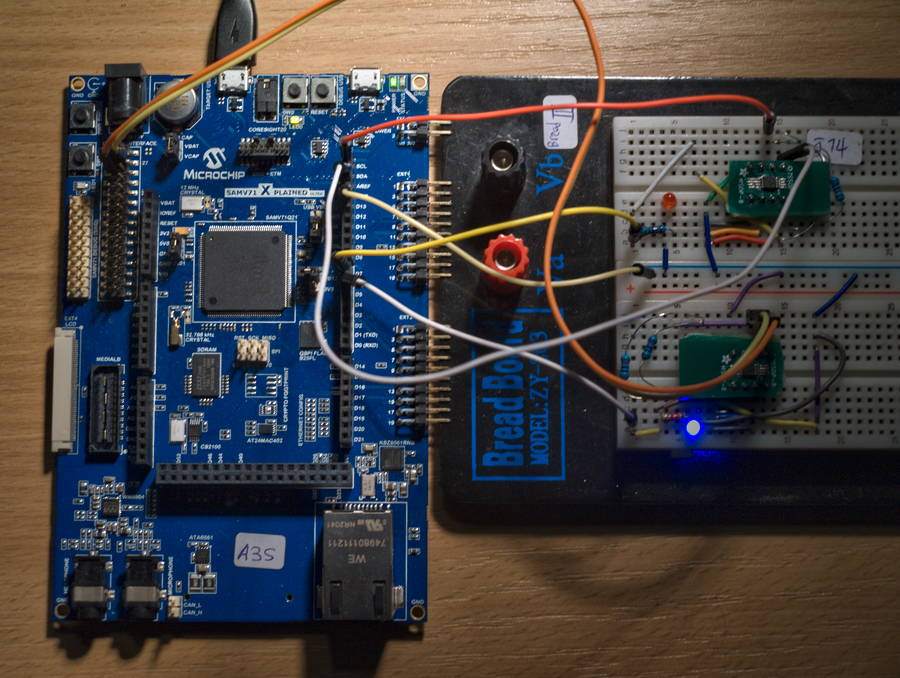
\includegraphics{system_top}
	\caption[The complete development system]{The complete development system. On the left is the blue development board of the \acs{MCU}. On the right is the breadboard housing the two temperature sensors. The cabling between the breadboard and the \acs{MCU} can also be discerned. The two installed \acsp{LED} show if the adjacent component is receiving power or not.}
\end{figure}
\acuse{LED}

\begin{marginfigure}
	      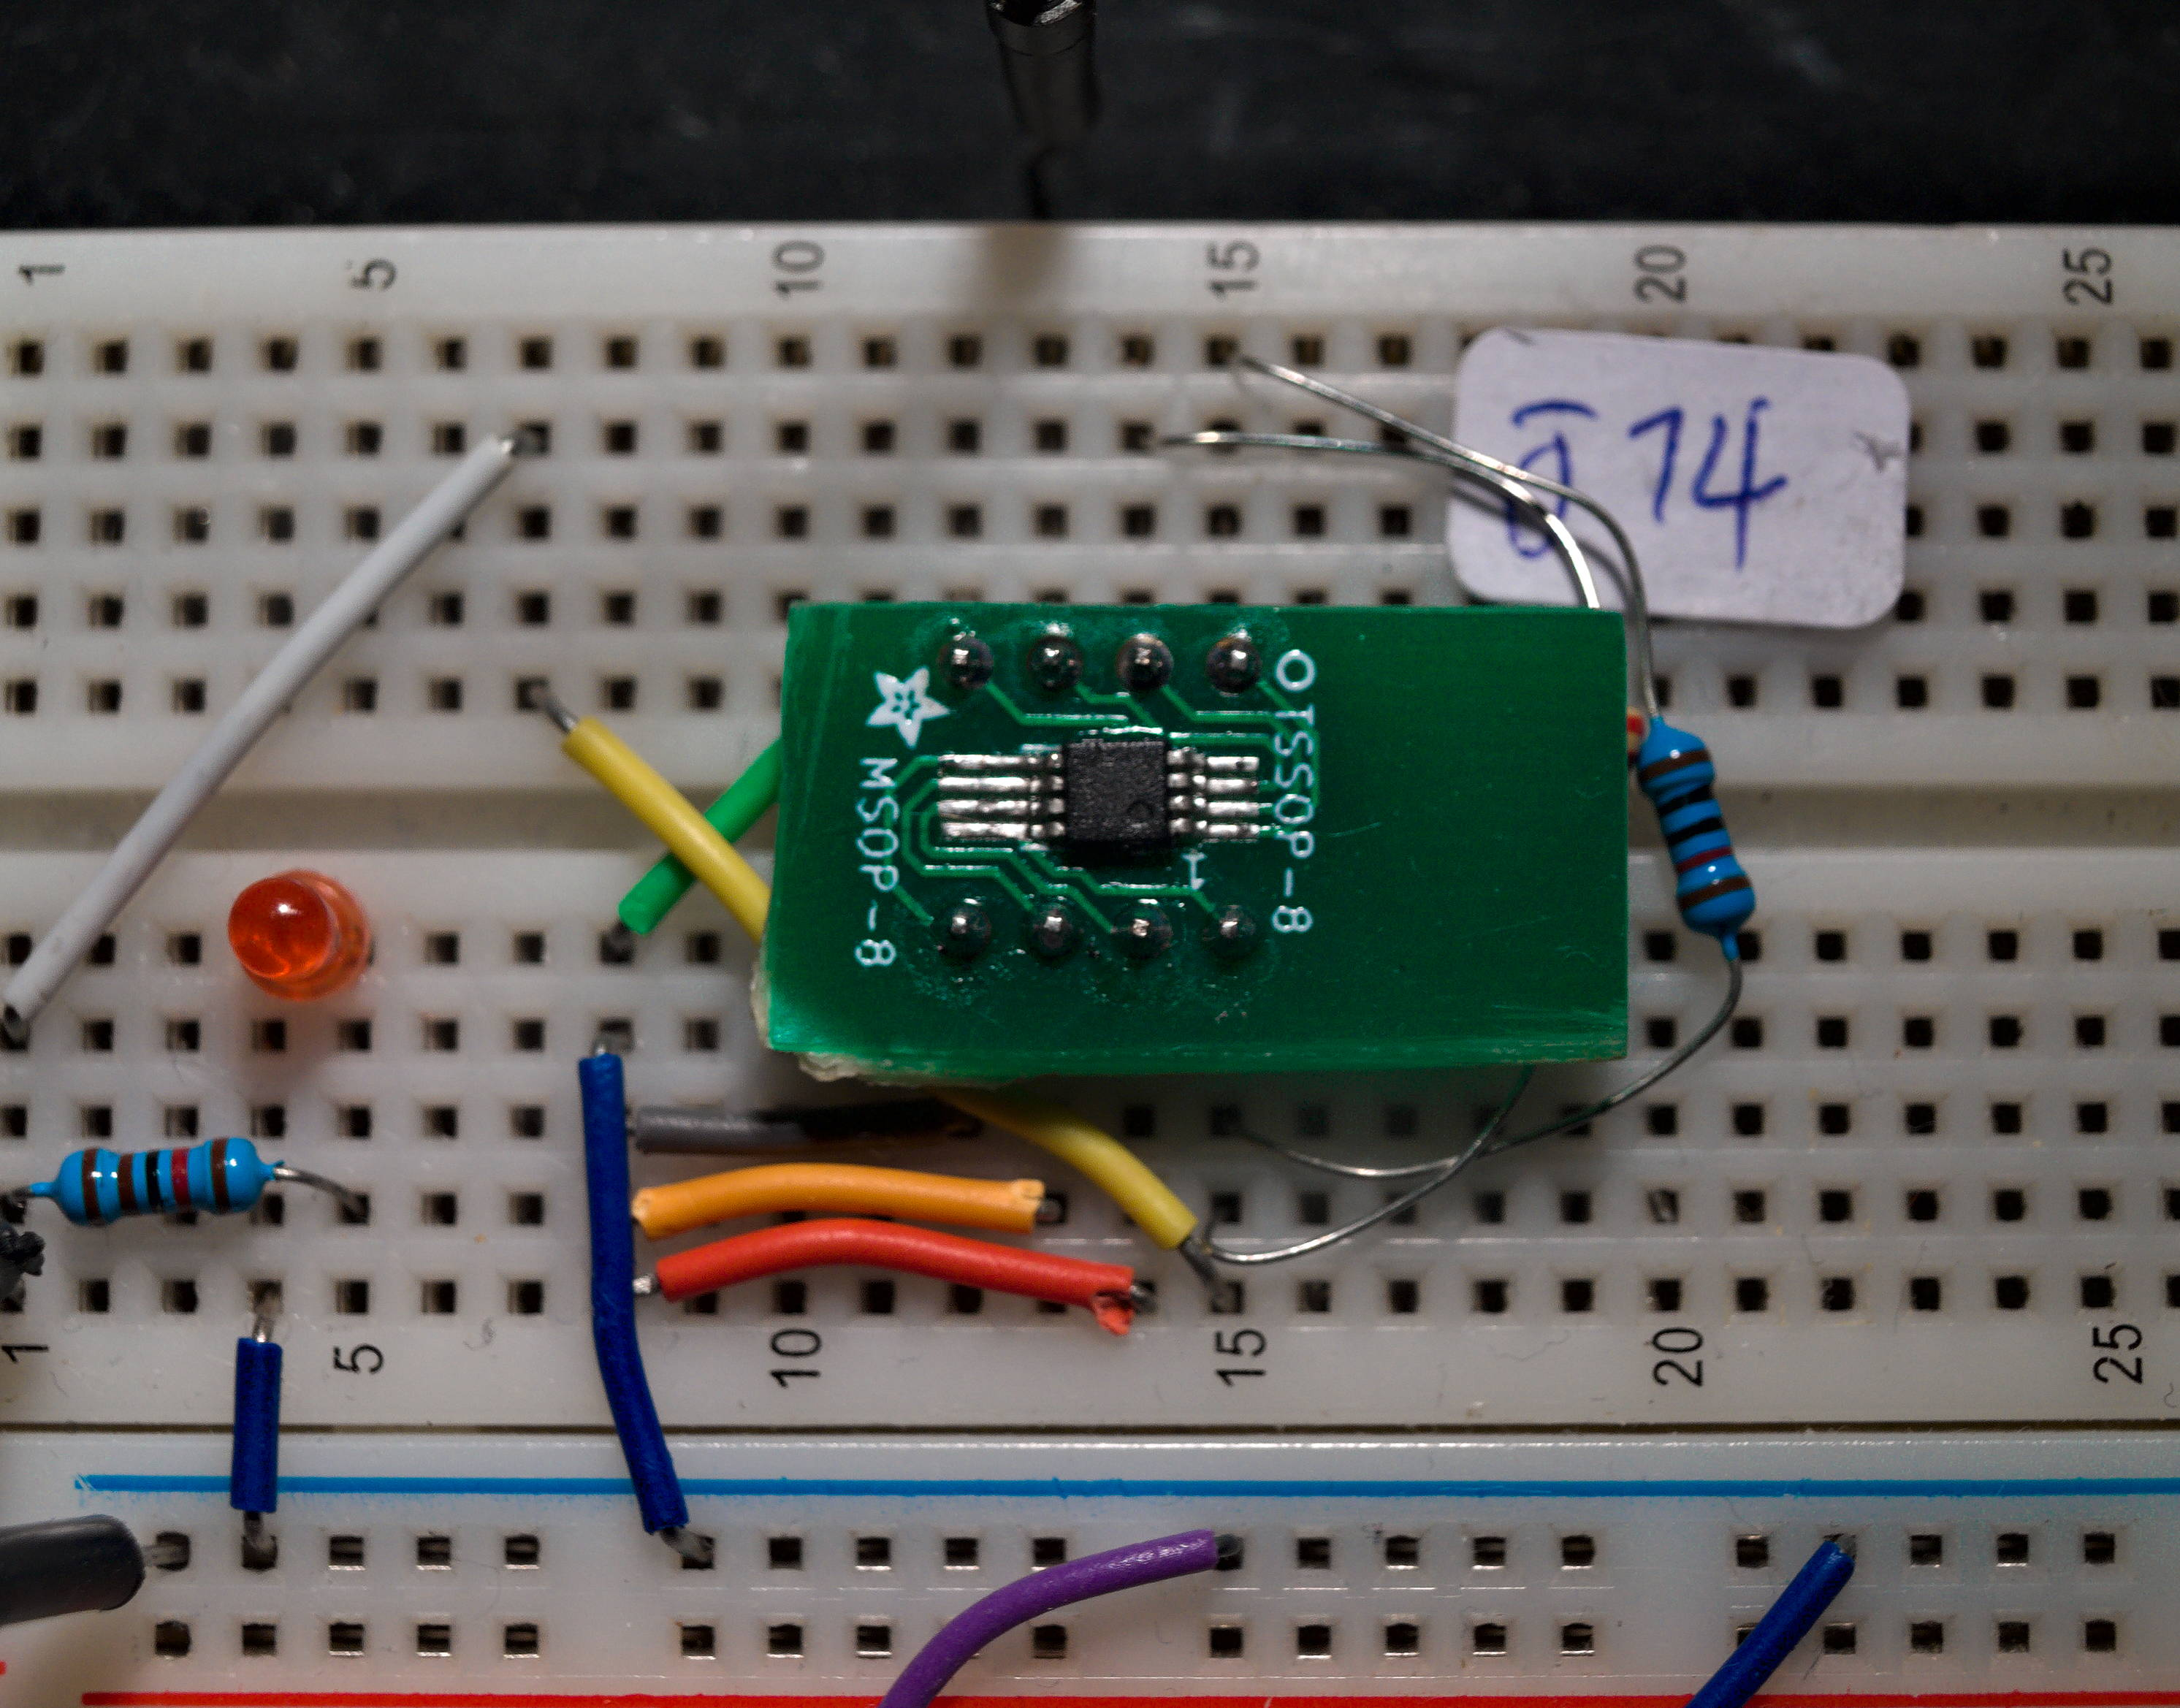
\includegraphics{mcp9808}
	      \caption{The MCP9808 temperature sensor, soldered onto the breakout \acs{PCB}}
\end{marginfigure}

The \ac{MCU} is accompanied by two \textbf{temperature sensors} which are used to simulate subsystem components that are prone to failure. The selected sensor is the Microchip \foothref{https://www.microchip.com/wwwproducts/en/MCP9808}{\texttt{MCP9808}} which offers an accurate and frequent temperature readout over an \ac{I2C} bus. The maximum acquisition interval for the sensor is \SI{250}{\milli\second}.

\marginnote{%
\textbf{Cold redundancy:} Only one component is operating, while the others are not.

\textbf{Warm redundancy:} One component is operating fully, and the others are operating with reduced functionality.

\textbf{Hot redundancy:} Two or more simultaneously active parts operate in parallel \autocite{SAVOIR-HB-003}.
}

The two sensors are wired in a \textbf{hot-redundant} configuration, allowed by their extremely low operating power. The two sensors are connected to different \ac{I2C} buses, so that the failure of one bus will not affect the operation of the other sensor.

\paragraph{\acs{USB} interface} In order to receive \acl{TM} and transmit \acl{TC} to the demonstrative space segment, a \acs{USB} link with a desktop computer is integrated into the design. This link uses the \acs{UART} peripheral of the microcontroller, which solely transfers \acs{ECSS} messages between the microcontroller and the desktop. These messages include the typical \acs{TM} reports and \acs{TC} requests, but also textual log messages intended for diagnostic purposes.

As the \acs{UART} protocol does not offer packetisation facilities by default, \ac{COBS} encoding \autocite{cheshire_consistent_overhead_1997} is implemented for all transmitted messages.

\paragraph{Connections}
The development board and sensors were laid out and connected directly. The sensor \acp{IC} were soldered on breakout \acp{PCB} which were manufactured based on Jaroslav Sýkora's design.\footnote[][-2ex]{\url{https://bit.ly/3vZwuh1}}

The electrical schematic of the implementation is shown in \Cref{fig:schematic}.
The two sensors are wired via \ac{I2C} with the necessary pull-up resistors. Their power is controlled directly by microcontroller outputs, allowing the user to completely cut the power of the sensors if needed. The \texttt{A} pins of the sensors are arbitrarily set to select the \ac{I2C} address of each device. The same address was used, as the two \ac{I2C} buses are separate.

\begin{figure*}[h]
	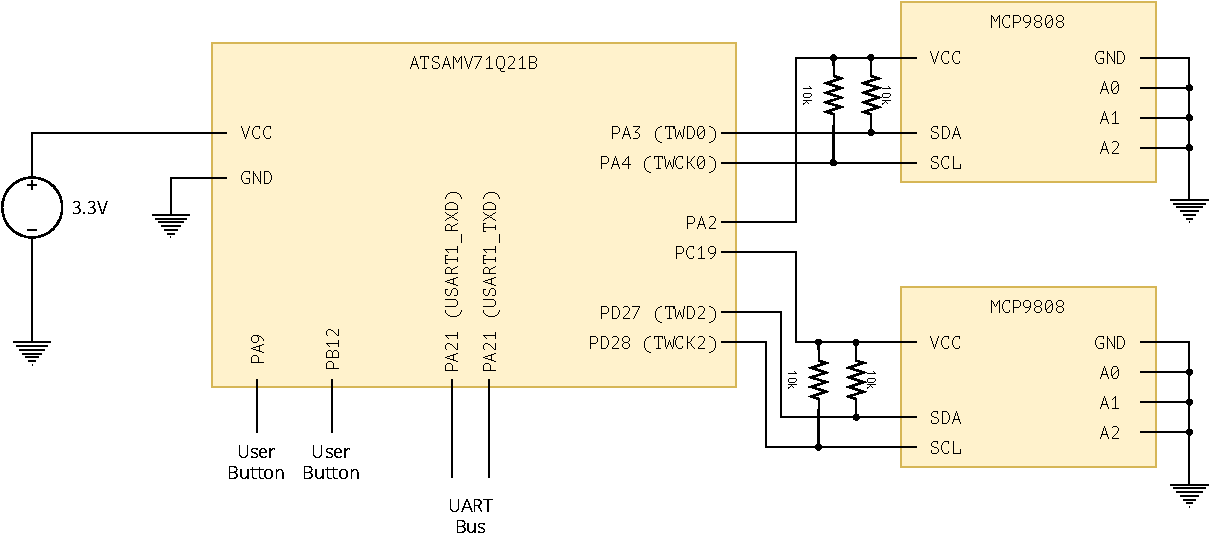
\includegraphics{ElectricalSchematic}
	\caption[Simplified electrical schematic of the implementation]{Simplified electrical schematic of the implementation. Decoupling capacitors, crystals and other boilerplate components are not shown, as they are already included in the \ac{MCU} development board.}
	\label{fig:schematic}
\end{figure*}

\FloatBarrier
\section{Software}

\subsection{Flight Segment}

All \ac{FDIR} operations and functionality are developed using the \textbf{C++} language\footnote{The \texttt{C++17} standard has been selected} on the \ac{MCU}. All developments rely on free and open source software which is freely available for download and modification. \foothref{https://git-scm.com/}{Git} version control is used for all software projects.

The \ac{FDIR} functionality is structured around the \textbf{ECSS-E-ST-70-41C \ac{PUS} implementation created by the AcubeSAT team},\footnote{\url{https://gitlab.com/acubesat/obc/ecss-services}} which offers a modular implementation of the standard utilising modern C++.

The \ac{MCU} software and business logic are built on \foothref[,]{https://www.freertos.org/}{\textbf{Free\acs{RTOS}}} a low-footprint real-time operating system targeted towards embedded devices. FreeRTOS provides the capability of safe concurrency, along with support for well-controlled tasks and a number of synchronisation primitives.

\begin{table*}[h]
	\centering
	\caption[][5pt]{List of Free\acs{RTOS} tasks implementing the experimental setup}
	\label{tab:rtos-tasks}
	\renewcommand{\arraystretch}{1.5}
	\begin{tabularx}{\textwidth}{@{}llX@{}}
		\toprule
		Name & Stack size & Description \\ \midrule
		\texttt{Internal\_Temp} & \SI{2.5}{\kilo\byte} & Receives diagnostic measurements from the internal \acs{MCU} temperature sensor, and blinks an \acs{LED} for observability purposes \\
		\texttt{ECSS} & \SI{3}{\kilo\byte} & Executes the periodic processes dictated by the \acs{ECSS} services. This includes beacon transmission and evaluation of the on-board monitoring definitions. This task essentially implements \acs{FDIR}. \\
		\texttt{\acs{UART}\_Tx} & \SI{3}{\kilo\byte} & Transmission of \acs{UART} messages to the computer. This task works as a ``gatekeeper task'', and is the only one that can send \acs{UART} messages. All other tasks communicate with this one via a Free\acs{RTOS} stack. \\
		\texttt{\acs{UART}\_Rx} & \SI{6}{\kilo\byte} & Reception of \acs{UART} messages from the computer. For simplicity, this task is also responsible for the execution of such received commands. \\
		\texttt{T1} & \SI{1.5}{\kilo\byte} & Communication with temperature sensor \#1 and update of relevant \acs{ECSS} parameters \\
		\texttt{T2} & \SI{1.5}{\kilo\byte} & Communication with temperature sensor \#2 and update of relevant \acs{ECSS} parameters \\ \bottomrule
	\end{tabularx}
\end{table*}

To ensure high reliability and a low resource footprint of the software, the following \textbf{constraints} are enacted in C++ development:
\begin{compactenum}
	\item Dynamic memory allocation\footnote{Use of \mintinline{cpp}{malloc}, \mintinline{cpp}{new} etc.} is banned completely from the code.
	\label{itm:malloc}
	\item \Cref{itm:malloc} means that standard C++ containers cannot be used. Instead, the \foothref{https://www.etlcpp.com/}{\acf{ETL}} is integrated in the software.
	\item ``Expensive'' features such as Run-Time Type Inference, Dynamic Casts or Exceptions are also prohibited.
\end{compactenum}

The \href{https://www.microchip.com/en-us/development-tools-tools-and-software/embedded-software-center/mplab-harmony-v3}{MPLAB Harmony}\footnote[][1.5cm]{\url{https://www.microchip.com/en-us/development-tools-tools-and-software/embedded-software-center/mplab-harmony-v3}} \ac{HAL} and configurator are used to interface with all the \acs{MCU}'s peripherals. \foothref{https://www.jetbrains.com/clion/}{CLion} has been selected as the \acs{IDE}, along with the \foothref{https://cmake.org/}{CMake} build system.

All software developed in the scope of this thesis is available online, and listed in \Cref{tab:new_software}. A summary of used libraries can also be found in \Cref{tab:old_software}.

\begin{figure*}[h]
	\vspace{1cm}
	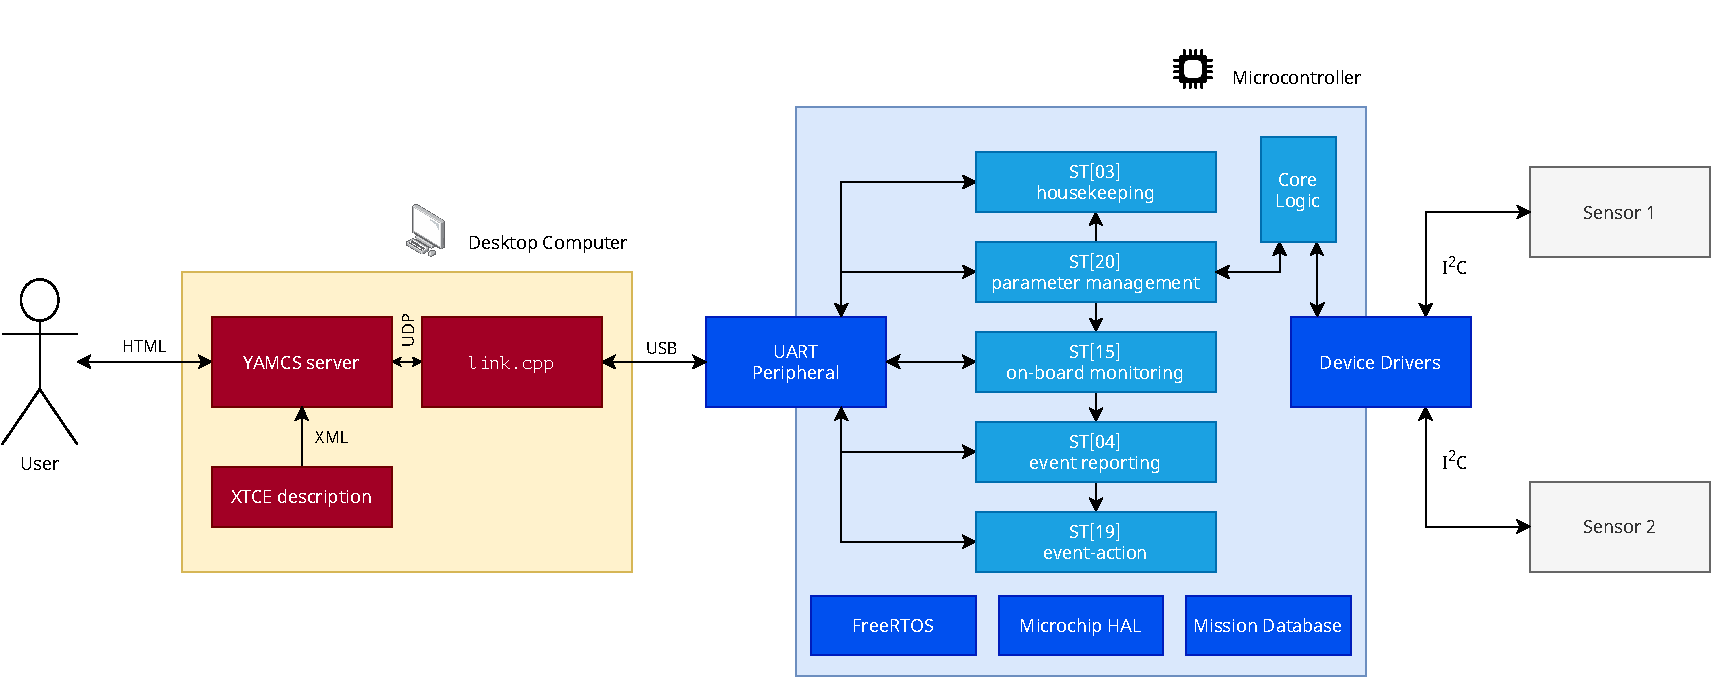
\includegraphics{SoftwareFlow}
	\caption{View of the software components and the data flow between them}
	\label{sec:softwareflow}
\end{figure*}

\FloatBarrier
\begin{table*}[h]
	\centering
	\caption[][5pt]{List of new software developed for this thesis}
	\renewcommand{\arraystretch}{1.2}
	\label{tab:new_software}
	\begin{tabularx}{\textwidth}{@{}lXp{6cm}@{}}
		\toprule
		Library name & Description & URL \\ \midrule
		\textbf{\texttt{fdir-demo}} & Full microcontroller code for the demonstration & \small \url{https://github.com/kongr45gpen/fdir-demo} \\
		\textbf{\texttt{fdir-demo-yamcs}} & Ground segment software: files and source code for \acs{YAMCS} integration and \acs{MCU} communications & \small \url{https://github.com/kongr45gpen/fdir-demo-yamcs} \\
		\bottomrule
	\end{tabularx}
\end{table*}

\begin{table*}[h]
	\centering
	\caption[][5pt]{List of used ``off-the-shelf'' software libraries}
	\renewcommand{\arraystretch}{1.5}
	\label{tab:old_software}
	\vspace{1.3cm}
	\begin{tabularx}{\textwidth}{@{}lp{6cm}X@{}}
		\toprule
		Library name & Description & Modifications \\ \midrule
		\href{https://www.freertos.org/}{FreeRTOS} & Real-time operating system for embedded devices & \\
		\href{https://gitlab.com/acubesat/obc/ecss-services}{\texttt{ecss-services}} & C++ implementation of the ECSS-E-ST-70-41C \acl{PUS} %\autocite{ECSS-E-ST-70-41C} 
		& \small Missing services were implemented and some interface improvements were made to improve integration with the \acs{MCU}\newline\small\url{https://gitlab.com/kongr45gpen/ecss-services/-/tree/fdir}
		 \\
		 \href{https://www.etlcpp.com/}{\acs{ETL}}  & C++ library (including containers, algorithms and other utilities) for applications with embedded constraints &
		 \\
 		\href{https://github.com/yamcs/yamcs}{\acs{YAMCS}}  & Software framework for mission \& spacecraft control & %\autocite{cheshire_consistent_overhead_1997}
 		\\
		\href{https://github.com/cmcqueen/cobs-c}{\texttt{cobs-c}}  & Implementation of \ac{COBS} %\autocite{cheshire_consistent_overhead_1997}
		 & \\
		 \href{https://getmdl.io/}{Material Design Lite} & CSS style framework (for \acs{GS} interface) & \\
		 \href{https://lodash.com/}{\texttt{lodash}} & Javascript utility functions (for \acs{GS} interface) & \\
		\bottomrule
	\end{tabularx}
\end{table*}


\FloatBarrier
\subsection{Software Size}

Since we are developing an embedded system with limited resources, it makes sense to analyse the size of the generated code. The \texttt{gcc} compiler allows measuring the memory consumption of the software in detail. The total size of the software is shown in \Cref{tab:resusage}, and the C++ files with the largest footprint are shown in \Cref{tab:ramusage,tab:romusage}.\footnote{The data was generated using the \href{https://github.com/PromyLOPh/linkermapviz}{\texttt{linkermapviz}} library.}


\begin{table}[h]
	\centering
	\caption{Generated code size with different compiler options}
	\label{tab:resusage}
	\begin{tabular}{@{}llll@{}}
		\toprule
		\multicolumn{4}{l}{No optimisation (\texttt{-O0})} \\ \midrule
		Memory type &        Used & Total &  Percentage \\[1ex]
		\acs{ROM}   &   \SI{254324}{\byte}   &    \SI{  2}{\mega\byte} &     12.13\% \\
		\acs{RAM}   &   \SI{205992}{\byte}   &    \SI{384}{\kilo\byte} &     52.39\% \\ \midrule
		\multicolumn{4}{l}{Optimise for size (\texttt{-Os})} \\ \midrule
		Memory type &        Used & Total &  Percentage \\[1ex]
		\acs{ROM}   &   \SI{228384}{\byte}   &    \SI{  2}{\mega\byte} &     10.89\% \\
		\acs{RAM}   &   \SI{205992}{\byte}   &    \SI{384}{\kilo\byte} &     52.39\% \\ \bottomrule
	\end{tabular}
	\vspace{2ex}
\end{table}

\begin{table}[h]
	\centering
	\caption[List of files with highest ROM usage]{List of files with highest \acs{ROM} usage (excluding system libraries)}
	\label{tab:romusage}
	\begin{tabularx}{\textwidth}{@{}S[table-format=5.0]X@{}}
		\toprule
		\multicolumn{1}{r}{Size (\si{\byte})} & File \\ \midrule
		22515 & \texttt{ServicePool.cpp} \\
		12350 & \texttt{main.cpp} \\
		9271 & \texttt{TimeBasedSchedulingService.cpp} \\
		8684 & \texttt{SystemParameters.cpp} \\
		7708 & \texttt{EventActionService.cpp} \\
		6546 & \texttt{OnBoardMonitoringService.cpp} \\
		5952 & \texttt{ECSSTask.cpp} \\
		4451 & \texttt{FreeRTOS\_tasks.c} \\
		4404 & \texttt{MCP9808-internal.cpp} \\
		3281 & \texttt{Logger.cpp} \\
		\bottomrule
	\end{tabularx}
\end{table}

\begin{table}[h]
	\centering
	\caption[List of files with highest RAM usage]{List of files with highest \acs{RAM} usage (excluding system libraries)}
	\label{tab:ramusage}
	\begin{tabularx}{\textwidth}{@{}S[table-format=5.0]X@{}}
		\toprule
		\multicolumn{1}{r}{Size (\si{\byte})} & File \\ \midrule
		131104 & \texttt{heap\_4.c} \\
		38088 & \texttt{ServicePool.cpp} \\
		11192 & \texttt{UARTTask.cpp} \\
		1064 & \texttt{SystemParameterMonitoring.cpp} \\
		340 & \texttt{UARTRXTask.cpp} \\
		260 & \texttt{FreeRTOS\_tasks.c} \\
		200 & \texttt{sys\_time.c} \\
		188 & \texttt{SystemParameters.cpp} \\
		50 & \texttt{main.cpp} \\
		\bottomrule
	\end{tabularx}
\end{table}


Note that no attempts were made to manually optimise the memory consumption or the performance of the system. Also, note that due to the usage of the \acs{ETL} library and the ban on dynamic memory allocation, the values shown in \Cref{tab:ramusage} refer to the majority of runtime \acs{RAM} consumption. In fact, the stack used by all Free\acs{RTOS} tasks is already listed as part of the \texttt{heap\_4.c} file.

\FloatBarrier
\subsection{\ac{I2C} Failure Detection}

It is of interest to investigate how the hardware \ac{I2C} peripheral provided by the microcontroller can be used to monitor the symptoms of bus failure.

\begin{enumerate}
	\item \textbf{Microcontroller peripheral errors}
	
	\marginnote{To ensure detection of peripheral errors, it is important to make sure that the error status of the peripheral is not discarded after every operation. Interrupts and the \href{https://en.cppreference.com/w/cpp/language/attributes/nodiscard}{\mintinline{cpp}{[[nodiscard]]}} C++ feature are used to ensure that all errors are caught.}
	The microcontroller's \ac{I2C} peripheral is capable of generating an error whenever \emph{the communicating peripheral does not set the ``acknowledge'' bit}. Failure to set this bit might be a result of disconnection of the clock or data lines, failure of the bus, or non-operation of the peripheral itself.
	
	\item \textbf{Response timeout}
	
	For some adverse \ac{I2C} bus conditions, such as incorrectly chosen pull-up resistor values or large amounts of capacitive load, \ac{I2C} signal integrity may be lost (\Cref{subfig:i2c_dirty}). This error is not detected by the microcontroller's peripheral directly, but can be diagnosed by adding a timeout to the sensor's data readouts.
	
	\item \textbf{Chip ID}
	
	\begin{margintable}
		\centering
		\caption{Read-only registers for the MCP9808}
		\label{tab:mcp9808readonly}
		\begin{tabularx}{\linewidth}{@{}lXl@{}}
			\toprule
			Address & Register Name & Value \\ \midrule
			\texttt{0x06} & Manufacturer ID & \texttt{0x0054} \\
			\texttt{0x07} & Device ID & \texttt{0x0400} \\ \bottomrule
		\end{tabularx}
	\end{margintable}
	
	It is possible that the sensor suffers a severe fault but is still able to respond to \ac{I2C} commands or set the \emph{acknowledge} bit. For this reason, a more rigid check of the sensor's status is performed before each temperature read: the \emph{permanently-set} registers of the peripheral contain values which, under nominal conditions, are hard-coded and will not change, barring hardware failure. If any value other than the expected one is returned, the peripheral or the bus are assumed to have a fault.
\end{enumerate}

\begin{figure}[h]
	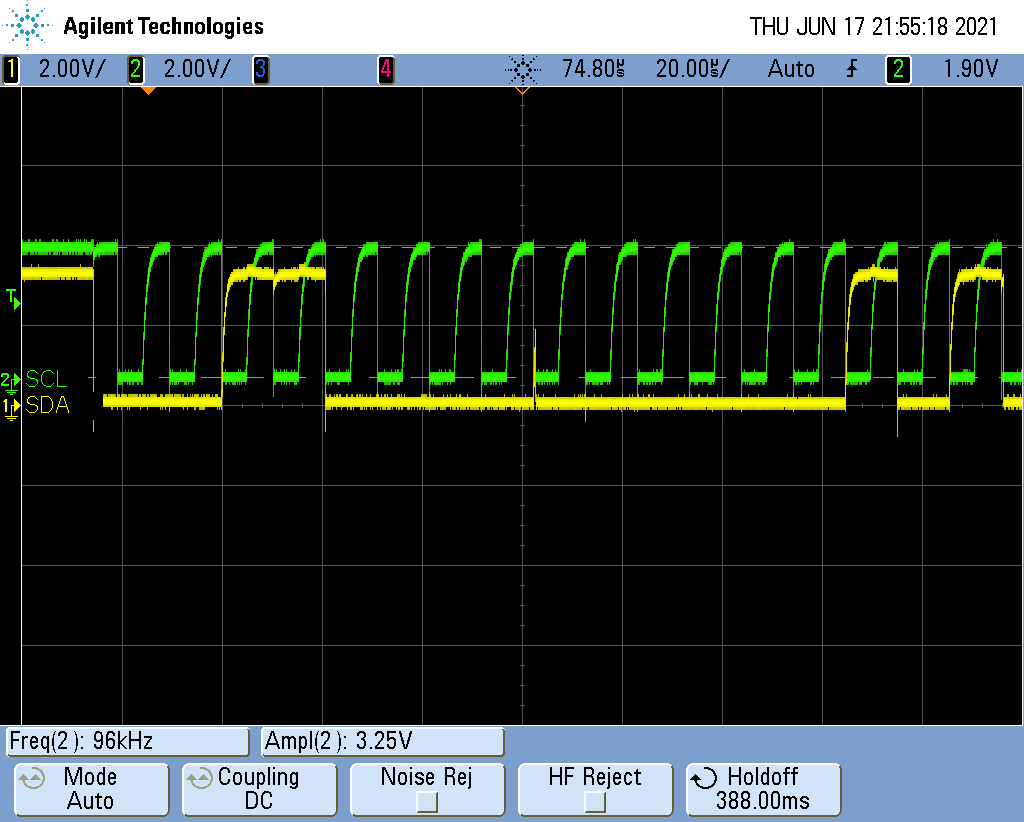
\includegraphics[trim={0 10cm 0 1.8cm},clip]{scope_1}
	\label{subfig:i2c_clean}
	\caption[Clear I2C signal]{Clear \acs{I2C} signal. The green \acs{SCL} waveform has a shape where it is easy to identify each clock pulse, and the data of the yellow \acs{SDA} signal can be easily cross-referenced with the clock. The amplitude of the signals is approximately \SI{3.3}{\volt}.}
\end{figure}

\begin{figure}[h]
	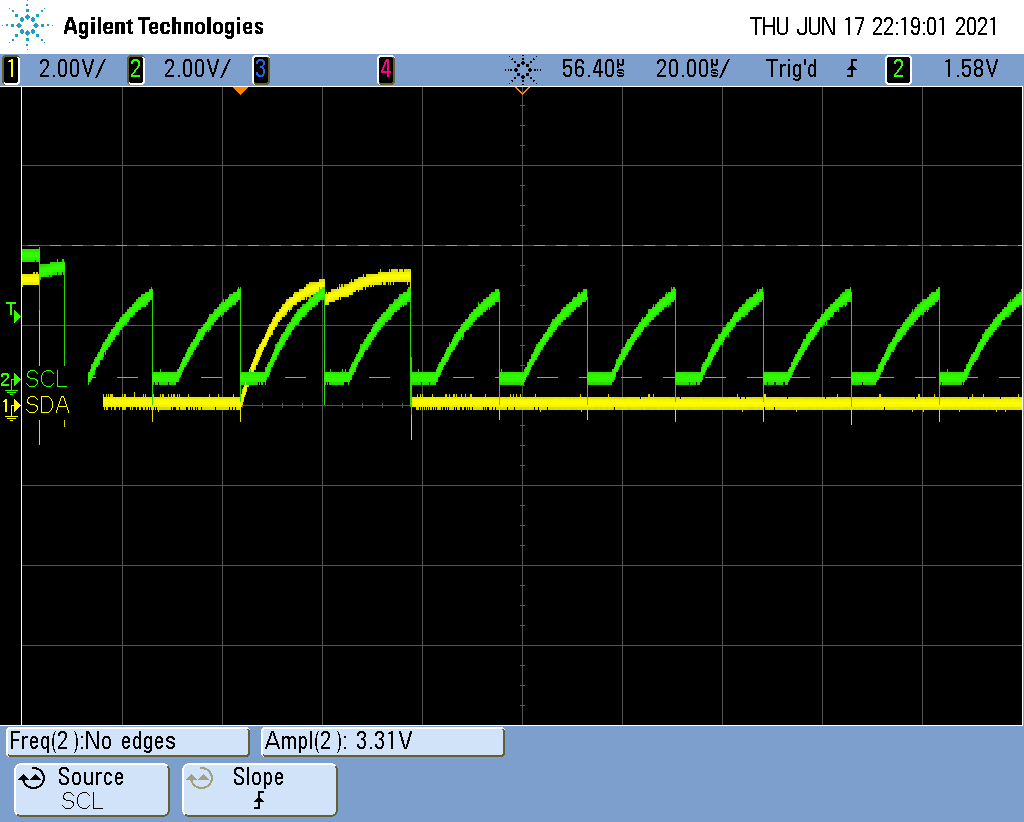
\includegraphics[trim={0 10cm 0 1.8cm},clip]{scope_5}
	\caption[Faulty I2C signal]{Faulty \acs{I2C} signal, when there is a large capacitive load on the \acs{I2C} network. The rise time of both signals is prohibitively high, and communication in this case is not possible. The signal does not reach the \SI{3.3}{\volt} value. In this case, it is not possible to transmit data in the bus, and the component is considered to have failed.}
	\label{subfig:i2c_dirty}
\end{figure}

\FloatBarrier

\subsection{Mission Control}

The ground segment desktop computer needs to parse received packets and send commands, as well as display information about the sensor measurements, \ac{FDIR} status and health of the connected flight system.

The \acs{YAMCS} \autocite{sela_yamcs_lightweight_2012} framework was selected to cover the aforementioned needs, and has been tailored to provide the capabilities needed for this demonstration.

The \ac{ECSS} protocol \autocite{ECSS-E-ST-70-41C} is not supported by \acs{YAMCS} by default. However, the necessary commands have been integrated into the system using the supported \ac{XTCE} specification \autocite{simon_xtce_standard_2004}.

\begin{figure}[h]
	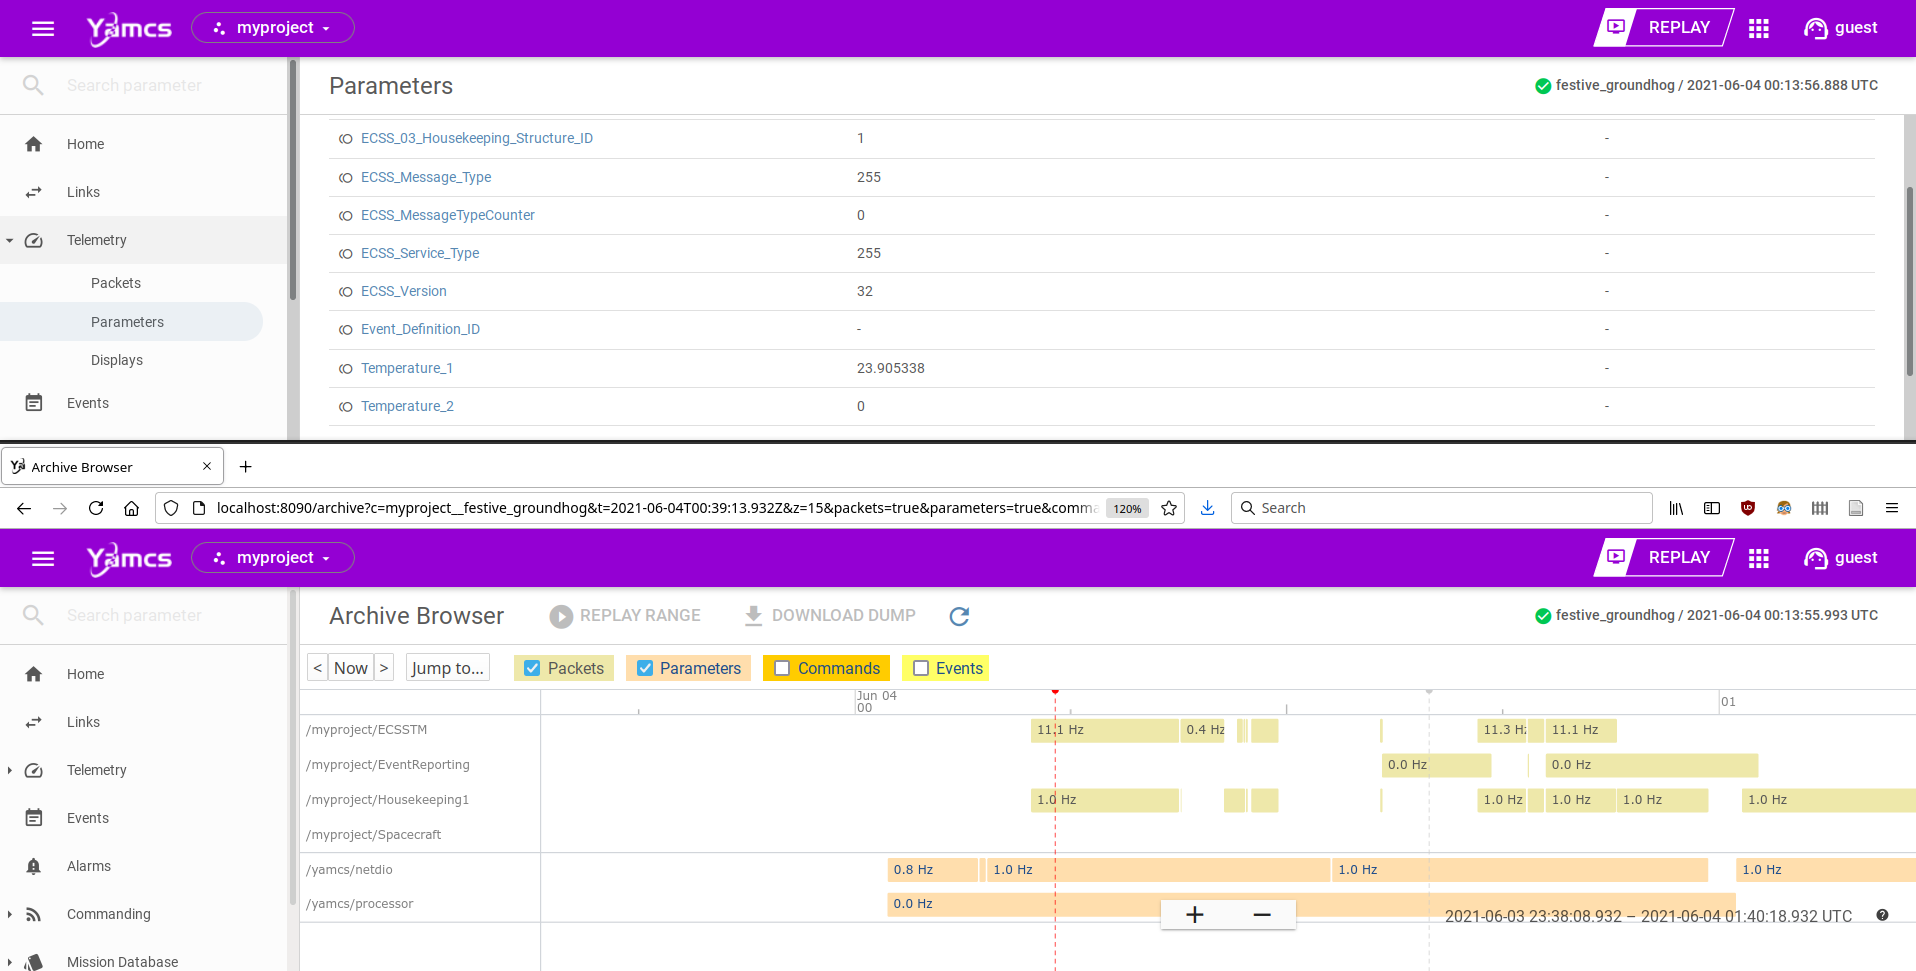
\includegraphics{screenshots/yamcs_replay}
	\caption{\acs{YAMCS} parameter and archive views}
	\setfloatalignment{b}
\end{figure}

\subsection{\acs{PUS} database}
\label{sec:pusinterface}
The \acs{YAMCS} suite does not provide built-in support for monitoring and controlling the satellite's \acs{PUS} database. This means that there is no convenient way to view \emph{events}, \emph{parameters}, \emph{monitoring} definitions and \emph{event-action} definitions.

\begin{figure*}[h]
	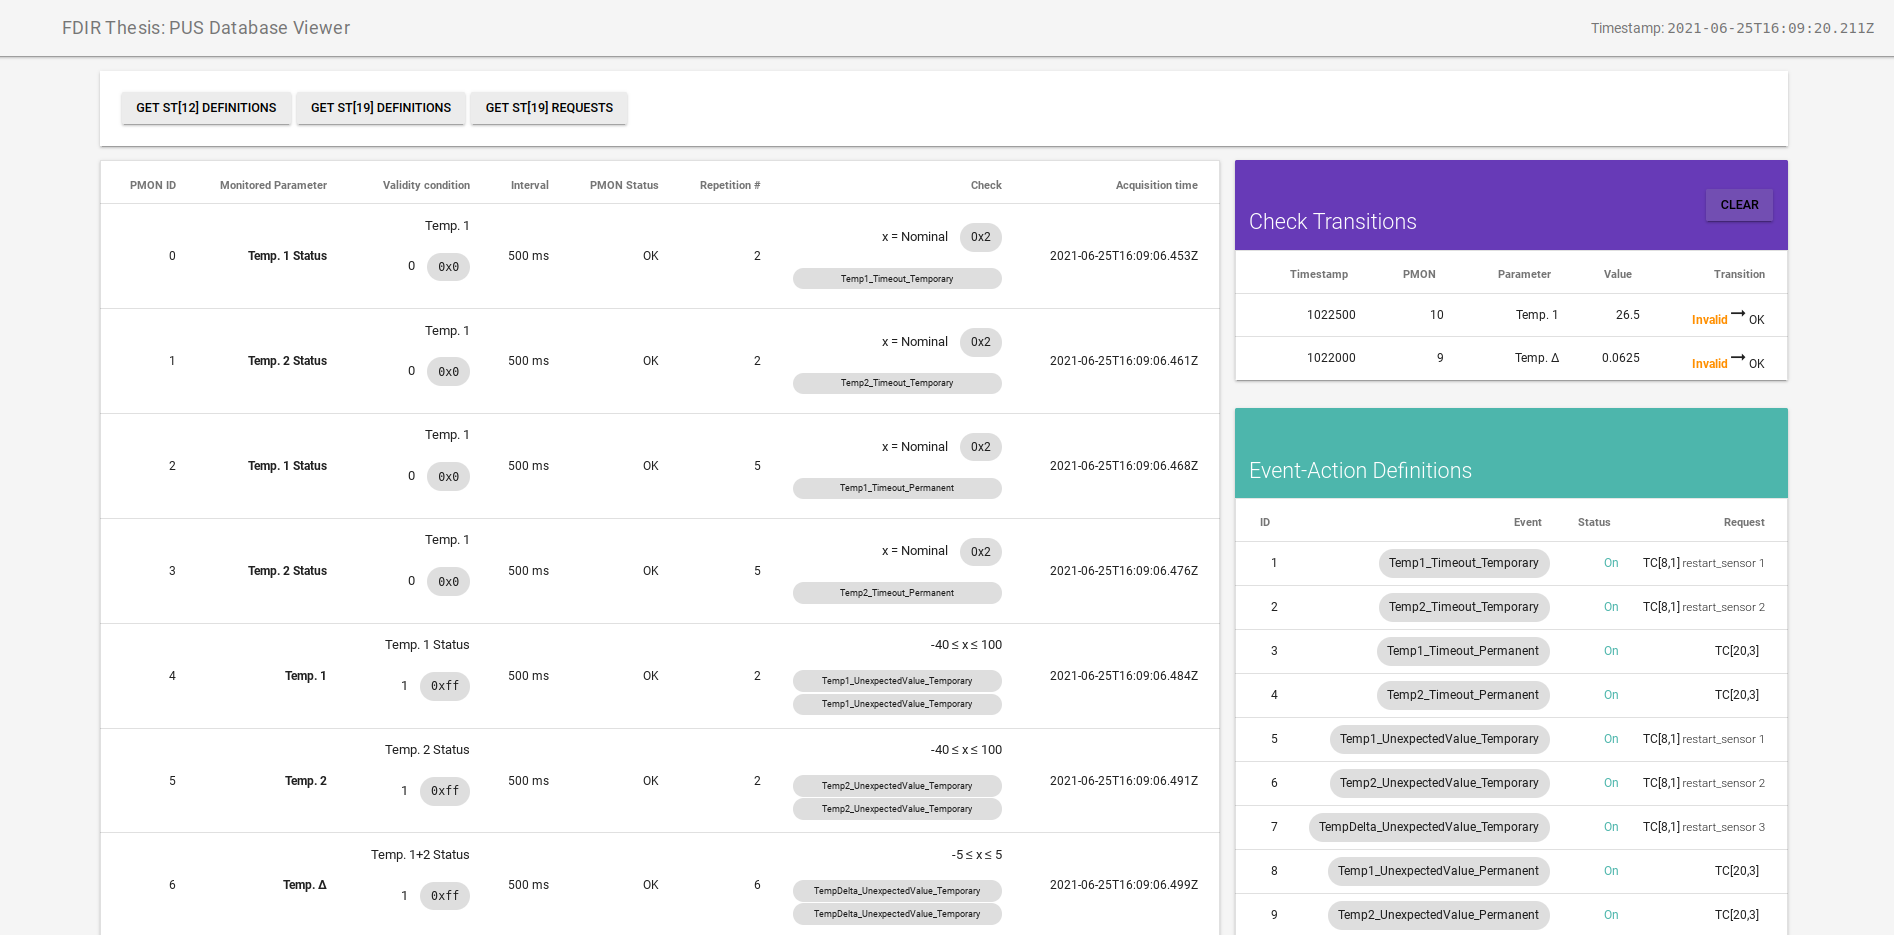
\includegraphics{screenshots/pus_viewer}
	\caption[The ``PUS database viewer'' interface]{The ``\acs{PUS} database viewer'' interface. On the left is the list of monitoring definitions, on the top right is the list of transitions, and on the bottom right is the list of event-action definitions.}
		\label{fig:pusviewer}
\end{figure*}
	
To allow for a quick overview of the \acs{FDIR} status, we implemented an online interface showing the above (\Cref{fig:pusviewer}). The interface is updated in real-time via the \acs{YAMCS} \acs{HTTP} \acs{API}, and displays both \acs{FDIR} definitions and live status.

The application was written in HTML and Javascript, taking advantage of the WebSocket technology, and its GUI is based on the Material Design Lite library.\footnote[]{\url{https://getmdl.io/}} It is located in the\foothref{https://github.com/kongr45gpen/fdir-demo-yamcs/tree/master/ecss-interface}{\texttt{fdir-demo-yamcs}} repository, along with the other parts of the demo \acl{GS}.

\section{\ac{FDIR} setup}

The purpose of the test setup is to observe the response of the system to any failure of the two ``vulnerable'' temperature sensors. For this purpose, we will attempt to simulate every failure mode of each sensor, and design an \ac{FDIR} implementation that anticipates all those failures.

\marginnote{Double failures are not investigated in the scope of this document, as they are mostly considered only for launchers and manned missions \parencite{SAVOIR-HB-003}.}
As a required input for the \ac{FDIR} detailed design, a \ac{FMEA} analysis needs to be prepared for the system. All \ac{FMEA} performed follows the requirements of the ECSS-Q-ST-30-02C standard \autocite{ECSS-Q-ST-30-02C}. The analysis is based on the \ac{FMEA} performed for the AcubeSAT nanosatellite \autocite{retselis_acubesat_fmea_2020}, and can be seen in \Cref{tab:fmea} for the reduced system. All expected failure modes for the two sensors are investigated, as well as a failure mode for the entire system that can be detected by correctly-operating sensors. Each of those failure modes will be later verified by injecting software or hardware modifications.

\begin{table*}[h]
	\centering
	\caption[][10pt]{\acs{FMEA} on demonstration system}
	\label{tab:fmea}
	\renewcommand{\arraystretch}{1.2}
	\begin{adjustbox}{width=1.05\textwidth,center}
		\begin{tabular}{@{}lL{4cm}L{2cm}L{1cm}L{4cm}L{2cm}L{4cm}L{1.5cm}L{3cm}@{}}
			\toprule
			\multicolumn{1}{l}{ID}                            & Failure Mode                     & Failure Cause(s)     & Mission Phase     & Failure effects: Local                                    & Failure effects: End effects & Failure Detection/Observable symptoms                                               & Severity level & Compensating provisions             \\ \midrule
			\multicolumn{9}{l}{Temperature sensor MCP9808 \#1}                                                                                                                                                                                                                                                                                                                                                               \\ \midrule
			\textbf{\texttt{F-010}}                                      & Temporary loss of function       & Intrinsic, Radiation & All & No temperature measurement from this sensor               & None                         & No communication via \acs{I2C}                                                            & 4              & Dual-redundant temperature sensor   \\
			\textbf{\texttt{F-020}}                                      & Permanent loss of function       & Intrinsic, Radiation & All & No temperature measurement from this sensor               & None                         & No communication via \acs{I2C}                                                            & 4              & Dual-redundant temperature sensor   \\
			\textbf{\texttt{F-030}}                                      & Short Circuit between power pins & Intrinsic, Radiation & All & No temperature measurement from this sensor               & None                         & No communication via \acs{I2C}                                                            & 4              & Current-limiting resistor           \\
			\textbf{\texttt{F-040}}                                      & Temporary Value Shift            & Intrinsic, Radiation & All & Incorrect temperature readings                            & None                         & Temperature difference between 2 redundant sensors bigger than a safety value  & 4              & Dual-redundant temperature sensor   \\
			\textbf{\texttt{F-050}}                                      & Permanent Value Shift            & Intrinsic, Radiation & All & Incorrect temperature readings                            & None                         & Temperature difference between 2 redundant sensors bigger than a safety value  & 4              & Dual-redundant temperature sensor   \\
			\textbf{\texttt{F-060}}                                      & \acs{I2C} bus pin output stuck         & Intrinsic, Radiation, Pull-up Resistor parameter change & All & Inability to communicate with both sensors & None                         & No communication via \acs{I2C} for all temperature sensors                                & 4              & Sensors wired on separate \acs{I2C} buses \\
			\midrule
			\multicolumn{9}{l}{Temperature sensor MCP9808 \#2}                        \\ \midrule
			\textbf{\texttt{F-070}}                                      & Temporary loss of function       & Intrinsic, Radiation & All & No temperature measurement from this sensor               & None                         & No communication via \acs{I2C}                                                            & 4              & Dual-redundant temperature sensor   \\
			\textbf{\texttt{F-080}}                                      & Permanent loss of function       & Intrinsic, Radiation & All & No temperature measurement from this sensor               & None                         & No communication via \acs{I2C}                                                            & 4              & Dual-redundant temperature sensor   \\
			\textbf{\texttt{F-090}}                                      & Short Circuit between power pins & Intrinsic, Radiation & All & No temperature measurement from this sensor               & None                         & No communication via \acs{I2C}                                                            & 4              & Current-limiting resistor           \\
			\textbf{\texttt{F-100}}                                      & Temporary Value Shift            & Intrinsic, Radiation & All & Incorrect temperature readings                            & None                         & Temperature difference between 2 redundant sensors bigger than a safety value & 4              & Dual-redundant temperature sensor   \\
			\textbf{\texttt{F-110}}                                      & Permanent Value Shift            & Intrinsic, Radiation & All & Incorrect temperature readings                            & None                         & Temperature difference between 2 redundant sensors bigger than a safety value  & 4              & Dual-redundant temperature sensor   \\
			\textbf{\texttt{F-120}}                                      & \acs{I2C} bus pin output stuck         & Intrinsic, Radiation, Pull-up Resistor parameter change & All & Inability to communicate with both sensors & None                         & No communication via \acs{I2C} for all temperature sensors                                & 4              & Sensors wired on separate \acs{I2C} buses \\ \midrule
			\multicolumn{9}{l}{Subsystem}                        \\ \midrule
			\textbf{\texttt{F-130}}                                      & Overheating       & Short circuit, Environmental & All & Vulnerable component failure             & Loss of subsystem functionality           & Measured temperature outside expected range  & 3              & Thermal analysis with uncertainty margins, overcurrent protection   \\
			\bottomrule
		\end{tabular}
	\end{adjustbox}
\end{table*}

\FloatBarrier
\subsection{\ac{FDIR} detailed design}

\begin{figure*}[ht]
	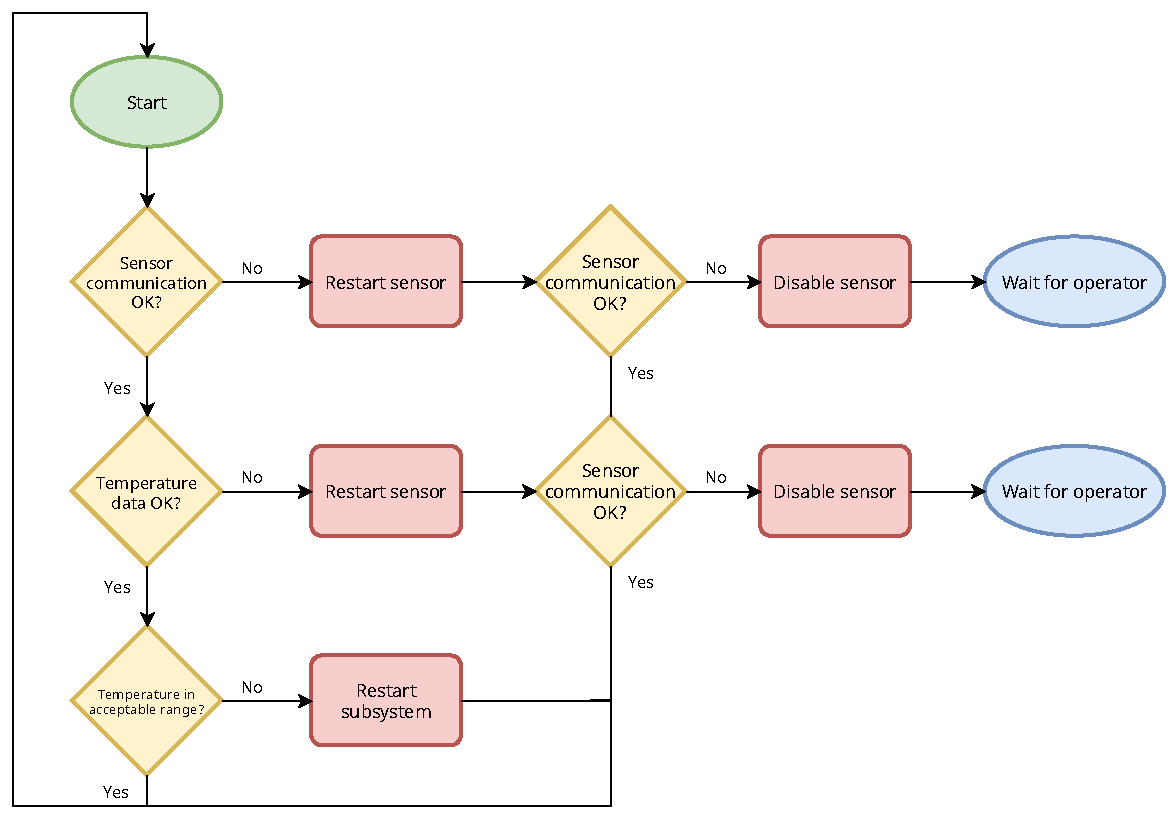
\includegraphics{TempSensorFDIR}
	\caption[Overview of the temperature sensor FDIR process]{Overview of the temperature sensor \ac{FDIR} process. For every process executed and failure detected, corresponding telemetry is generated as well.}
	\label{fig:fdirtemp}
\end{figure*}

The \ac{FDIR} of the sensors follows the hierarchical process described in \Cref{sec:fdir_operating_modes}, which is shown in \Cref{fig:fdirtemp} as tailored for the sensors.

The approach acts using the following steps, which are constantly being executed in the background:
\marginnote[2cm]{For this demonstration, we will not investigate failures of the microcontroller itself and its internals. Refer to \parencite{retselis_acubesat_fmea_2020} for AcubeSAT's \acs{FMEA} and \acs{HSIA} on the microcontrollers.}
\begin{enumerate}
	\item The \ac{I2C} bus health status is monitored. Any failure or lack of communication indicates a failure in the sensor's electronics.
	\item The temperature output of the sensors is monitored. Any values which are outside the bounds of the physically possible thermal conditions are considered to indicate sensor or communication failures. Any values outside the operational limits of the subsystem's electronics are considered to indicate overheating and lead to a subsystem restart.
	\item In order to recover from the failures, first a restart of the sensor is attempted. If the erroneous values still persist, then the sensor cannot recover from the failure, but is just isolated and disabled instead.
\end{enumerate}

\begin{margintable}
	\begin{tabularx}{\linewidth}{@{}rX@{}}
		\toprule
		Severity Category & Level\\ \midrule
		Catastrophic & 1 \\
		Critical & 2 \\
		Major & 3 \\
		Minor/Negligible & 4 \\ \bottomrule
	\end{tabularx}
	\caption{Severity level assignment of \Cref{tab:fmea}}
\end{margintable}

\clearpage
\paragraph{\acl{HSIA}}

After defining the possible failure modes and logic of the system, we are ready to analyse each entry to provide the correct software inputs to implement the required \ac{FDIR}. More specifically, for each failure, the following must be defined \autocite[84]{SAVOIR-HB-003}:
\begin{compactitem}
	\item Parameters to be monitored for detection
	\item Value ranges to be used to warn that a parameter is exceeding a specified range
	\item Isolation and reconfiguration actions to prevent failure propagation and, if possible, bring the system to a well operating state
\end{compactitem}

The above information is listed in the \textbf{\acf{HSIA}} table, which links each failure (identified in the \acl{FMEA}) to the corresponding low-level software parameters (\Cref{tab:hsia}).

For the purposes of this demonstration, we will consider that all \ac{FMEA} items can lead to \emph{feared events}, i.e. that \ac{FDIR} will anticipate all identified possible failures.

\begin{table*}
	\centering
	\caption{HSIA table}
	\label{tab:hsia}
	\begin{tabular}{@{}lL{4cm}L{4cm}L{1cm}L{1cm}L{3.5cm}@{}}
		\toprule
		ID & Failure Mode & Monitored Parameters & Monitoring ID & Event ID & Failure Recovery Action \\ \midrule
		\multicolumn{6}{l}{Temperature sensor MCP9808 \#1} \\ \midrule
		
		
		
		\textbf{\texttt{F-010}} & Temporary loss of function & \(\texttt{T1\_Status} = \texttt{TIMEOUT}\) \newline for 2 times & 0 & 0 & Power-cycle sensor 1 \\
		\textbf{\texttt{F-020}} & Permanent loss of function & \(\texttt{T1\_Status} = \texttt{TIMEOUT}\) \newline for 5 times & 2 & 2 & Ignore sensor 1 values \\
		\textbf{\texttt{F-030}} & Short Circuit between power pins & \(\texttt{T1\_Status} = \texttt{TIMEOUT}\) \newline for 5 times & 2 & 2 & Ignore sensor 1 values \\[5ex]
		\textbf{\texttt{F-040}} & Temporary Value Shift & 
		\(
		\begin{cases}
		\left|\Delta T\right| & > \SI{5}{\celsius} \text{ or} \\
		T_1 &> \SI{100}{\celsius} \text{ or} \\
		T_1 &< \SI{-40}{\celsius}
		\end{cases}
		\) \newline for 2 times
		& 4, 6 & 0, 4 & Power-cycle sensor 1 \\
		\textbf{\texttt{F-050}} & Permanent Value Shift & \(
		\begin{cases}
		\left|\Delta T\right| & > \SI{5}{\celsius} \text{ or} \\
		T_1 &> \SI{100}{\celsius} \text{ or} \\
		T_1 &< \SI{-40}{\celsius}
		\end{cases}
		\) \newline for 5 times & 7, 9 & 2, 5 & Ignore sensor 1 values \\[9ex]
		\textbf{\texttt{F-060}} & \acs{I2C} bus pin output stuck & \(\texttt{T1\_Status} = \texttt{TIMEOUT}\) \newline for 5 times & 2 & 2 & Ignore sensor 1 values \\ \midrule
		
		
		
		\multicolumn{6}{l}{Temperature sensor MCP9808 \#2} \\ \midrule
		
		
		
		\textbf{\texttt{F-070}} & Temporary loss of function & \(\texttt{T2\_Status} = \texttt{TIMEOUT}\) \newline for 2 times & 1 & 1 & Power-cycle sensor 2 \\
		\textbf{\texttt{F-080}} & Permanent loss of function & \(\texttt{T2\_Status} = \texttt{TIMEOUT}\) \newline for 5 times & 3 & 3 & Ignore sensor 2 values \\
		\textbf{\texttt{F-090}} & Short Circuit between power pins & \(\texttt{T2\_Status} = \texttt{TIMEOUT}\) \newline for 5 times & 3 & 3 & Ignore sensor 2 values \\[5ex]
		\textbf{\texttt{F-100}} & Temporary Value Shift & 
		\(
		\begin{cases}
		\left|\Delta T\right| & > \SI{5}{\celsius} \text{ or} \\
		T_2 &> \SI{100}{\celsius} \text{ or} \\
		T_2 &< \SI{-40}{\celsius}
		\end{cases}
		\) \newline for 2 times
		& 5, 6 & 1, 4 & Power-cycle sensor 2 \\
		\textbf{\texttt{F-110}} & Permanent Value Shift & \(
		\begin{cases}
		\left|\Delta T\right| & > \SI{5}{\celsius} \text{ or} \\
		T_2 &> \SI{100}{\celsius} \text{ or} \\
		T_2 &< \SI{-40}{\celsius}
		\end{cases}
		\) \newline for 5 times & 8, 9 & 3, 5 & Ignore sensor 2 values \\[9ex]
		\textbf{\texttt{F-120}} & \acs{I2C} bus pin output stuck & \(\texttt{T2\_Status} = \texttt{TIMEOUT}\) \newline for 5 times & 3 & 3 & Ignore sensor 2 values \\ \midrule
		
		
		
		\multicolumn{6}{l}{Subsystem} \\ \midrule
		
		
		
		\textbf{\texttt{F-130}} & Overheating & \(T_1 > \SI{50}{\celsius}\) or \(T_2 > \SI{50}{\celsius}\) & 10, 11 & 6 & Restart subsystem \\ \bottomrule
	\end{tabular}
	\vspace{2pt}
\end{table*}

The \ac{HSIA} adds the following significant pieces of information to the \ac{FMEA} \autocite{ECSS-Q-ST-30-02C}:
\begin{itemize}
	\item The \textbf{monitored parameters} and the \textbf{conditions} that trigger the recovery action.
	
	These are listed here in terms of \ac{PUS} parameters which can be easily identified and compared by software. This list is then linked to the corresponding \emph{\texttt{ST[12]} on-board monitoring} service definitions, listed in \Cref{tab:demo_monitoring}.
	
	It is important to note that no single out-of-bounds value can trigger a recovery action. This is recommended in order to prevent transient errors or temporary communication protocol issues from triggering an unnecessary response which might disable a well-functioning component.
	
%	\marginnote{\textbf{Temporary failure}: Caused by events such as bit flips, noise or transients, and can be corrected without intervention, or with a simple restart/power-cycle.\par\textbf{Permament failure}: A failure (typically in hardware, e.g.\ due to latchups or short-circuits) that cannot be corrected autonomously.}
	The distinction between \emph{temporary} and \emph{permanent} failures is made by \textbf{counting the number of consecutive failures}. Before a permanent action to disable a sensor is enacted, at least 5 attempts to communicate must have failed.
	
	The use of dual hot-redundant sensors also allows us to investigate the difference between the two temperatures to deduce the health of the produced data. If the absolute difference between the 2 values is too high, assuming the sensors are placed close enough together, an error condition is assumed. However, as triple modular redundancy was not implemented for this system, it is not possible to deduce which sensor has failed.
	
	Note that for this demonstration, we chose thresholds and timings that may slightly differ from the actual mission thresholds and limits, in order to ease testing and results presentation.
	
	\item The \textbf{failure recovery and isolation actions}.
	
	These are listed in terms of \ac{PUS} events (\emph{\texttt{ST[05]} event reporting}) and event-actions (\emph{\texttt{ST[19]} eventaction}), which are linked to \Cref{tab:demo_eventaction}.
	
	The selected recovery actions match the approach shown in \Cref{fig:fdirtemp}. Additionally, when it is not known which sensor has failed, a fail-safe approach of restarting or disabling both sensors is used.
\end{itemize}

\paragraph{Parameters}

After investigating the \acl{HSIA}, we can list the scalar parameters for the \emph{\texttt{ST[20]} parameter management} service (\Cref{tab:demo_params}).

Beyond the actual temperature values, we have included the \textbf{difference} (\(\Delta\)) between the two temperatures, since the \acs{PUS} standard does not provide ways to perform arithmetic calculations without hard-coded software. Additionally, the status of each sensor peripheral is included, which is an enumerated value.\footnote{One of \texttt{NOMINAL}, \texttt{TIMEOUT} or \texttt{DISABLED}} 

These parameters are telemetered to the ground segment and displayed to the user periodically, via the \emph{\texttt{ST[03]} housekeeping} \ac{PUS} service. However, during flight, the ground segment will not have constant access, since the satellite will not be visible from ground stations throughout its entire orbit.

\begin{table}[h]
	\centering
	\caption[List of \texttt{ST[20]} parameters]{List of \texttt{ST[20]} parameters\\R: Read-only\\RW: Read-write}
	\label{tab:demo_params}
	\begin{tabularx}{\textwidth}{@{}rlllX@{}}
		\toprule
		Param. ID & Parameter              & Units & Type & Type \\ \midrule
		0            & Temperature 1          & \si{\celsius}      & \texttt{float} & R     \\
		1            & Temperature 2          & \si{\celsius}      & \texttt{float} & R    \\
		2            & \(\Delta\) Temperature & \si{\celsius}      & \texttt{float} & R    \\
		3            & Temperature 1 Status         &       & Enumerated   & RW  \\
		4            & Temperature 2 Status         &       & Enumerated   & RW  \\
		5			 & Temperature 1+2 Status       &		& Enumerated   & R  \\ \bottomrule
	\end{tabularx}
	\vspace{.5em}
\end{table}

\paragraph{On-board monitoring definitions}

After defining the parameters, the monitoring definitions that establish the acceptable and actionable ranges for each parameter should be outlined. These are then managed by the \emph{\texttt{ST[12]} on-board monitoring} \ac{PUS} service.

The \emph{check validity conditions} are important to mention in this case, as they use the three \emph{Status} parameters to prevent executing checks for disabled peripherals. As such, sensors that are not providing values due to hardware issues, \ac{FDIR} actions or operator intervention, will not be able to trigger \ac{FDIR} actions.

\begin{table*}[h]
	\centering
	\caption[List of \texttt{ST[12]} monitoring definitions][5pt]{List of \texttt{ST[12]} monitoring definitions. \(t\) and \(\Delta\) are used as placeholders for parameter values.}
	\label{tab:demo_monitoring}
	\begin{adjustbox}{width=\textwidth}
	\begin{tabular}{@{}L{1cm}L{2.5cm}L{2.8cm}L{2cm}L{2cm}L{2cm}ll@{}}
		\toprule
		&  & \multicolumn{2}{c}{Check validity condition} &  &  & \multicolumn{2}{c}{Check} \\ \cmidrule(lr){3-4} \cmidrule(l){7-8} 
		Definition ID & Monitored Parameter & Validity Parameter & Expected Value & Monitoring Interval & Repetition Number & Check Type & Criteria \\ \midrule
		0 & Temp. 1 Status &  &  & \SI{500}{\milli\second} & 2 & Expected Value & \(\neq\) \texttt{TIMEOUT} \\
		1 & Temp. 2 Status &  &  & \SI{500}{\milli\second} & 2 & Expected Value & \(\neq\) \texttt{TIMEOUT} \\
		2 & Temp. 1 Status &  &  & \SI{500}{\milli\second} & 5 & Expected Value & \(\neq\) \texttt{TIMEOUT} \\
		3 & Temp. 2 Status &  &  & \SI{500}{\milli\second} & 5 & Expected Value & \(\neq\) \texttt{TIMEOUT} \\
		\midrule
		4 & Temperature 1 & Temp. 1 Status & \texttt{NOMINAL} & \SI{500}{\milli\second} & 2 & Range & \( -\SI{40}{\celsius} < t < \SI{100}{\celsius} \) \\
		5 & Temperature 2 & Temp. 2 Status & \texttt{NOMINAL} & \SI{500}{\milli\second} & 2 & Range & \( -\SI{40}{\celsius} < t < \SI{100}{\celsius} \) \\
		6 & \(\Delta\) Temperature & Temp. 1+2 Status & \texttt{NOMINAL} & \SI{500}{\milli\second} & 2 & Range & \( -\SI{5}{\celsius} < \Delta < \SI{5}{\celsius} \) \\
		\midrule
		7 & Temperature 1 & Temp. 1 Status & \texttt{NOMINAL} & \SI{500}{\milli\second} & 5 & Range & \( -\SI{40}{\celsius} < t < \SI{100}{\celsius} \) \\
		8 & Temperature 2 & Temp. 2 Status & \texttt{NOMINAL} & \SI{500}{\milli\second} & 5 & Range & \( -\SI{40}{\celsius} < t < \SI{100}{\celsius} \) \\
		9 & \(\Delta\) Temperature & Temp. 1+2 Status & \texttt{NOMINAL} & \SI{500}{\milli\second} & 5 & Range & \( -\SI{5}{\celsius} < \Delta < \SI{5}{\celsius} \) \\
		\midrule
		10 & Temperature 1 & Temp. 1 Status & \texttt{NOMINAL} & \SI{500}{\milli\second} & 5 & Range & \( t < \SI{50}{\celsius} \) \\
		11 & Temperature 2 & Temp. 2 Status & \texttt{NOMINAL} & \SI{500}{\milli\second} & 5 & Range & \( t < \SI{50}{\celsius} \) \\ \bottomrule
	\end{tabular}
	\end{adjustbox}
	\vspace{.5em}
\end{table*}

\paragraph{Event-action definitions}

The final part of the puzzle are the event-action definitions, which can be seen on \Cref{tab:demo_eventaction} and combine:
\begin{itemize}
	\item \ac{PUS} events (\texttt{ST[05]} service) which are automatically generated when an on-board monitoring definition goes out of limits.
	\item \ac{PUS} event-action definitions (\texttt{ST[19]} service), which link every occurrence of an event to a stored \ac{TC} that is immediately executed.
	They define the \acs{FDIR} recovery actions.
\end{itemize}

All the aforementioned definitions can be easily modified by operators using single commands that affect the on-board stored \ac{PUS} database.

\begin{table}[h]
	\centering
	\caption{List of \texttt{ST[19]} event-action definitions}
	\label{tab:demo_eventaction}
	\begin{tabular}{@{}lL{2cm}L{7cm}@{}}
		\toprule
		Event ID & Monitoring Definitions & Action \\ \midrule
		0 & 0, 4 & Restart sensor 1 \\
		1 & 1, 5 & Restart sensor 2 \\
		2 & 2, 7 & Set sensor 1 status \( = \) \texttt{DISABLED} \\
		3 & 3, 8 & Set sensor 2 status \( = \) \texttt{DISABLED} \\
		4 & 6 & Restart all sensors \\
		5 & 9 & Set all sensors status \( = \) \texttt{DISABLED} \\
		6 & 10, 11 & Restart system \\ \bottomrule
	\end{tabular}
\end{table}

\clearpage
\section{\ac{FDIR} validation}

In this section, we present the verification and validation actions of the \acs{FDIR} system, so we can conclude whether the given requirements are covered, and if the system can correct all failures as requested.

\subsection{Nominal operation}

During nominal operation, no failures are simulated. The system is connected to power and outputs \ac{ECSS} telemetry (\Cref{fig:yamcshousekeeping}), which includes parameter values parsed by (\Cref{fig:yamcsparameter}). Additionally, a log file is kept for diagnostic purposes (\Cref{fig:lognominal}). The system is compliant with its requirements (\Cref{sec:tsvcd}) and can transmit the temperature to the ground station as expected.

\begin{figure}
	\centering
	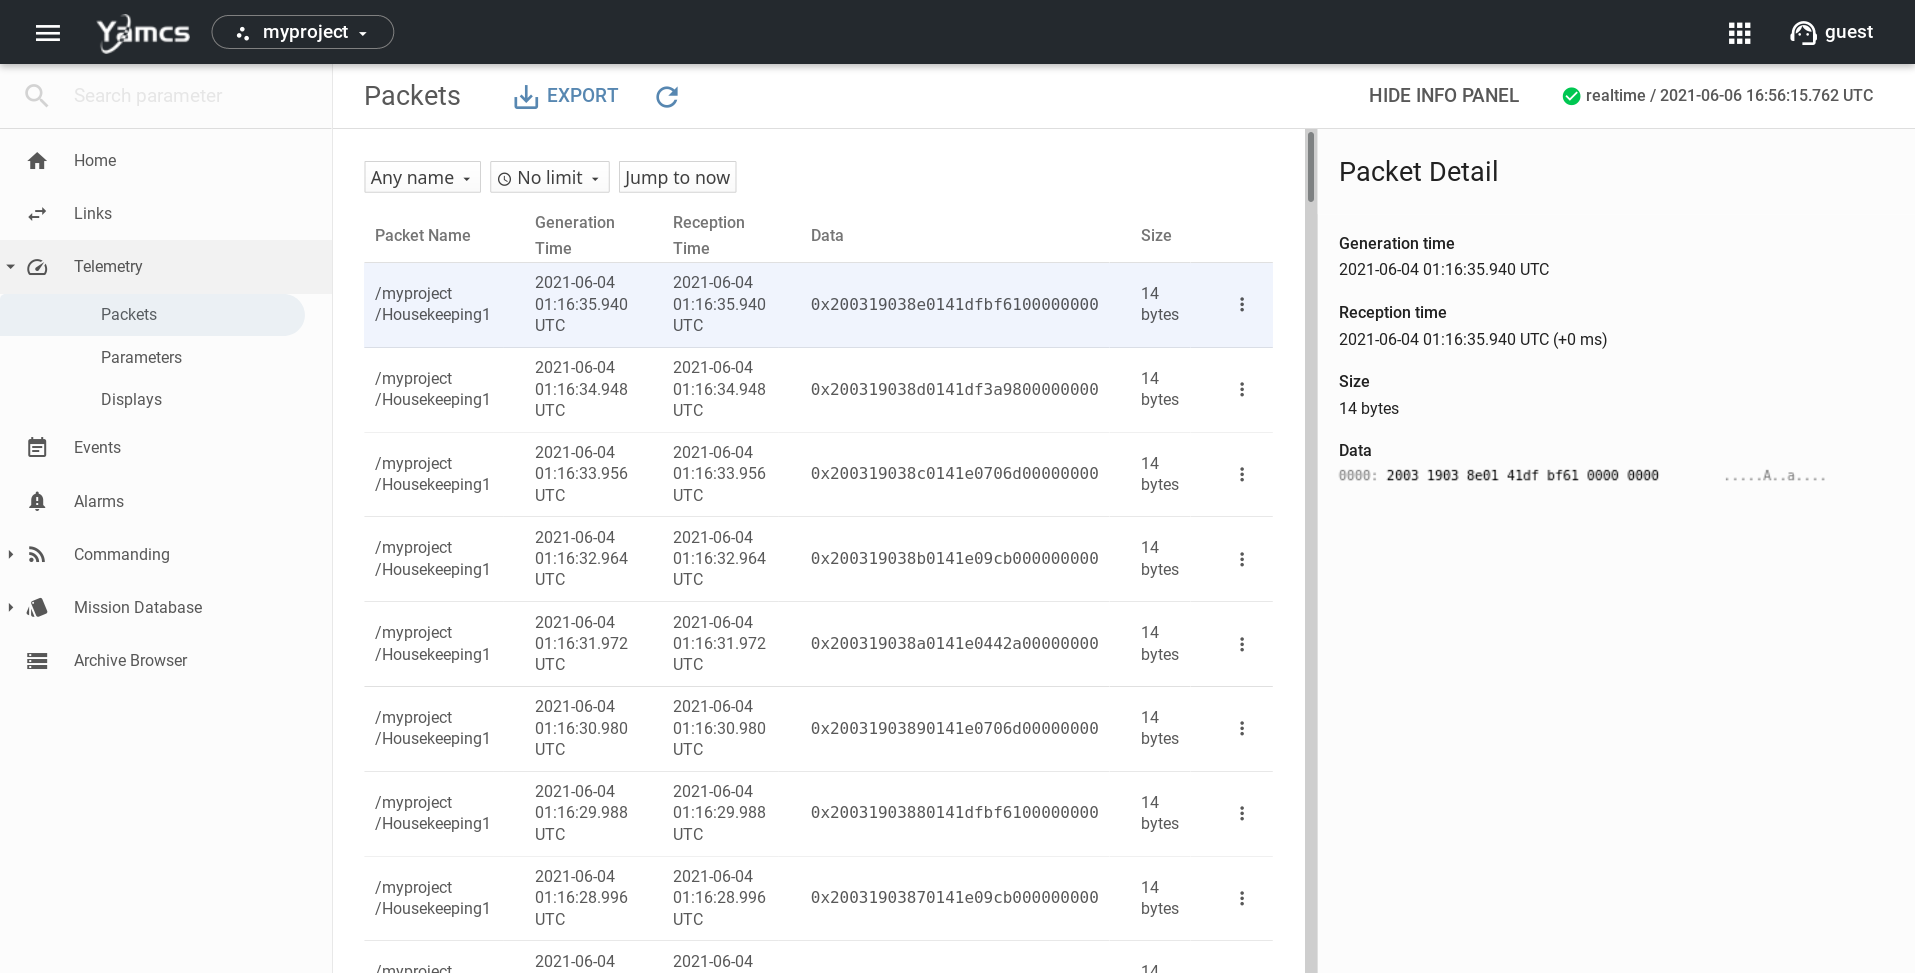
\includegraphics{media/screenshots/yamcs_housekeeping}
	\caption{View of housekeeping packets generated by the \acs{MCU} in \acs{YAMCS}}
	\label{fig:yamcshousekeeping}
\end{figure}

\begin{figure}[h]
	\centering
	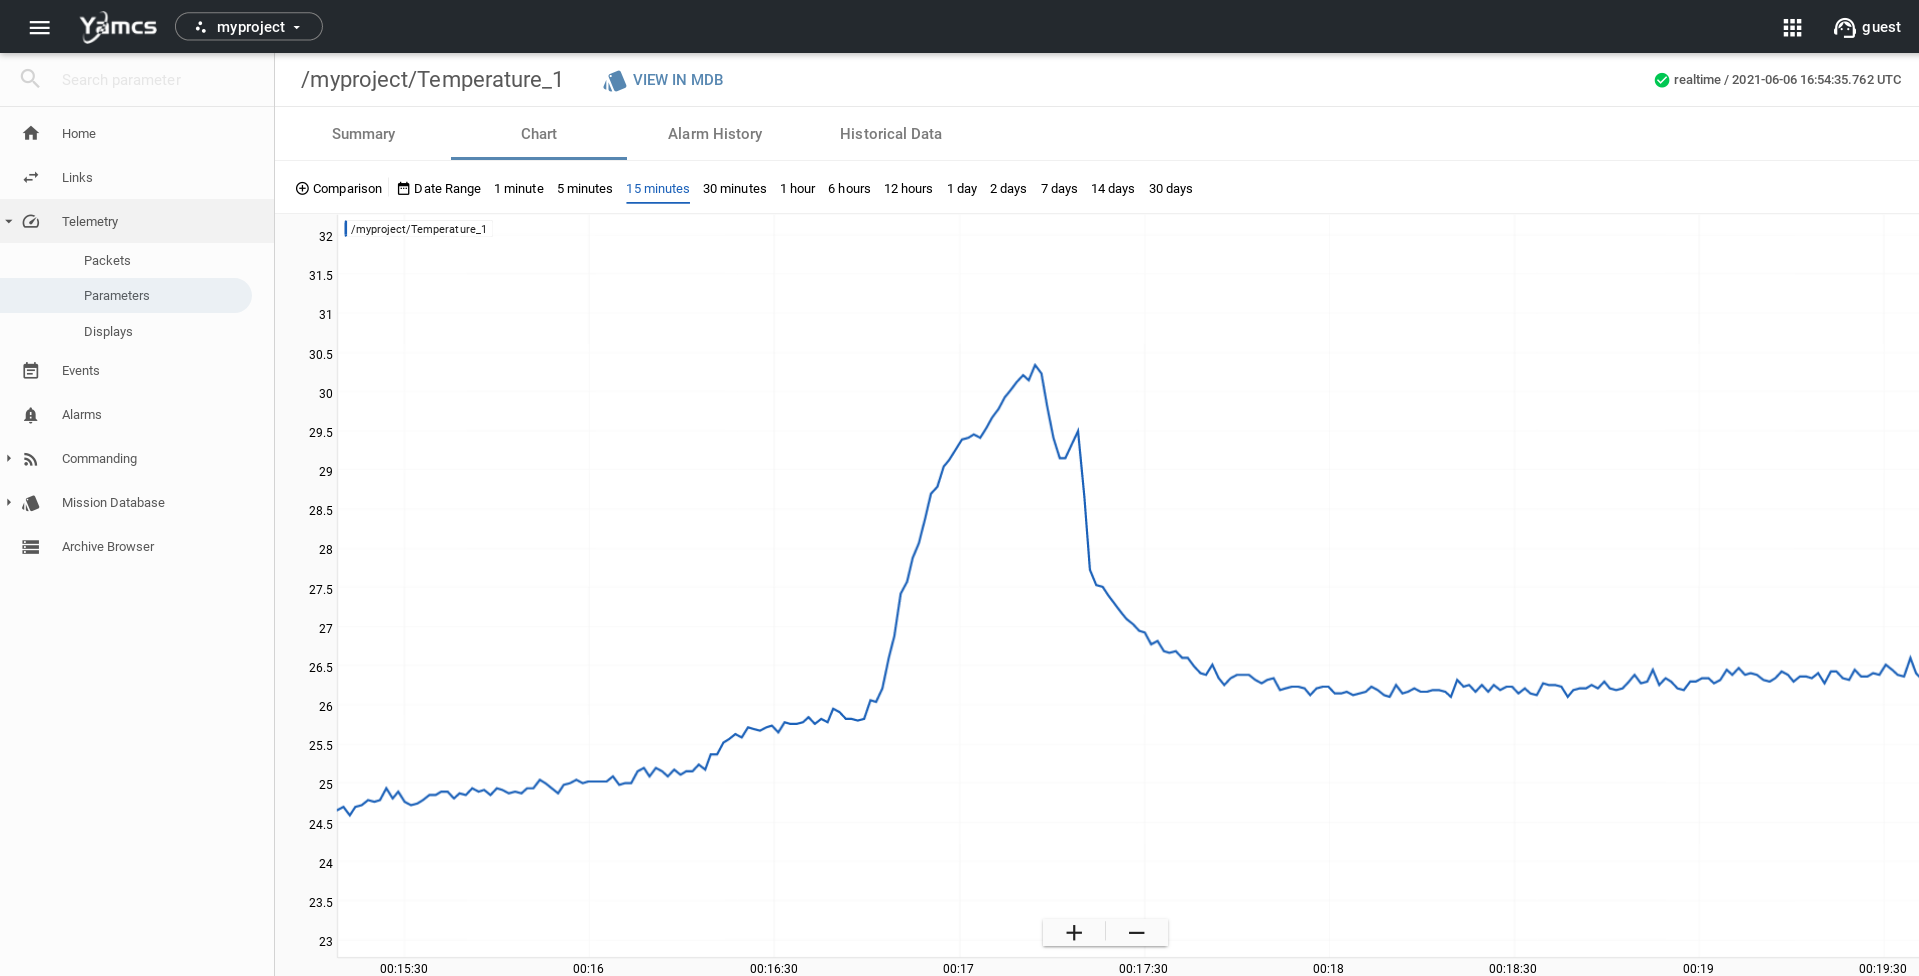
\includegraphics{media/screenshots/yamcs_parameter}
	\caption{View of one temperature parameter in \acs{YAMCS}}
	\label{fig:yamcsparameter}
\end{figure}

\begin{figure}
\begin{cminted}{text}
909601  [debug  ] T1 = 28.18
909701  [debug  ] T1 = 28.08
909801  [debug  ] T1 = 28.14
909901  [debug  ] T1 = 27.97
910000  [trace  ] New TM [3,25]
910001  [debug  ] T1 = 28.10
910101  [debug  ] T1 = 28.03
910201  [debug  ] T1 = 28.12
910301  [debug  ] T1 = 27.90
910401  [debug  ] T1 = 28.08
\end{cminted}
\caption[Log output during nominal operation]{Log output during nominal operation. The first number is the \ac{MCU} tick counter in milliseconds since boot.}
\label{fig:lognominal}
\end{figure}

\marginnote{
Monitoring status types \autocite{ECSS-E-ST-70-41C}:

\begin{compactitem}[{}]
	\item[\unchecked:] This check is disabled
	\item[\ok:] The parameter is within limits
	\item[\invalid:] The \emph{check validity condition} is \texttt{false}. This check is not performed.
	\item[\textcolor{unexpected}{Any other}:] Parameter is out of limits
\end{compactitem}
}

It is of particular interest to examine the state of the \acs{FDIR} system during microcontroller startup. The first \acs{ECSS} data we see is shown in \Cref{fig:pus_boot}. The image shows the \textbf{transitions} of the \emph{\texttt{ST[12]} on-board monitoring} service, as shown in the interface we developed (\Cref{sec:pusinterface}). In practice, this view shows the \textbf{outcome} of each check, and if the value is within bounds, out of bounds, or if the check is disabled.

\begin{figure}
	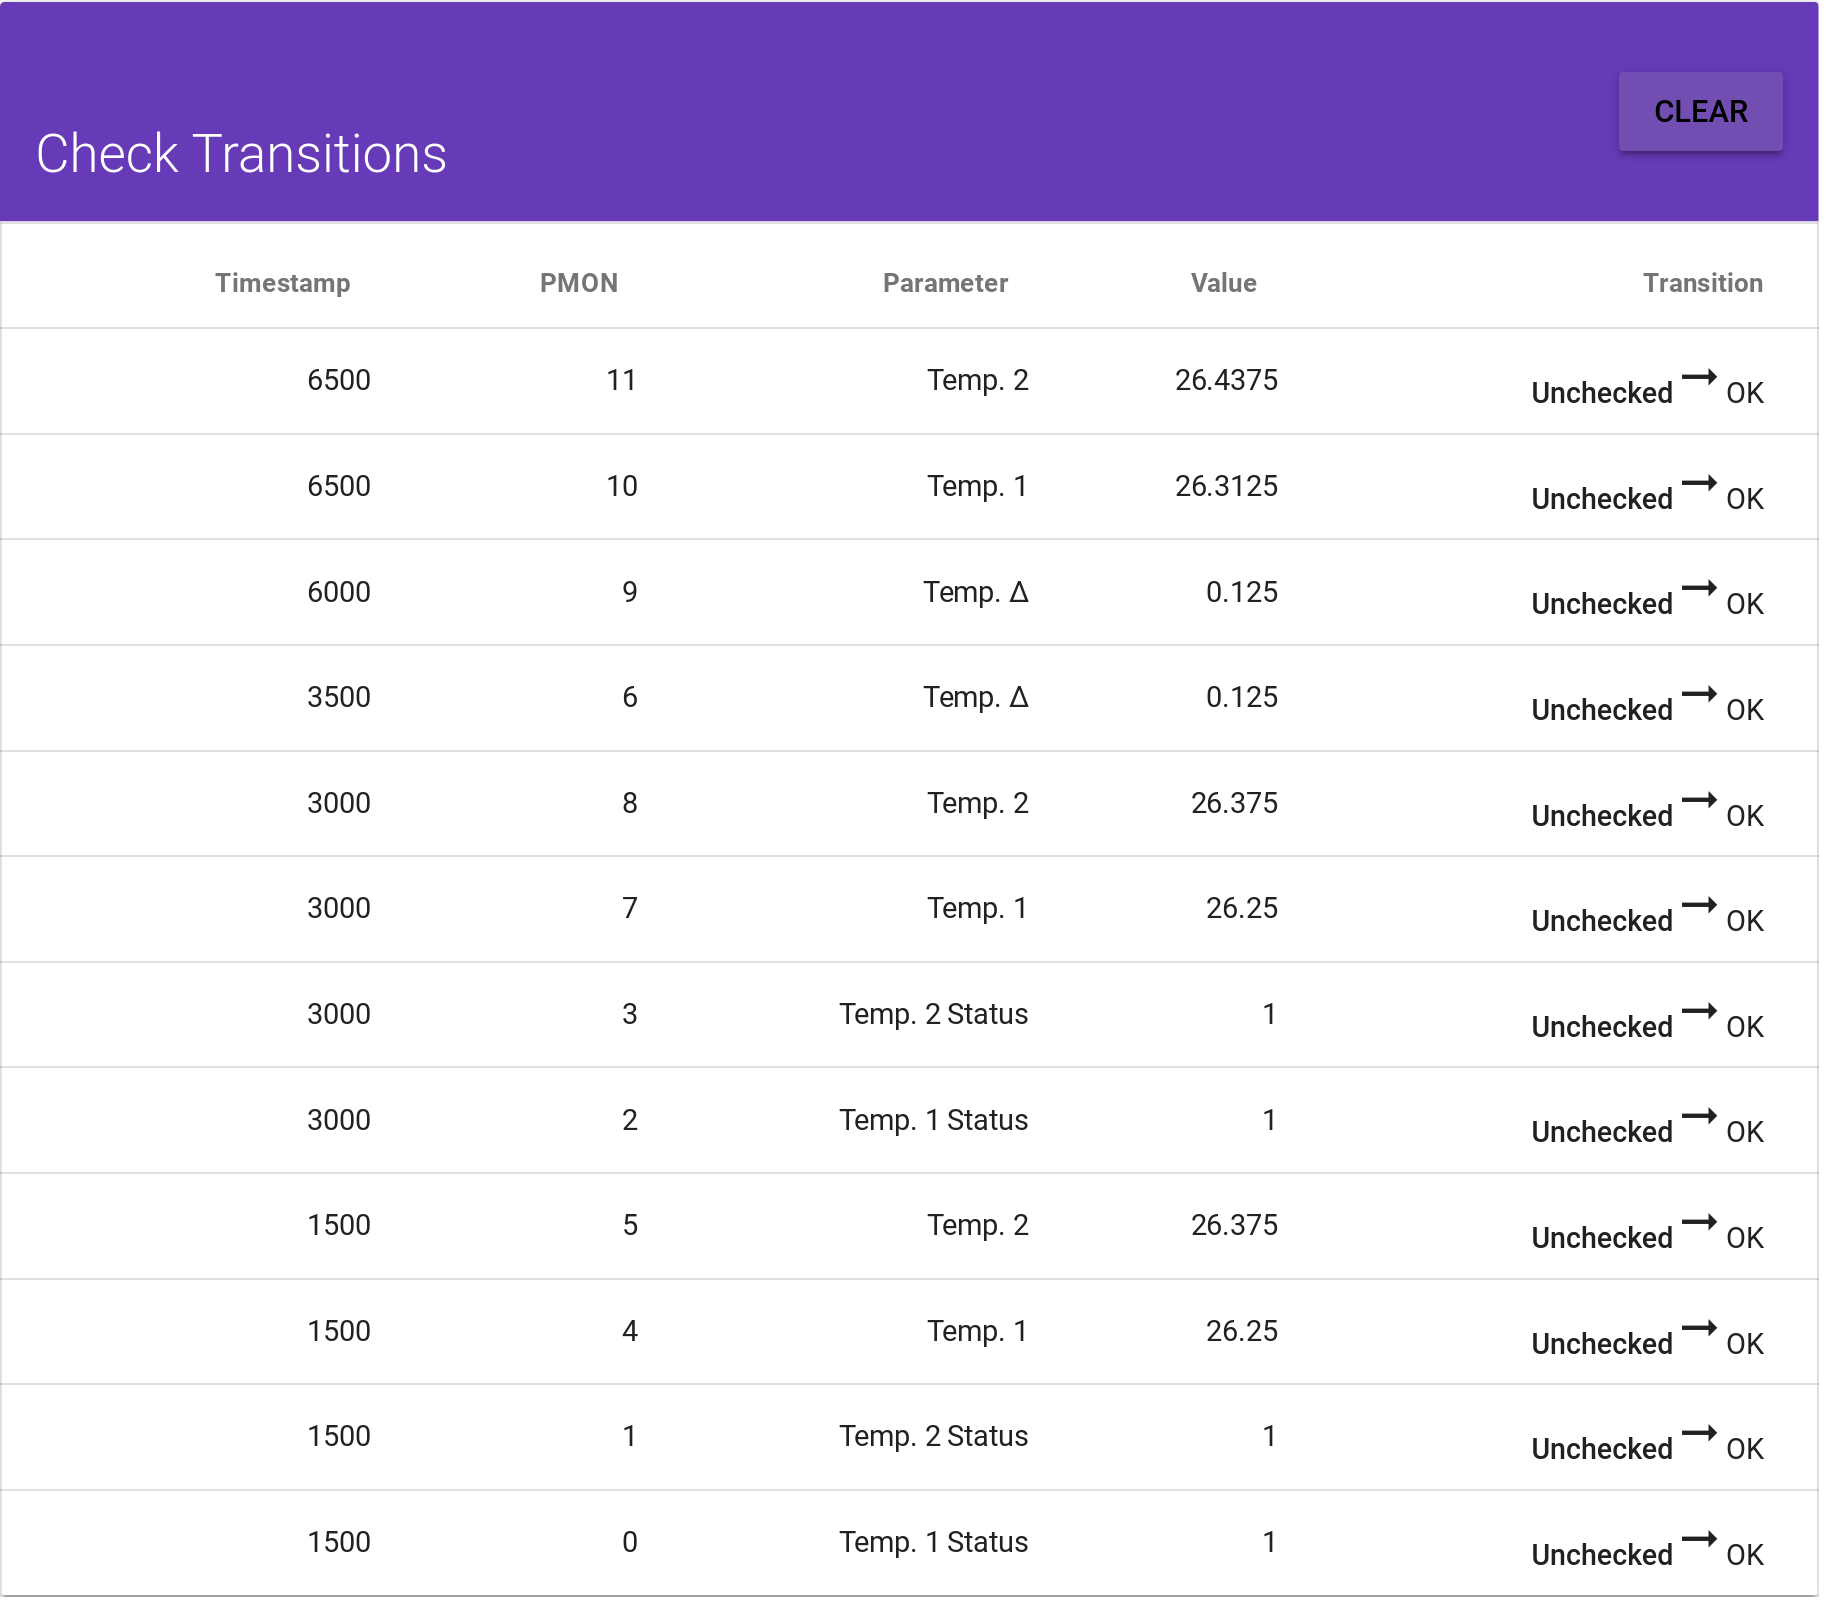
\includegraphics{screenshots/pus_boot}
	\caption{Transitions made at boot}
	\label{fig:pus_boot}
\end{figure}

In this example, we can observe that all 12 checks transition from the \unchecked{} state to the \ok{} state. This happens because, upon system startup, all monitoring definitions are in the initial state \unchecked, indicating that they have never been executed. After the repetition count \emph{times} the monitoring period of each definition has passed, the variable is considered to have a value within bounds, and the definition is \ok.

The different transition time of each definition is attributed to the different \textbf{repetition count} of the definitions. To register the transition, the parameter must have been measured as many times as the repetition count.

As long as the transitions lead to a state within bounds, no other report is generated, nor any other repair mechanism is triggered. The system works correctly.

\begin{figure}[h]
	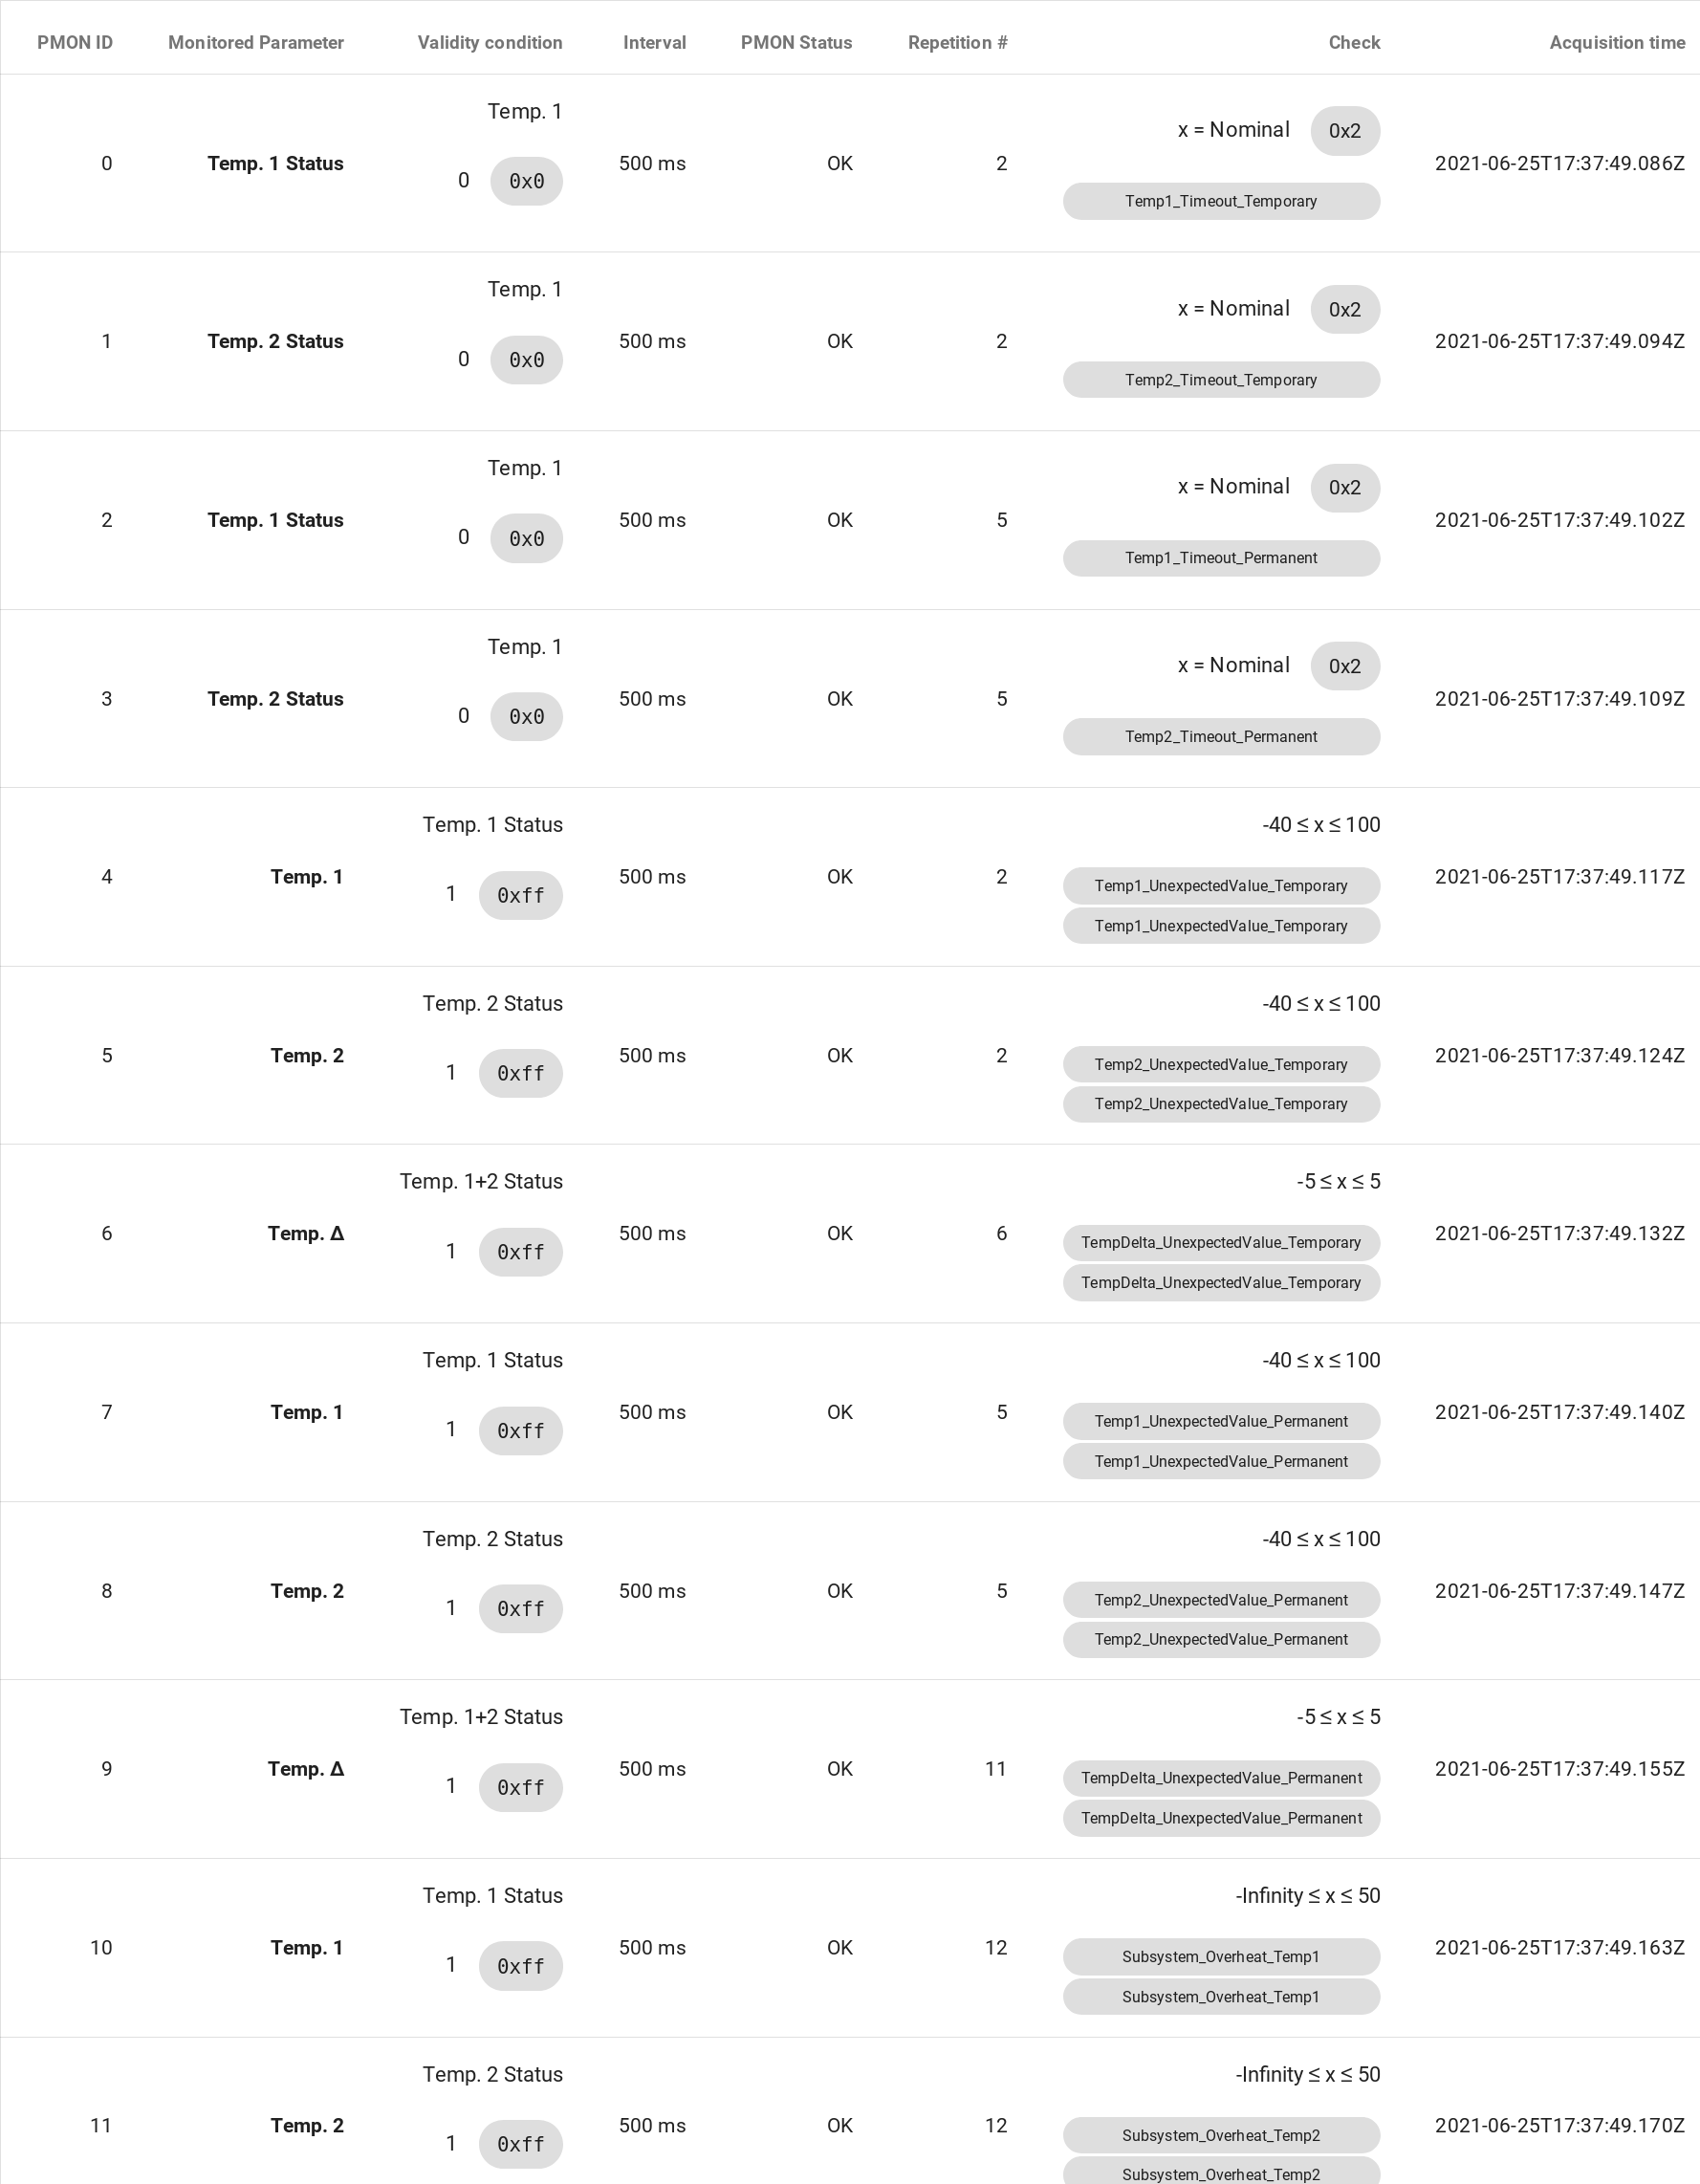
\includegraphics{screenshots/pus_obmd}
	\caption[List of monitoring definitions at startup, without failures]{List of monitoring definitions at startup, without failures. This data is obtained as \acs{TM} from the \acs{MCU} and corresponds exactly to the values of \Cref{tab:demo_monitoring}.}
		\label{fig:pus_obmd}
\end{figure}
	
\begin{figure}[h]
	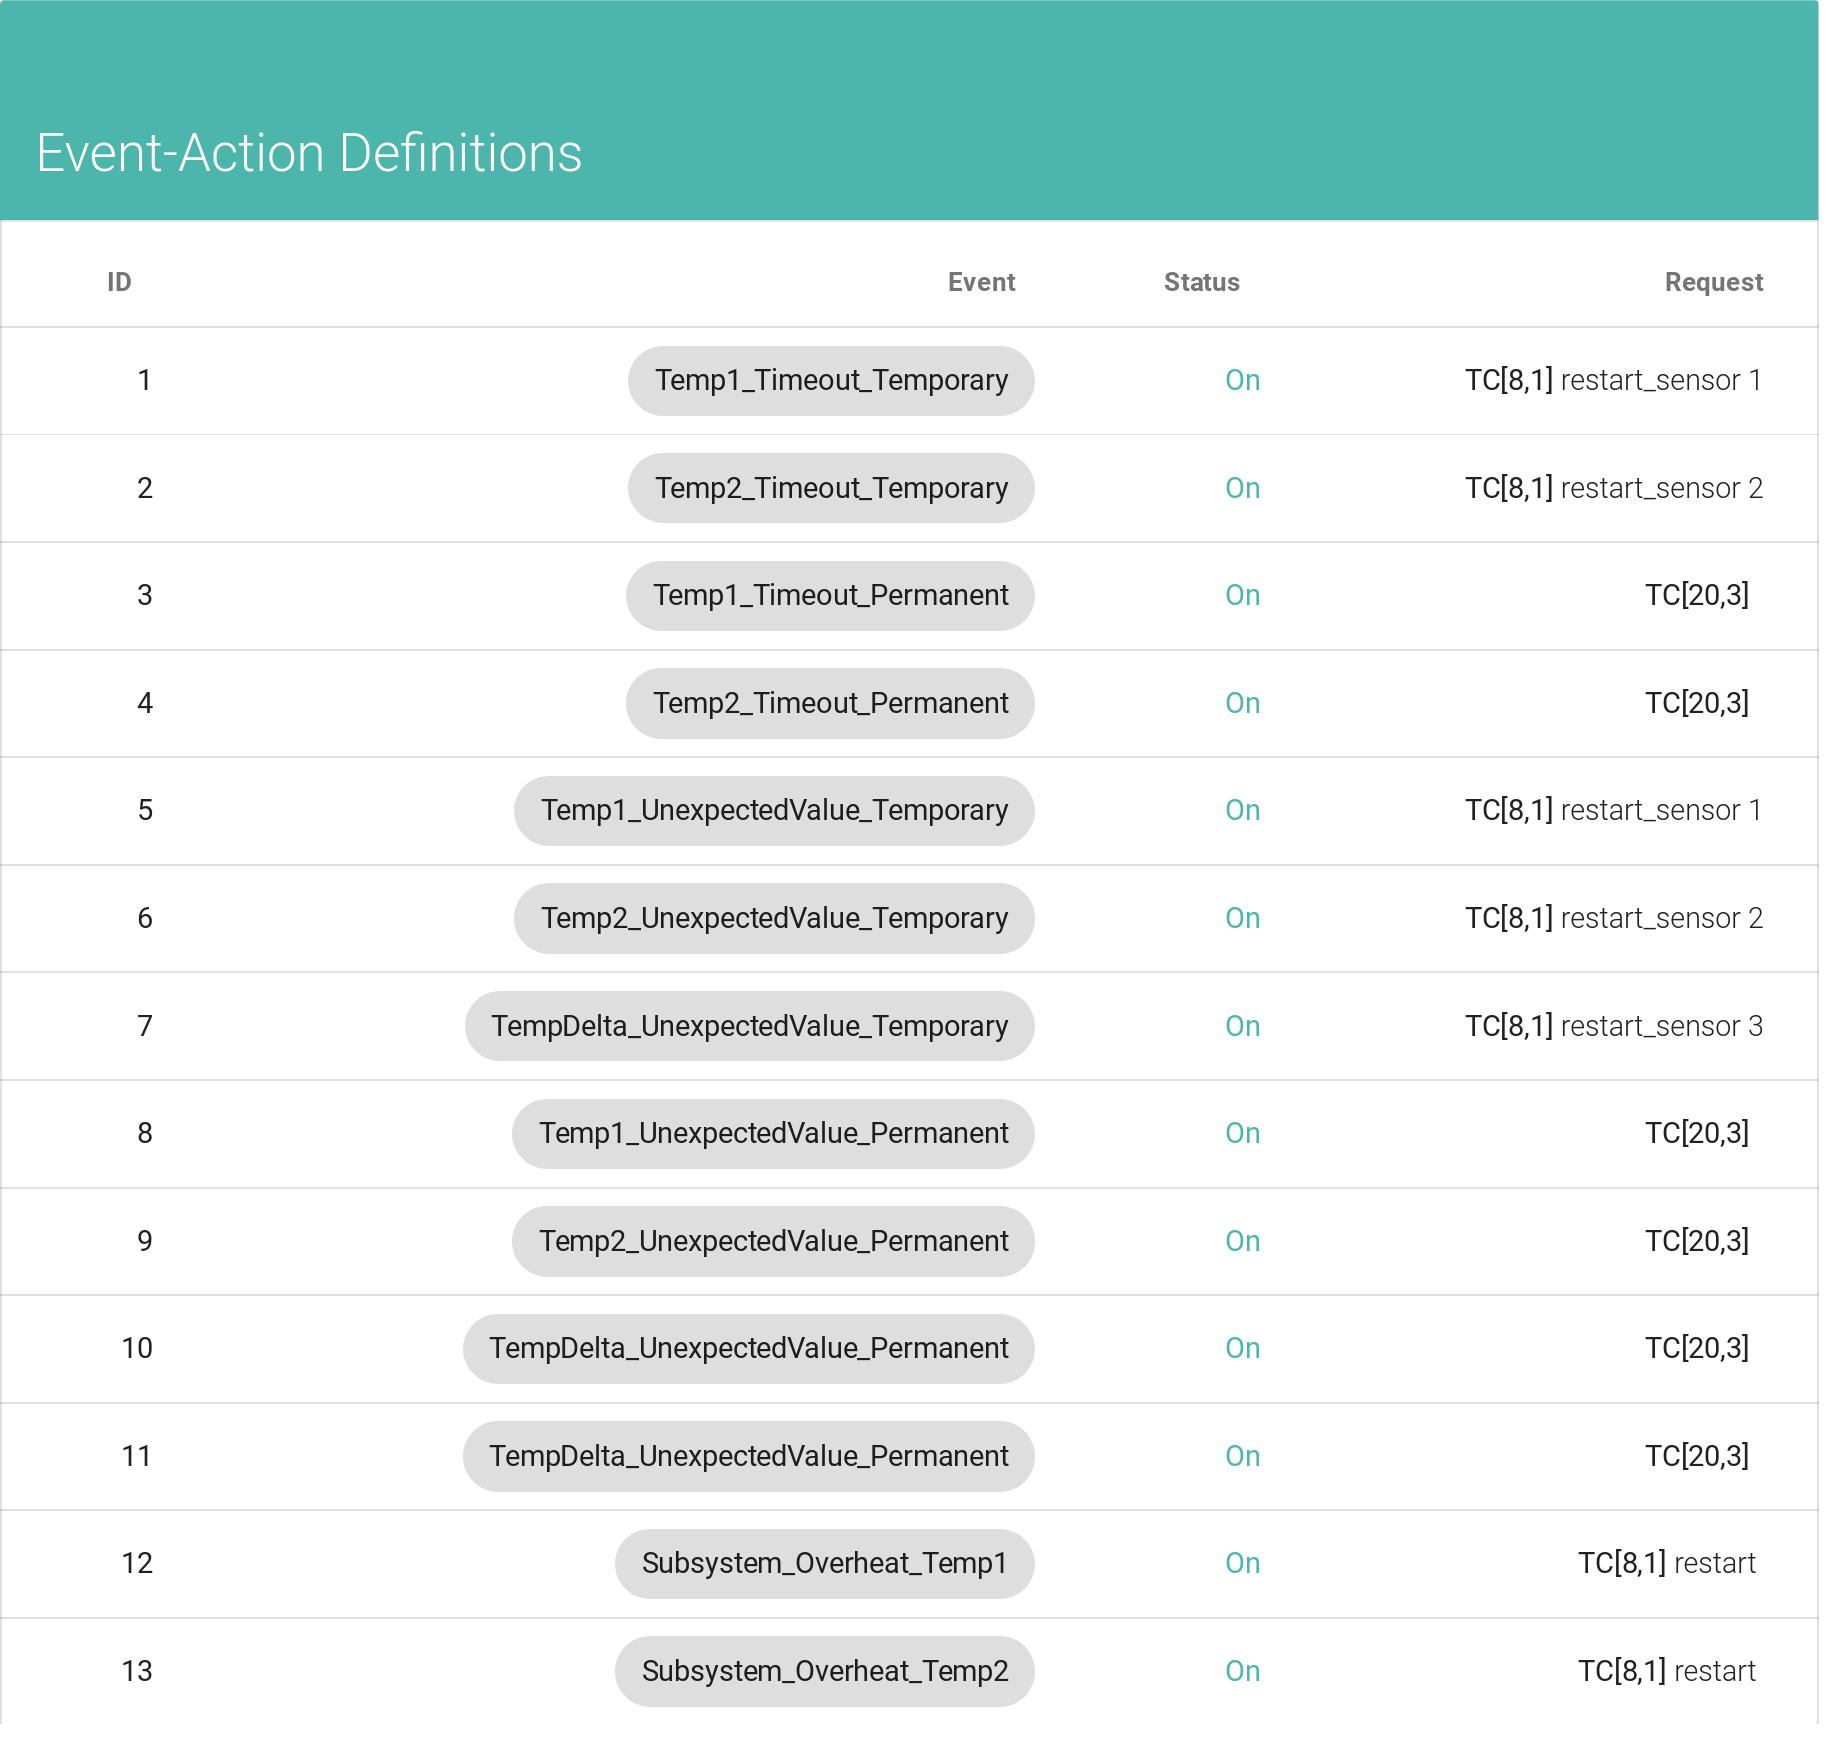
\includegraphics{screenshots/pus_eventaction}
	\caption[List of event-action definitions]{List of event-action definitions at startup, without failures. This data is received as \acs{TM} from the \acs{MCU} and corresponds exactly to the values of \Cref{tab:demo_eventaction}.}
		\label{fig:pus_eventaction}
\end{figure}
		
At startup, an \emph{\texttt{ST[05]} event reporting} event is generated, which announces the microcontroller startup (\Cref{fig:yamcsmcustart}).
			
\begin{figure}[h]
	\centering
	\caption{The microcontroller startup event, shown through \acs{YAMCS}}
	\label{fig:yamcsmcustart}
	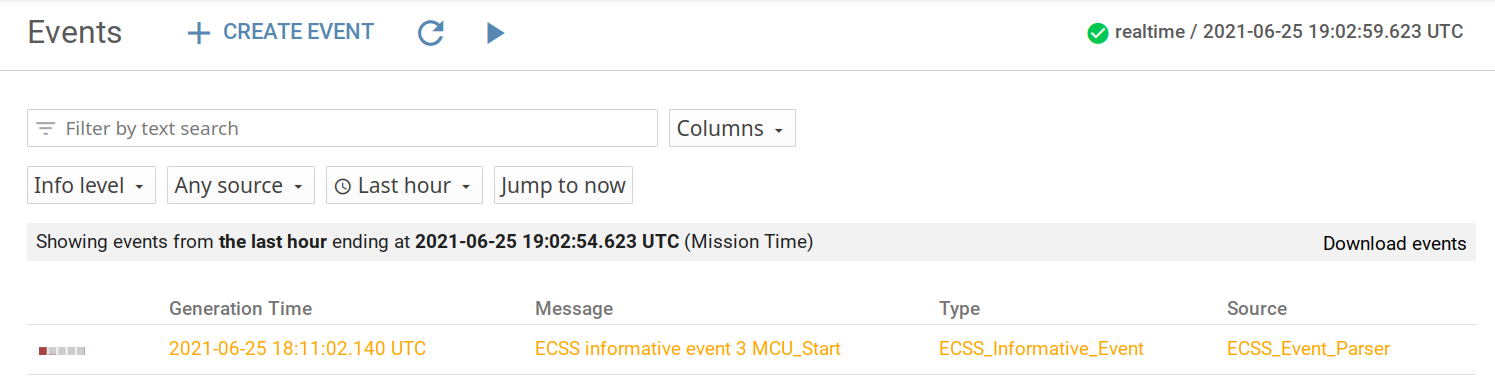
\includegraphics{screenshots/yamcs_mcustart}
\end{figure}

\FloatBarrier
\subsection{Simulation of failures}
\label{sec:simul}

The following methods were used to simulate each failure:
\begin{itemize}
	\item For component communication failures, each sensor was just physically disconnected from the system.
	\item For small changes in temperature, a hot air gun or other hot air source was pointed towards each sensor. Care was taken to not exceed the rated temperatures of the affected components.
	\item For changes in temperature which were impractical to simulate, the failure was injected in software, by manually modifying the variable.
	
	The two buttons present on the development board were used as a simple interface to ``inject'' extreme temperature values.
\end{itemize}

\begin{table*}
	\centering
	\caption{Overview of failure simulation methods}
	\label{tab:testfailures}
	\renewcommand{\arraystretch}{1.5}
	\begin{tabularx}{\textwidth}{@{}lL{4cm}L{3.5cm}X@{}}
		\toprule
		ID & Failure Mode & Recovery action & Simulation method \\ \midrule
		\multicolumn{4}{l}{MCP9808 Temperature Sensor \#1} \\ \midrule
		\textbf{\texttt{F-010}} & Temporary loss of function & Power-cycle sensor 1 & \textbf{Hardware}: Temporary cable disconnection \\
		\textbf{\texttt{F-020}} & Permanent loss of function & Ignore sensor 1 values & \textbf{Hardware}: Permanent cable disconnection \\
		\textbf{\texttt{F-030}} & Short Circuit between pins & Ignore sensor 1 values & \emph{Same as \texttt{F-020}}  \\
		\textbf{\texttt{F-040}} & Temporary Value Shift & Power-cycle sensor 1 & \textbf{Software}: Emulation of large value (temporarily)\newline \textbf{Hardware}: Increase temperature difference (temporarily)\\
		\textbf{\texttt{F-050}} & Permanent Value Shift & Ignore sensor 1 values & \textbf{Software}: Emulation of large value (permanently)\newline\textbf{Hardware}: Increase temperature difference (permanently) \\
		\textbf{\texttt{F-060}} & \acs{I2C} bus pin output stuck & Ignore sensor 1 values & \textbf{Hardware}: Connect \acs{I2C} pin to ground
		\\ \midrule
		\multicolumn{4}{l}{MCP9808 Temperature Sensor \#2} \\ \midrule
		
		\multicolumn{4}{@{}c@{}}{Same as sensor \#1\vspace{1ex}} \\ \midrule
		
		\multicolumn{4}{l}{Subsystem} \\ \midrule
		
		\textbf{\texttt{F-130}} & Overheating  & Subsystem restart & \textbf{Software}: Emulation of large value (temporarily) \\ \bottomrule
	\end{tabularx}
	\vspace{2pt}
\end{table*}

\clearpage
\paragraph{\textbf{\texttt{F-010}: Temporary loss of function (full demo)}}\hspace{0pt}

The first failure we will simulate will be the loss of the \acs{I2C} bus or peripheral. The simulation is done in hardware via \emph{temporary cable disconnection}.

\subparagraph{Procedure}
\begin{compactenum}
	\item Disconnect the \acs{SDA} or \acs{SCL} cable from the breadboard
	\item After 2 seconds, reconnect the cable to reproduce the temporary nature of the failure
\end{compactenum}

\subparagraph{Visual indications} The 1\textsuperscript{st} \acs{LED} light flashes once, and stays on.

\subparagraph{Results}
For this analysis, all the \acs{FDIR} steps and processes will be shown in detail, including the visual information provided to the operators. However, subsequent failure modes will have only an overview presented, centred around the transition tables.

Before studying the failure and \acs{FDIR} results, we will look at the \acs{ECSS} parameters and their values.

\begin{figure}[h]
	\centering
	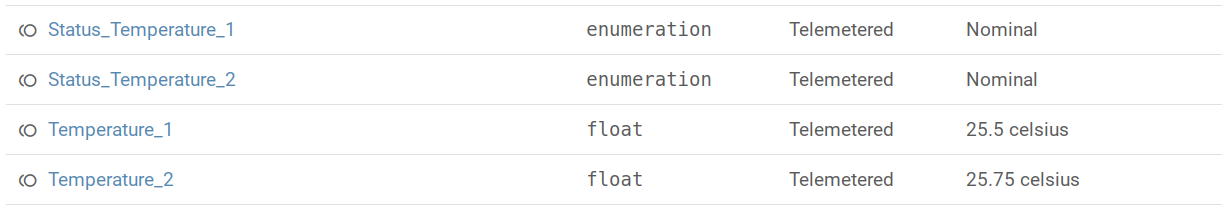
\includegraphics{screenshots/yamcs_parameters}
	\caption{\acs{YAMCS} temperature parameters in nominal operation}
	\label{fig:yamcsparametersnominal}
\end{figure}

\begin{figure}[h]
	\centering
	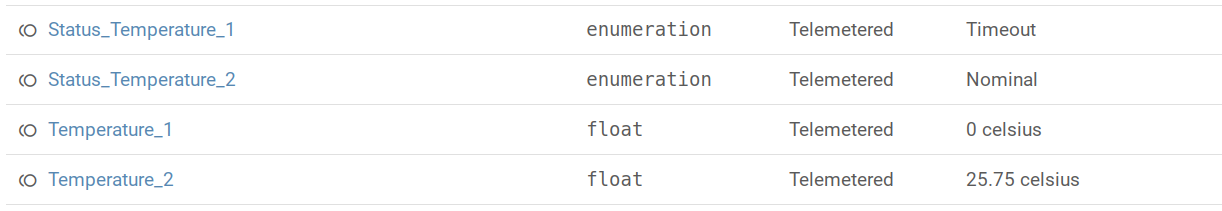
\includegraphics{screenshots/yamcs_f010_parameters}
	\caption{\acs{YAMCS} temperature parameters under the \texttt{F-010} failure}
	\label{fig:yamcsparametersf010}
\end{figure}

In \Cref{fig:yamcsparametersnominal}, the temperature and status values during nominal operation are shown. The values are received normally and the sensors are sending data. The moment the cable is unplugged, the system sets the status value to \texttt{TIMEOUT}\footnote{This process is performed by the peripheral's driver, and not by the implementation of the \acs{ECSS} services.} as it recognizes the connection failure (\Cref{fig:yamcsparametersf010}). Simultaneously, the temperature value becomes \emph{0}, as there is no active measurement.\footnote{In a real system, it would make sense to keep the previous temperature value. In our case, the value was set to 0 to confirm that a failed peripheral returning incorrect values cannot negatively affect the rest of the system.}

\begin{figure}[h]
	\centering
	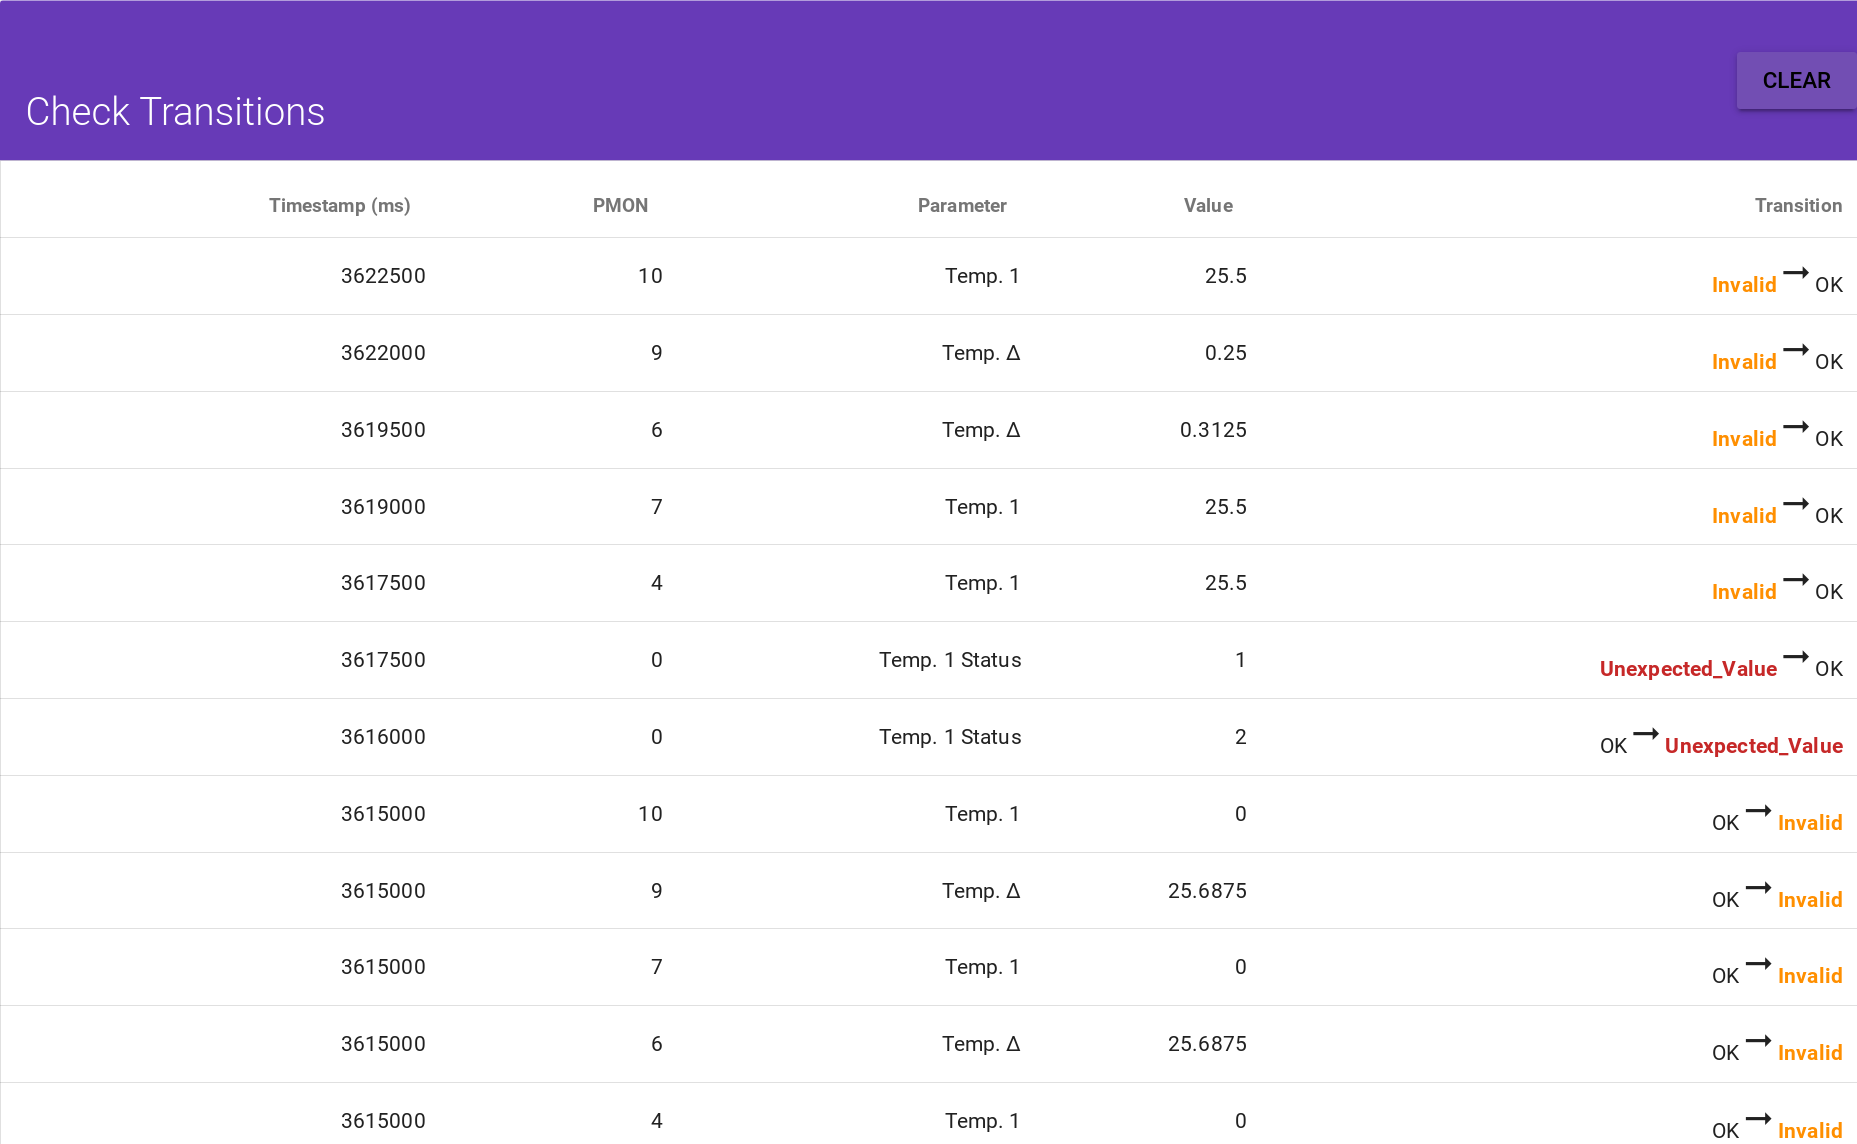
\includegraphics{screenshots/pus_f010_tran}
	\caption{Monitoring definition transitions table (\texttt{F-010} failure as shown in the \acs{PUS} interface)}
	\label{fig:pusf010tran}
\end{figure}

\begin{table*}[h]
	\centering
	\caption[][10pt]{Monitoring definition transitions table (\texttt{F-010} failure)}
	\label{tab:f010tran}
	\begin{tabularx}{\linewidth}{@{}S[table-format=4.0]c@{\hskip 3em}rcl@{\hskip 3em}X@{}}
		\toprule
		\multicolumn{1}{l}{Time (ms)} & \acs{PMON} & \multicolumn{3}{c}{Parameter} & Transition \\ \midrule
		0 & 4 & Temp. 1 & = & 0  & \ok \ar \invalid \\
		0 & 6 & Temp. \(\Delta\) & = & 25.6875 & \ok \ar  \\
		0 & 7 & Temp. 1 & = & 0 & \ok \ar \invalid \invalid \\
		0 & 9 & Temp. \(\Delta\) & = & 25.6875 & \ok \ar \invalid \invalid \\
		0 & 10 & Temp. 1 & = & 0 & \ok \ar \invalid \invalid \\
		1000 & 0 & Temp. Status 1 & = & \texttt{TIMEOUT} & \ok \ar \unexpected \\[1ex]
		\multicolumn{6}{c}{\textcolor{MaterialGrey500}{Failure recovery}} \\[1ex]
		2500 & 0 & Temp. Status 1 & = & \texttt{NOMINAL} & \unexpected \ar \ok \\
		2500 & 4 & Temp. 1 & = & 25.5 & \invalid \ar \ok \\
		4000 & 7 & Temp. 1 & = & 25.5 & \invalid \ar \ok  \\
		4500 & 6 & Temp. \( \Delta \) & = & 0.3125 & \invalid \ar \ok  \\
		7000 & 9 & Temp. \( \Delta \) & = & 0.25 & \invalid \ar \ok  \\
		7000 & 10 & Temp. 1 & = & 25.5 & \invalid \ar \ok  \\ \bottomrule
	\end{tabularx}
\end{table*}

After update the parameter values, the \emph{\texttt{ST[12]} on-board monitoring} service and its monitoring definitions (\Cref{fig:pusf010tran,tab:f010tran}) are next. The following steps are taken in order:
\begin{enumerate}
	\item As soon as the sensor is disconnected, definitions 4, 6, 7, 9, and 10 (\Cref{tab:demo_monitoring}) acquire an \invalid{} state. This happens after deactivation of the \textbf{check validity condition} for these definitions. If sensor 1 is disabled,\footnote{either due to a problem or a command} its values should not be used for any on-board functionality.
	
	Therefore, all definitions associated with sensor 1 are disabled and cannot trigger any reaction. This is done immediately.
	\item After two measurements and time \( 2 \cdot 500 = \SI{1000}{\milli\second} \), monitoring definition 0 confirms that the parameter \emph{Temperature Status 1} has an unexpected value. As a result, the monitoring definition is switched to the \unexpected{} state, therefore triggering the entire fault reporting and recovery process. The sensor failure has now been detected, and the \acs{FDIR} system is now in action.
	\item The monitoring definitions do not change status until the failure is corrected, at which point they return to the \ok{} state. The system has repaired the fault without operator intervention, and has returned to its original state.
\end{enumerate}

\begin{figure}
\centering
\caption[Full list of monitoring definitions during the \texttt{F-010} failure]{Full list of monitoring definitions during the \texttt{F-010} failure, as shown in the \acs{PUS} interface. Definition \emph{0} is enabled while it is pending confirmation of the component's failure, while other sensor-dependent definitions are disabled (\invalid)}.
\label{fig:pusf010moni}
\includegraphics[width=.8\textwidth]{media/screenshots/pus_f010_moni}
\end{figure}

After the failure is detected, the corresponding \textbf{event} is generated and sent to the{operators (\Cref{fig:yamcsf010event}).
		
\begin{figure*}
\centering
\includegraphics{media/screenshots/yamcs_f010_event}
\caption[][-10pt]{The temporary sensor failure event, as shown in \acs{YAMCS}}
\label{fig:yamcsf010event}
\end{figure*}

After the event has been reported, the event-action mechanism is triggered. The action associated with the temporary failure of the sensor is to call the \texttt{restart\_sensor} function.\footnote{\emph{\texttt{ST[08]} function management} service} with an argument value of ``\texttt{1}'', which signals the restart of the 1\textsuperscript{st} sensor. On human observers, the indicator light \textbf{flashes} as the system power-cycles the sensor. This was the first attempt to fix the problem}
	
At this point, as part of the test procedure, the experimenter reconnects the remote sensor, thus simulating the ``fix'' of the problem. The attempts to communicate with the sensor are now successful, and the system assumes that the fault has been repaired.
	
\begin{figure}[h]
		\centering
		\includegraphics{screenshots/yamcs_f010_trend}
		\caption[View of the temperature parameter during a failure]{View of the temperature parameter during a failure. The value is nominal, drops to \SI{0}{\celsius} for 1 second, and is restored after the failure has been corrected.}
		\label{fig:yamcsf010trend}
\end{figure}

\begin{figure}
	\begin{cminted}{text}
3622076 [debug  ] T [T1]: 25.56
3622176 [debug  ] T [T2]: 25.56
3622206 [error  ] Error in TWI: 1
3622206 [debug  ] T [T1]: 0.00
3622307 [debug  ] T [T2]: 25.56
3622336 [error  ] Error in TWI: 1
3622336 [debug  ] T [T1]: 0.00
3622438 [debug  ] T [T2]: 25.63
3622467 [error  ] Error in TWI: 1
3622467 [debug  ] T [T1]: 0.00
3622500 [error  ] Monitoring status 4 changed from 0 to 2
3622500 [error  ] Monitoring status 6 changed from 0 to 2
3622501 [error  ] Monitoring status 7 changed from 0 to 2
3622502 [error  ] Monitoring status 9 changed from 0 to 2
3622502 [error  ] Monitoring status 10 changed from 0 to 2
3622503 [trace  ] New TM [3,25]
Received TM [25]
3622569 [debug  ] T [T2]: 25.63
3622597 [error  ] Error in TWI: 1
3622597 [debug  ] T [T1]: 0.00
3622655 [trace  ] New TM [12,12]
Received TM [82]
3622700 [debug  ] T [T2]: 25.56
3622728 [error  ] Error in TWI: 1
3622728 [debug  ] T [T1]: 0.00
3622831 [debug  ] T [T2]: 25.56
3622859 [error  ] Error in TWI: 1
3622859 [debug  ] T [T1]: 0.00
...
	\end{cminted}
	\caption[Microcontroller diagnostic output during the \texttt{F-010} failure]{Microcontroller diagnostic output during the \texttt{F-010} failure. Once the cable is disconnected, the \acs{MCU} detects the fault on the \acs{I2C} bus, and the read temperature value becomes zero. The state of the monitoring definitions changes on the corresponding clock pulse. Simultaneously, the beacon (\texttt{[3,25]}) and transition reporting \acs{TM} (\texttt{ST[12,12]}) are generated. This diagnostic data is provided in plain-text format by the microcontroller, and will not be available in orbit.}
\end{figure}

\clearpage
\paragraph{\textbf{\texttt{F-020}: Permanent loss of function}}\hspace{0pt}

This failure is similar to \texttt{F-010}, but it presumes that the component cannot be repaired, even after a power-cycle.

\subparagraph{Procedure}
\begin{compactenum}
	\item Disconnect the \acs{SDA} or \acs{SCL} cable from the breadboard
\end{compactenum}

\subparagraph{Visual indications} The 1\textsuperscript{st} \acs{LED} light flashes once, stays on, and then turns off permanently.

\subparagraph{Results}
\begin{table*}[h]
	\centering
	\caption[][10pt]{Monitoring definition transitions table (\texttt{F-020} failure)}
	\label{tab:f020tr}
	\begin{tabularx}{\linewidth}{@{}S[table-format=4.0]c@{\hskip 3em}rcl@{\hskip 3em}X@{}}
		\toprule
		\multicolumn{1}{l}{Time (s)} & \acs{PMON} & \multicolumn{3}{c}{Parameter} & Transition \\ \midrule
		0 & 4 & Temp. 1 & = & 0 & \ok \ar \invalid \\
		0 & 6 & Temp. \(\Delta\) & = & 29.9375 & \ok \ar \invalid \\
		0 & 7 & Temp. 1 & = & 0 & \ok \ar \invalid \\
		0 & 9 & Temp. \(\Delta\) & = & 29.9375 & \ok \ar \invalid \\
		0 & 10 & Temp. 1 & = & 0 & \ok \ar \invalid \\
		1 & 0 & Temp. Status 1 & = & \texttt{TIMEOUT} & \ok \ar \unexpected \\%[1ex]
		2.5 & 2 & Temp. Status 1 & = & \texttt{TIMEOUT} & \ok \ar \unexpected \\[1ex]
		\multicolumn{6}{c}{\textcolor{MaterialGrey500}{Failure isolation}}\\[1ex]
		4 & 0 & Temp. Status 1 & = & \texttt{DISABLED} & \unexpected \ar \ok \\
		5.5 & 2 & Temp. Status 1 & = & \texttt{DISABLED} & \unexpected \ar \ok \\
		\bottomrule
	\end{tabularx}
	\vspace{10pt}
\end{table*}

In this test, the system normally recognizes the sensor failure as expected, and, as shown in \Cref{tab:f020tr}, tries to correct it twice:
\begin{enumerate}
	\item (\( t = \SI{1}{\second}\)) As in the \texttt{F-010} failure, a sensor power-cycle is performed. However, the \emph{Temperature State 1} parameter continues to have an unexpected value after the restart, so the \acs{FDIR} process is not interrupted.
\item (\(t = \SI{2.5}{\second}\)) Monitoring definition \texttt{2} has measured the state of the sensor 5 times (\emph{repetition count}), without any in-bounds values. The system assumes that the fault cannot be corrected, and \textbf{turns off} the sensor completely.

Using this method, the fault is isolated and cannot affect the rest of the system. All \acs{FDIR} definitions associated with the sensor are disabled. The \acl{GS} is aware of the sensor's status via telemetry, and does not take into account its erroneous temperature readings.
\end{enumerate}

At this point, the inactive sensor can only be reset by \acs{TC}, or by rebooting the system. Through the \acs{YAMCS} interface, the user can send the \mintinline{cpp}{/fdirdemo/Set_Temp1_Status(Temperature_Status: "Nominal")} command, thus reactivating the sensor.\footnote[][2ex]{Internally, this command calls the \emph{\texttt{ST[20]} parameter management} service, and sets the \emph{Temperature 1 Status} parameter to \texttt{NOMINAL}}. After recovery, any sensor failure will repeat the same \acs{FDIR} process again.

More generally, we observe that the \acs{FDIR} service does not cause any degradation of the rest of the system, as it is executed as a separate \acs{RTOS} process.

\clearpage
\paragraph{\textbf{\texttt{F-040}: Temporary Value Shift}}\hspace{0pt}

This fault requires the temperature value to be changed for a short period of time. As the temperature must drop below \SI{-40}{\celsius} or rise above \SI{100}{\celsius} to trigger the \acs{FDIR} mechanism (\Cref{tab:hsia}), the only practical method to simulate this failure is to \textbf{insert a false value via software}.

The means we used insert false values is to press\textbf{one of the two buttons} on the development board.\footnote{Alternatively, test telecommands can be used.} More specifically, by pressing \emph{button 0}, the value \SI{80}{\celsius} is added to temperature 1. By pressing \emph{button 1}, the same happens for temperature 2.

\subparagraph{Procedure}
\begin{compactenum}
	\item Hold down \emph{button 0} for 2 seconds only.
\end{compactenum}

\subparagraph{Visual indications} The 1\textsuperscript{st} \acs{LED} light flashes once and stays on.

\subparagraph{Results}
\begin{table*}[h]
	\centering
	\caption{Monitoring definition transitions table (\texttt{F-040} failure)}
	\label{tab:f040tran}
	\begin{tabularx}{\linewidth}{@{}S[table-format=4.0]c@{\hskip 3em}rcl@{\hskip 3em}X@{}}
		\toprule
		\multicolumn{1}{l}{Time (s)} & \acs{PMON} & \multicolumn{3}{c}{Parameter} & Transition \\ \midrule
		0 & 4 & Temp. 1 & = & 109.4375 & \ok \ar \hilim \\[1ex]
		\multicolumn{6}{c}{\textcolor{MaterialGrey500}{Failure recovery}}\\[1ex]
		1.5 & 4 & Temp. 1 & = & 29.5625 & \hilim \ar \ok \\
		\bottomrule
	\end{tabularx}
	\vspace{10pt}
\end{table*}

In this example, only one tracking definition goes out of bounds. As soon as the out-of-bounds is detected, the sensor is restarted, and the fault is corrected.

The logic we used in the \acs{FDIR} architecture means that the remaining definitions continue to monitor the sensor's temperature value, without attaining an \invalid{} value. To avoid any conflict between the definitions, the number of iterations of their measurements should be greater than the one triggered currently. Indeed, in this experiment, no other definition status was changed before and after the failure-related actions.\footnote{Alternatively, utilisation of the \emph{check validity conditions} can ensure that the value does not violate the bounds of another definition.}


\begin{figure*}[h]
	\centering
	\includegraphics[width=\textwidth]{screenshots/yamcs_f040_trend}
	\caption[View of the temperature parameter during the \texttt{F-040} failure]{View of the temperature parameter during the \texttt{F-040} failure, showing the overly large value introduced by the software.}
	\label{fig:yamcsf040trend}
\end{figure*}

\clearpage
\paragraph{\textbf{\texttt{F-050}: Permanent Value Shift}}\hspace{0pt}

This fault is similar to \texttt{F-040}, but with sensor repair being impossible.

The means we used insert false values is to press\textbf{one of the two buttons} on the development board.\footnote{Alternatively, test telecommands can be used.} More specifically, by pressing \emph{button 0}, the value \SI{80}{\celsius} is added to temperature 1. By pressing \emph{button 1}, the same happens for temperature 2.

\subparagraph{Procedure}
\begin{compactenum}
	\item Hold down \emph{button 0} until the 1\textsuperscript{st} \acs{LED} is turned off.
\end{compactenum}

\subparagraph{Visual indications} The 1\textsuperscript{st} \acs{LED} light flashes once, stays on, and then turns off permanently.

\subparagraph{Results}
\begin{table*}[h]
	\centering
	\caption{Monitoring definition transitions table (\texttt{F-050} failure)}
	\label{tab:f050tran}
	\begin{tabularx}{\linewidth}{@{}S[table-format=4.0]c@{\hskip 3em}rcl@{\hskip 3em}X@{}}
		\toprule
		\multicolumn{1}{l}{Time (s)} & \acs{PMON} & \multicolumn{3}{c}{Parameter} & Transition \\ \midrule
		0 & 4 & Temp. 1 & = & 109.4375 & \ok \ar \hilim \\
		1.5 & 7 & Temp. 1 & = & 109.4375 & \ok \ar \hilim \\[1ex]
		\multicolumn{6}{c}{\textcolor{MaterialGrey500}{Failure isolation}}\\[1ex]
		1.5 & 9 & Temp. \( \Delta \) & = & -79.9375 & \ok \ar \invalid \\
		1.5 & 10 & Temp. 1 & = & 109.4375 & \ok \ar \invalid \\
		2 & 4 & Temp. 1 & = & 109.4375 & \hilim \ar \invalid \\
		2 & 6 & Temp. \( \Delta \) & = & -79.9375 & \ok \ar \invalid \\
		2 & 7 & Temp. 1 & = & 109.4375 & \hilim \ar \invalid \\
		\bottomrule
	\end{tabularx}
	\vspace{10pt}
\end{table*}

The \acs{FDIR} process is again two-stepped:
\begin{enumerate}
	\item After the first detection (definition \texttt{4}), the sensor is power-cycled, and the \acs{LED} blinks. The issue is however still not resolved.
	\item After \SI{1.5}{\second}, definition \texttt{7} takes over. Since the value of the sensor is still beyond limits, the action taken is to disable the sensor. This is how the failure is isolated.
	
	After isolation, where the status of the sensor is set to \texttt{DISABLED}, the defitions that depend on the peripheral are also disabled (\invalid). As expected, isolation is now complete.
\end{enumerate}

The isolation \& recovery steps are the same as the ones from failure \texttt{F-020}, and operator intervention is once again required before any other measure is taken.


\clearpage
\paragraph{\textbf{\texttt{F-040} and \texttt{F-050}: Differential measurement}}\hspace{0pt}

The \texttt{F-040} and \texttt{F-050} failures involve an auxiliary detection method: The \emph{large difference between 2 sensor measurement values}. Given the small threshold defined \Cref{tab:hsia} (\(\lvert \Delta \rvert \leq \SI{5}{\celsius}\)), this test is performed in hardware, by heating one of the two sensors.

\subparagraph{Procedure}
\begin{compactenum}
	\item Warm up one of the sensors with a heating element. Make sure to not increase the temperature too much (\(T < \SI{50}{\celsius}\)), and that the other sensor is heated as little as possible.
\end{compactenum}

\subparagraph{Visual indications (temporary failure)} Both \acs{LED} lights simultaneously flash once and stay on.
\subparagraph{Visual indications (permanent failure)} Both \acs{LED} lights simultaneously flash once, stays on, and then turn off permanently.

\subparagraph{Results}
\begin{table*}[h]
	\centering
	\caption{Monitoring definition transitions table (temporary failure \texttt{F-040}, differential)}
	\label{tab:f040dtran}
	\begin{tabularx}{\linewidth}{@{}S[table-format=4.0]c@{\hskip 3em}rcl@{\hskip 3em}X@{}}
		\toprule
		\multicolumn{1}{l}{Time (s)} & \acs{PMON} & \multicolumn{3}{c}{Parameter} & Transition \\ \midrule
		0 & 6 & Temp. \( \Delta \) & = & -6.1875 & \ok \ar \lolim \\[1ex]
		\multicolumn{6}{c}{\textcolor{MaterialGrey500}{Failure recovery}}\\[1ex]
		7.5 & 6 & Temp. \( \Delta \) & = & -4.8125 & \lolim \ar \ok \\
		\bottomrule
	\end{tabularx}
	\vspace{10pt}
\end{table*}

The differential case recovery actions are similar to the single case (\texttt{F-040}, \texttt{F-050}), with the distinction that is not known to the \acs{MCU} which of the 2 sensors has failed. The architecture here follows a \emph{fail-safe} approach, and disables both sensors. As a consequence, all 7 monitoring definitions that depend on temperature values are disabled (\invalid).

\begin{table*}[h]
	\centering
	\caption{Monitoring definition transitions table (permanent failure \texttt{F-050}, differential)}
	\label{tab:f050dtran}
	\begin{tabularx}{\linewidth}{@{}S[table-format=4.0]c@{\hskip 3em}rcl@{\hskip 3em}X@{}}
		\toprule
		\multicolumn{1}{l}{Time (s)} & \acs{PMON} & \multicolumn{3}{c}{Parameter} & Transition \\ \midrule
		0 & 6 & Temp. \( \Delta \) & = & -5.8125 & \ok \ar \lolim \\
		2.5 & 9 & Temp. \( \Delta \) & = & -6 & \ok \ar \lolim \\[1ex]
		\multicolumn{6}{c}{\textcolor{MaterialGrey500}{Failure isolation}}\\[1ex]
		2.5 & 10 & Temp. 1 & = & 38.3125 & \ok \ar \invalid \\
		2.5 & 11 & Temp. 2 & = & 32.3125 & \ok \ar \invalid \\
		3 & 4 & Temp. 1 & = & 38.3125 & \ok \ar \invalid \\
		3 & 5 & Temp. 2 & = & -32.3125 & \ok \ar \invalid \\
		3 & 6 & Temp. \( \Delta \) & = & -6 & \ok \ar \invalid \\
		3 & 7 & Temp. 1 & = &38.3125 & \ok \ar \invalid \\
		3 & 8 & Temp. 2 & = & 32.3125 & \ok \ar \invalid \\
		3 & 9 & Temp. \( \Delta \) & = & -6 & \ok \ar \invalid \\
		\bottomrule
	\end{tabularx}
	\vspace{10pt}
\end{table*}

\FloatBarrier
\paragraph{\textbf{\texttt{F-060}: \acs{I2C} bus pin output stuck}}\hspace{0pt}

This failure is simulated by connecting an extra cable. Generally, in cases of cable harness modifications, care must be taken so that connections that can harm the test system (e.g.\ short circuits) are avoided, especially if there are no suitable protection circuits.

\subparagraph{Procedure}
\begin{compactenum}
	\item Connect one of the \acs{SDA}, \acs{SCL} pins to ground using an extra jumper wire.\footnote{As the \acs{I2C} bus follows an open drain logic, connecting one of the prots to ground will not cause any further issues to the electronics.}
\end{compactenum}

\subparagraph{Results}
We observe that the results are identical to the ones of the \texttt{F-020} failure (permanent loss of function). This is expected, as we have essentially damaged the \acs{I2C} bus.

\paragraph{\textbf{\texttt{F-070} to \texttt{F-120}: Sensor 2}}\hspace{0pt}

The above tests were repeated for the 2\textsuperscript{nd} sensor. The test results are identical to the ones of the 1\textsuperscript{st} sensor, as the components follow the same specifications and \acs{FDIR} design.

At this point we note that even when the design and the software are identical, it is still necessary to repeat the testing procedures in cases such as this one, as the possibility of hardware errors, wrong connections, misconfigurations and bugs is not eradicated.

\clearpage
\paragraph{\textbf{\texttt{F-130}: Overheating}}\hspace{0pt}

In this test we do not investigate the failure of one of the sensors, but the failure of the subsystem itself, which is assumed to have overheated. To ease execution of this test, we used a virtual temperature increase via software.

\subparagraph{Procedure}
\begin{compactenum}
	\item Call the \texttt{bogus\_temp} \acs{ECSS} function via \acs{TC}. This function causes a gradual increase of the temperature by \SI{90}{\celsius} at maximum.
\end{compactenum}
\marginnote{
Alternatively, a hot air gun or another heat source can be used so that both sensors are heated to \SI{50}{\celsius}. In this case, we need to pay attention to have a uniform temperature increase, so as to not trigger the differential check.
}

\subparagraph{Visual indications} The \acs{MCU} status \acs{LED} stops blinking for a while, and then continues blinking normally. The sensor \acsp{LED} blink once.

\subparagraph{Results}
\begin{table*}[h]
	\centering
	\caption{Monitoring definition transitions table (\texttt{F-130} failure)}
	\label{tab:f130tran}
	\begin{tabularx}{\linewidth}{@{}S[table-format=4.0]c@{\hskip 3em}rcl@{\hskip 3em}X@{}}
		\toprule
		\multicolumn{1}{l}{Time (s)} & \acs{PMON} & \multicolumn{3}{c}{Parameter} & Transition \\ \midrule
		0 & 10 & Temp. 1 & = & 92.288 & \ok \ar \hilim \\
		\multicolumn{6}{l}{\cellcolor{MaterialYellow300}\textcolor{black}{Autonomous \acs{MCU} restart}}\\
		\bottomrule
	\end{tabularx}
	\vspace{10pt}
\end{table*}

In this example, only the monitoring definition connected with the \SI{50}{\celsius} is activated. Once the system spends some time in this temperature, an \acs{MCU} restart takes place immediately. This restart would continue to occur repeatedly, if the temperature remained out of bounds.

This failure essentially belongs to subsystem level, and not unit (sensor) level. We also note that due to the large amount of time between restarts, operators have enough time to receive \acsp{TM} and transmit the necessary \acsp{TC} to deal with the issue.

\begin{figure*}
	\includegraphics{screenshots/yamcs_f130_parameters}
	\caption[Temperature measurements with bogus values added, as seen in YAMCS]{Temperature measurements with bogus values added, as seen in \acs{YAMCS}. The temperature reaches \SI{90}{\celsius}, until the \acs{MCU} restarts, at which point the temperature is restored to nominal levels.}
\end{figure*}

\clearpage
\subsection{Real-time modification of \ac{FDIR}}

The power of \acs{SAVOIR}'s \ac{FDIR} approach lies in the fact that the entire \ac{FDIR} concept can be safely modified via \ac{TC} without requiring any modifications or reuploads of the spacecraft's software. The application of the \acs{ECSS} services paradigm allows customising all on-board \ac{FDIR} functions and associated services using predefined \ac{TC} structures. In this section, \acs{ECSS} commands will be executed to demonstrate these capabilities and their control from the Ground Station.

The level of reconfigurability possible is defined by requirements listed in \parencite{ECSS-E-ST-70-11C,SAVOIR-HB-003}. The tailored version used for our experiments is listed in \Cref{tab:fdir-recon-rq}.

\begin{table*}[h]
	\centering
	\caption{\ac{FDIR} reconfigurability requirements}
	\label{tab:fdir-recon-rq}
	\begin{tabularx}{\textwidth}{@{}lXlL{4cm}@{}}
		\toprule
 		\# & Requirement & Service & Details \\ \midrule
		\texttt{RC-010} & The reporting of FDIR activities shall contain all information for failure analysis (e.g.\ time of occurrence, parameter out‐of‐limit, switching performed). & ST[12] on-board monitoring & Via periodic \emph{check transition reports} \\
		\texttt{RC-020} & The capability shall be provided to enable and to disable any on‐board FDIR function by telecommand. & ST[12] on-board monitoring & Via \emph{enable}/\emph{disable} \emph{parameter monitoring definitions} commands  \\
		\texttt{RC-030} & The capability shall be provided to add and delete parameters from the on‐board monitoring list. & ST[12] on-board monitoring & Via \emph{add}/\emph{delete} \emph{parameter monitoring definitions} commands  \\
		\texttt{RC-040} & The capability shall be provided to modify the failure recovery actions associated with each on-board monitoring definition. & ST[19] event-action & Via \emph{add}, \emph{delete}, \emph{enable} and \emph{disable} \emph{event-action definitions} commands \\ \bottomrule
	\end{tabularx}
\end{table*}

The \ac{YAMCS} platform was once again used to generate the wanted commands (\Cref{fig:yamcs_commands}). This section will analyse how \acs{ECSS} \acsp{TC} can be used to perform the required modifications.

\begin{figure}[h]
	\includegraphics{screenshots/yamcs_commands.png}
	\caption{List of commands in the \acs{YAMCS} interface. These commands can initiate spacecraft actions, enable/disable sensors, or reconfigure the on-board \acs{ECSS} services databases. The list of commands is provided programmatically in \ac{XTCE} format.}
	\label{fig:yamcs_commands}
\end{figure}


\paragraph{\textbf{\texttt{RC-010} \acs{FDIR} observability}}
The degree of observability required, in real and non-real time, is achieved using the interface presented in \Cref{sec:pusinterface}. The ready-made telemetry structures implemented by the \acs{PUS} standard are \autocite{ECSS-E-ST-70-41C}:
\begin{compactitem}
	\item \texttt{TM[3,25]}: Periodic parameter value reporting (beacon)
	\item \texttt{TM[5,1]} to \texttt{TM[5,4]}: Event reports at the time of occurrence
	\item \texttt{TM[12,9]}: List of tracking definitions
	\item \texttt{TM[12,12]}: Periodic reporting of state transitions in monitoring definitions\footnote{In simpler terms, we are informed when a parameter goes out of bounds, and when it returns to nominal state}
	\item \texttt{TM[19,7]} and \texttt{TM[19,11]}: List of event-action definitions
	\item \texttt{TM[20,2]}: Reporting of the value of any parameter in the system
\end{compactitem}

With the above set of telemetry, downlinked either periodically or after \acs{TC}, operators are able to examine the state of the system and its \acs{FDIR} in detail. All results in \Cref{sec:simul} were extracted using the above telemetry structures.

\paragraph{\textbf{\texttt{RC-020} Enabling/Disabling \acs{FDIR}}}


The features implemented and tested that allow controlling \acs{FDIR} functions are as follows:
\begin{itemize}
	\item \texttt{TC[12,16]}: \emph{disable the parameter monitoring function}
	
	This telecommand is defined in the \acs{PUS} standard and allows to completely disable the parameter monitoring function, and by extension, \textbf{completely disable the \acs{FDIR}}. After it is sent, any failure in the system is not detected, and no recovery operations are performed.
	
	It can be understood that such a command is fairly dangerous for the satellite system, as an incorrect execution will greatly reduce the possibility of recovery from a failure.\footnote{Critical commands such as this one are suggested to typically require two sub-commands to be sent in series (ARM--EXECUTE logic)} Nevertheless, it is useful if the \acs{FDIR} experiences problems such as spurious triggers that pose a higher risk to the mission.
	
	We note here that this command does not prevent status queries or configuration changes in the on-board monitoring service.
	
	\item \texttt{TC[12,15]}: \emph{enable the parameter monitoring function}
	
	All \acsp{TC} to disable a function are followed by their ``enable'' counterpart. For example, this telecommand enables the parameter monitoring to be re-enabled if it was previously disabled.

	\item \texttt{TC[12,2]}: \emph{disable parameter monitoring definitions}
	
	In addition to disabling the entire \acs{FDIR} function, the standard allows the possibility to disable only specific pieces of it (in singles or in bulk).
	
	\begin{figure}[h]
		\includegraphics{screenshots/yamcs_send_disablepmon.png}
		\caption[View the \acs{YAMCS} command execution screen]{View the \acs{YAMCS} command execution screen. The user is prompted to enter the single argument to the \texttt{TC[12,1]} command, which is the monitoring definition that they wish to disable.}
		\label{fig:yamcssenddisablepmon}
	\end{figure}
	
	This feature is particularly useful when it appears that \acs{FDIR} is too strict for a component.
	
	\item \texttt{TC[12,1]}: \emph{enable parameter monitoring definitions}
	
	\item \texttt{TC[19,5]}: \emph{disable event-action definitions}
	
	In addition to disabling the entire \acs{FDIR} for a component, it is possible to disable only the ``IR''\footnote{\textcolor{MaterialGrey400}{Detection, }Isolation \& Recovery} part of it. This means that while failures are detected, no attempt is made to isolate or repair them. In this way, we can disable the \acs{FDIR}, but maintain observability of parameters and bound violations.

	In technical terms, this command disables the event-action definitions for specific events. The behaviour of a typical failure after executing this command is shown in \Cref{tab:eaofftr}.

\begin{table*}[h]
	\centering
	\caption[Transition table with event-actions disabled]{Transition table with event-actions disabled. The sensors are not disabled by the \acs{FDIR}, but the event-action definitions go out of bounds one-by-one.}
	\label{tab:eaofftr}
	\begin{tabularx}{\linewidth}{@{}S[table-format=4.0]c@{\hskip 3em}rcl@{\hskip 3em}X@{}}
		\toprule
		\multicolumn{1}{l}{Time (s)} & \acs{PMON} & \multicolumn{3}{c}{Parameter} & Transition \\ \midrule
		0 & 4 & Temp. \(\Delta\) & = & 110.625 & \ok \ar \hilim \\
		1.5 & 7 & Temp. \( \Delta \) & = & 110.6875 & \ok \ar \hilim \\
		2 & 6 & Temp. \( \Delta \) & = & -79.9375 & \ok \ar \lolim \\
		4.5 & 9 & Temp. \( \Delta \) & = & -79.875 & \ok \ar \lolim \\
		5 & 10 & Temp. \( \Delta \) & = & 110.625 & \ok \ar \hilim \\
		\bottomrule
	\end{tabularx}
	\vspace{10pt}
\end{table*}

\item \texttt{TC[19,4]}: \emph{enable event-action definitions}
	
\end{itemize}

\paragraph{\textbf{\texttt{RC-030} Addition/Deletion of monitoring definitions}}\hspace{0pt}
	
	The ability to delete and add new \acs{FDIR} definitions is provided via the \emph{\texttt{ST[12]} on-board monitoring} service \acsp{TC}:
	
	\begin{itemize}
	\item \texttt{TC[12,5]}: \emph{add parameter monitoring definitions}
	
	Through \texttt{TC[12,5]} we can provide the satellite with all the data needed to create a monitoring definition, for any type of parameter, value check and check validity condition.
	
	\begin{figure}[h]
		\includegraphics{tc125}
		\caption{The \texttt{TC[12,5]} telecommand, exactly as shown in \autocite{ECSS-E-ST-70-41C}}
	\end{figure}
	
	The arguments to this command can be given from within the \acs{YAMCS} interface (\Cref{fig:yamcs_add_definition}).
	
	\begin{figure}[h]
		\centering
		\includegraphics[width=\textwidth]{screenshots/yamcs_add_definition}
		\caption{Add tracking definition environment from \acs{YAMCS}}
		\label{fig:yamcs_add_definition}
	\end{figure}
	
	Note that using this command presents some difficulties, due to the many different possible types of parameters and controls, leading to different message formats. For this reason, in this example we only implemented the \mintinline{cpp}{uint64_t} type for expected value checks, and \mintinline{cpp}{float} for limit checks. Definitions with the previous datatypes were coded so as to be compatible with all other numerical parameters in the space segment code.
		
	\item \texttt{TC[12,6]}: \emph{delete parameter monitoring definitions}
		
		This command can delete monitoring definitions, and, when used with \texttt{TC[12,5]}, can modify monitoring definitions.
		
		Note that modification via \emph{delete-and-add} is not recommended by \acs{SAVOIR} \autocite{SAVOIR-HB-003}, as it runs the risk that one of the two commands will not be executed, and the system will be in an undesirable state. \emph{\texttt{TC[12,7]} modify parameter monitoring definitions} can be used to remedy this issue, which was however not implemented for this demonstration.
		
	\end{itemize}
	
	\paragraph{\textbf{\texttt{RC-040} Addition/Deletion of event-action definitions}}\hspace{0pt}
	
	Similar to the aforementioned \acsp{TC}, operators can modify the list of event-action definitions, or even link them to specific monitoring definitions, by taking advantage of the \emph{\texttt{ST[19]} eventaction} service functions. In all of the following functions, the definitions are accessed based on the Application Process ID and the event ID.
	

		
	\begin{itemize}
		\item \texttt{TC[19,1]}: \emph{add event-action definitions}
		
		Note that the \emph{action} part is defined by the user as a \textbf{nested \acs{TC} packet}. Thus, by providing arbitrary telecommand, operators can instruct the satellite to perform virtually any action after a failure.
		
		\item \texttt{TC[19,2]}: \emph{delete event-action definitions}
		
	\end{itemize}

\chapter{Conclusion and Future Work}
\label{cap:conclusion}

\begin{fullwidth}
This thesis presented the architecture and implementation of a method to detect, isolate and recover from failures in low-cost space systems. In \Cref{cap:acubesat}, the AcubeSAT mission was presented, along with details related to its reliability. In \Cref{cap:savoir}, the \texttt{ECSS-E-ST-70-41C} and \texttt{SAVOIR-HB-003} standards were presented, showing their proposed methods for a structured programmatic framework and a modular fault correction architecture. The 7 steps of the \acs{FDIR} implementation were also presented, starting with requirements definition, continuing with design, and ending with implementation and verification. Furthermore, the concept of \acf{FMEA} and its coupling with software was presented. In \Cref{cap:acufdir}, the previous information was made more concrete through its application to the design of the AcubeSAT nanosatellite. More specifically, the \acs{FDIR} principles were set, and a theoretical analysis of different architectures was performed. Finally, the pool of all possible fault detection, prevention and recovery actions available on the nanosatellite was presented, along with flowcharts showing the specific procedures in every system mode.

In \Cref{cap:practical}, the 7 steps of the \acs{FDIR} process were applied to a mock satellite system. The hardware setup made of an \acs{MCU} and two temperature sensors was supplemented with implementations of the aforementioned standards, as well as a \acl{GS} simulation platform. The design of the \acs{FDIR} for this application was based on a complete \acs{FMEA} of the system, based on which the monitored parameters, value thresholds and corrective actions were extracted. This procedure was carried out for all possible failures of the system. Each of those failures was then simulated in hardware or in software, and it was shown that the system could recover in each case. Finally, the ability to parameterise the \acs{FDIR} in orbit without software modifications was demonstrated.

The result of the above study and tests shows that it is possible to apply the \acs{SAVOIR} method to repair faults on a nanosatellite. The proposed logic can be supported by a low-resource microcontroller, and the developed software can be used ``as-is'' for any vulnerable system, which is possible thanks to the scalable proposed architecture. The use of such a structured approach is believed to greatly increase the survival chances of a CubeSat in orbit, but also to reduce the development time of a mission, as proven standards and available software can be used. All the libraries that were employed are open source and available for use, but could also be freely replaced with counterparts offering the same functionality.

The importance of \textbf{verification} and \textbf{tests} of the developed implementation must be further stressed. The closer the test conditions are to the actual in-orbit conditions, the higher the confidence in the implemented mechanisms. In our own tests we found a significant number of deficiencies, edge cases and race conditions that were not obvious during the design and naive tests, but appeared directly in the tests of each individual failure.

Despite the potential offered by such a system, we noted the following implementation details that require attention:
\begin{itemize}
	\item A hasty implementation of \acs{FDIR} can lead to a large increase in complexity, and difficulty managing all reliability definitions. Complexity increases the possibility of human error, undetected errors, and system malfunction. In non-critical systems, it is suggested that the number of definitions be limited to a manageable number, preventing over-design. In our example, monitoring of the \(\Delta\) difference of temperatures could be skipped, in favour of triggering a system restart only when both sensors are out of range.
	\item The different types of parameter variables (\mintinline{cpp}{uint16_t}, \mintinline{cpp}{uint32_t}, \mintinline{cpp}{float} etc.) pose technical challenges in type-safe environments (such as that of C++), and it may be necessary to use more ``unsafe'' structures and pointers, rather than a templated implementation.
	\item It is important to consider the correlations between monitoring definitions, and to ensure that one definition does not cause another to trigger faster or slower (e.g.\ due to a sensor restart that resets all other definitions).
	\item The \texttt{ECSS-E-ST-70-41C} standard does not provide flexibility in defining ``smart'' parameters, and data such as the \emph{difference between values} must be manually defined in the code. In addition, there is reduced flexibility in defining multiple event-action definitions, as each event can be associated with only one configurable reaction.
\end{itemize}

\section{Future work}

This thesis presented only a case study and an experimental setup to verify a subset of the \acs{FDIR} functionality. This next steps of the process still need to be applied during the development of AcubeSAT's engineering and flight models, during assembly and integration of the AcubeSAT nanosatellite, and during the subsystem-level and system-level verification campaigns. Finally, in-orbit results about the performance of the \acs{FDIR} can be extracted after the possible AcubeSAT launch.

In addition to the continued implementation of \acs{FDIR} on the nanosatellite, some more specific objectives are:
\begin{itemize}
	\item Continuation of the implementation of the \acs{ECSS} services. Code development implementing:
	\begin{compactitem}
		\item Modification of monitoring definitions
		\item Monitoring of multiple variables with \texttt{OR} or \texttt{AND} conditions (``functional monitoring definitions'')
		\item Support of arbitrary data types for parameters
		\item Preparation of unit tests for software-level verification
	\end{compactitem}
	\item Completion of the Mission Control software for the central \acl{GS}, and integration with the \acs{ECSS} service database 
	\item Extension of the detailed \acs{FDIR} design to Safe Mode
	\item Comparison with other satellite control architectures and \acs{FDIR} philosophies typically used in the industry \parencite{NASA-HDBK-1002,zolghadri_advanced_modelbased_2012}
	\item Extension of the theoretical analyses (\Cref{sec:theoretical}) and incorporation of parameters such as cost \parencite{chang_development_reliabilitycorrected_2013}, complexity, past experience and further architectures
	\item Study of modern reliability assessment techniques and their application to the nanosatellite, during design or in orbit
	\item Planning of tests to extract actual component reliability results (e.g.\ heavy ion radiation tests)
\end{itemize}




\end{fullwidth}

%\backmatter
\appendix

\begin{fullwidth}
\printbibliography[heading=bibnumbered]
\end{fullwidth}


\printindex



\end{document}

